\documentclass{scrreprt}
\usepackage[ngerman]{babel}
\usepackage[utf8]{inputenc}
\setlength{\parskip}{5.5pt}
\setlength{\parindent}{1em}
\usepackage{hyperref}
\usepackage{amssymb,amsmath,amsthm,enumitem}
\usepackage{mathtools}
\usepackage{algpseudocode}
\usepackage{algorithm}
\usepackage{natbib}
\usepackage{graphicx}
\usepackage[normalem]{ulem}
\usepackage{soul}
\usepackage{color}
\usepackage[table,xcdraw]{xcolor}
\usepackage{fancyhdr}
\usepackage{amsfonts}
\usepackage{booktabs}
\usepackage{siunitx}
\usepackage{longtable}
\usepackage{enumitem}
\usepackage{pdflscape}
\usepackage{listings} 
\usepackage[toc,page]{appendix}
\usepackage{geometry}
\usepackage[T1]{fontenc}% wichtig für Trennung von Wörtern mit Umlauten
\usepackage{microtype}% verbesserter Randausgleich

\DeclareMathOperator*{\argmax}{arg\,max}
\DeclareMathOperator*{\maxi}{max}
\DeclareMathOperator*{\mini}{min}
\DeclareMathOperator*{\counti}{count}
\DeclareMathOperator*{\meani}{mean}
\DeclareMathOperator*{\mediani}{median}
\DeclareMathOperator{\ReX}{ReX}
\DeclareMathOperator{\ImX}{ImX}



% design

\geometry{a4paper,left=30mm,right=30mm, top=30mm, bottom=35mm minus 5mm} 
\usepackage[skip=5pt]{caption}
\setlength{\footskip}{15mm}

\pagestyle{fancy}
\fancyhf{}
\chead{\nouppercase{\rightmark}}
\cfoot{\thepage}

\widowpenalty10000
%\clubpenalty10000



\title{Visualisierung kontinuierlicher, multimodaler Schmerz Scores am Beispiel akustischer Signale}
\subtitle{Masterarbeit}
\author{Franz Anders \\ HTWK Leipzig }
\date{Januar 2017}



\begin{document}
	
%\setlength{\abovedisplayskip}{0pt plus 2pt minus 2pt}
%\setlength{\belowdisplayskip}{10pt plus 2pt minus 2pt}
%\setlength{\abovedisplayshortskip}{-5pt plus 2pt minus 2pt}
%\setlength{\belowdisplayshortskip}{10pt plus 2pt minus 2pt} 

%\setlength{\intextsep}{10mm plus 1mm minus 5mm}

\maketitle

\pagenumbering{Roman} 

\chapter*{Abstract}

\tableofcontents
\listoffigures


\chapter{Einleitung}

\pagenumbering{arabic} 

\chapter{Grundlagen der Schmerzbewertung mit Hilfe akustischer Signale}
\label{sec:foundations}

%Nochemal lesen!
Das Ziel dieses Kapitels ist es, wichtige Grundlagen zu erläutern, die zum Verständnis des in dieser Arbeit vorgestellten Konzeptes und den dabei angewandten Methoden notwendig sind. Dazu werden in \autoref{sec:signal_foundations} zunächst einige Teilaspekte der Audiosignalverarbeitung besprochen, welche insbesondere bei der akustischen Modellierung der menschlichen Stimme Anwendung finden. In \autoref{sec:medicalFoundations} werden Methoden zur Schmerzbewertung bei Neugeborenen beschrieben. Die Schmerzdiagnostik wird zunächst aus Sicht medizinischer Fachkräfte im klinischen Alltag beleuchtet. Weiterhin wird eine Einführung in die \glqq Schreiforschung\grqq{} gegeben, einem Wissenschaftsgebiet, bei dem das Weinen von Neugeborenen mit Methoden der Signalverarbeitung tiefergehend analysiert wird. In \autoref{sec:learning} werden Grundlagen des überwachten maschinellen Lernens erläutert, da diese im Zusammenhang mit der Erkennung von Schreigeräuschen in Audiosignalen sowie der automatisierten Schmerzbewertung Einsatz finden.

\section{Grundlagen der Verarbeitung akustischer Signale}
\label{sec:signal_foundations}

Der erste Schritt zur Schmerzdiagnostik auf Basis akustischer Informationen des Weinens von Neugeborenen ist, dieses Weinen mit einem Mikrofon aufzunehmen und in ein digitales Signal zu wandeln. In diesem Abschnitt werden Grundlagen zur Verarbeitung eines solchen digitalen Signals erläutert. Es wird ein grundlegendes Verständnis dieses Bereichs vorausgesetzt. Falls dieses Verständnis nicht vorhanden ist, wird zur Einarbeitung das Buch \glqq The Scientist and Engineer's Guide to Digital Signal Processing\grqq{} von Steven W. Smith empfohlen \cite{dspGuide}, welches vom Autor kostenlos als E-Book bereitgestellt wird.

\subsection{Grundlegende Definitionen}

Ein digitales Signal $x[\;]$ ist eine beliebige Zahlenfolge mit diskretem Definitionsbereich. Dem Definitionsbereich kommt die Bedeutung \emph{Zeit} zu.\cite[S. 11-12]{dspGuide} In dieser Arbeit gilt die Konvention, dass mit $x[\;]$ das \emph{gesamte} Signal und mit $x[n]$ \emph{ein} Wert des Signals zum \emph{Zeitpunkt} oder \emph{Index} $n$ gemeint ist. Ein Wert $x[n]$ wird auch als \emph{Sample} bezeichnet. Die Samplingfrequenz des digitalen Signals wird mit $f_s$ bezeichnet.

Der Indexbereich eines Signals erstreckt sich implizit immer von negativer bis positiver Unendlichkeit. Das heißt nicht, dass alle Samples des Signals auch Informationen enthalten müssen. Der \emph{Support} ist das kleinst mögliche Zeitintervall, außerhalb dessen alle Samples des Signals den Wert 0 haben, wie \autoref{eq:support} definiert. Ein Sample mit dem Wert 0 wird in dieser Arbeit auch als \glqq 0-Sample\grqq{} bezeichnet.\cite[S. 24]{dspMichigan}

\begin{equation}
\label{eq:support}
\begin{split}
\text{Sup}(x[\;]) = [sup_s, sup_e] \quad , sup_s, sup_e \in \mathbb{Z} \\  \forall n \not\in [sup_s, sup_e] : x[n] = 0
\end{split}
\end{equation}

Die \emph{Dauer} eines Signals entspricht der Länge des Supportes nach \autoref{eq:duration}. In dieser Arbeit gilt die Konvention, dass die Länge eines Signals mit der Variable $N$ abgekürzt wird. Wenn nicht explizit anders definiert, erstreckt sich der Support eines Signals über das Intervall $0 ,\ldots, N-1$.\cite[S. 24]{dspMichigan}

\begin{equation}
\text{Length}(x[\;]) = sup_e - sup_s + 1 = N
\label{eq:duration}
\end{equation}


\subsection{Statistische Merkmale von Signalen}

Im folgenden wird ein Überblick über wichtige statistische Merkmale von Signalen gegeben.

\begin{enumerate}[leftmargin=*]
	
	\item Der \textbf{Maximalwert/Minimalwert} beschreibt den höchsten/niedrigsten in  $x[\;]$ enthaltenen Wert nach \autoref{eq:maxAndMin}.
	
	\begin{equation}
	\begin{gathered}
	\max(x[\;]) = \max\limits_{n \in \text{Sup}(x[\;]) }\{\ x[n]\ \} \\ 
	\min(x[\;])= \min\limits_{n \in \text{Sup}(x[\;])}\{\ x[n]\ \}
	\end{gathered}
	\label{eq:maxAndMin}
	\end{equation}
	
	
	\item Der \textbf{Durchschnittswert} (engl. \emph{Average Value}) beschreibt den durchschnittlichen Wert aller Samples von $x[\;]$ nach \autoref{eq:avg}.
	
	\begin{equation}
	\text{AVG}(x[\;]) = \frac{1}{N} \sum_{n = 0}^{N-1} x[n]
	\label{eq:avg}
	\end{equation}
	
	\item Der \textbf{Mean Squared Value} (\emph{MSV}) beschreibt den Durchschnittswert aller quadrierten Samples nach \autoref{eq:msv}. Er wird im Deutschen auch als \emph{durchschnittliche Energie} oder \emph{quadratisches Mittel} bezeichnet.
	
	\begin{equation}
	\text{MSV}(x[\;]) = \frac{1}{N} \sum_{n = 0}^{N-1} x[n]^2
	\label{eq:msv}
	\end{equation}
	
	\item Der \textbf{Root Mean Square} (\emph{RMS}) wird definiert als die Wurzel des Mean Squared Value nach \autoref{eq:rms}. Der RMS kann im Vergleich zum MSV intuitiver ins Verhältnis zu den Werten des Signals gesetzt werden kann. Er wird im Deutschen auch als \emph{Wurzel des quadratischen Mittels} bezeichnet.
	
	\begin{equation}
	\text{RMS}(x[\;]) = \sqrt{\frac{1}{N} \sum_{n = 0}^{N-1} x[n]^2}
	\label{eq:rms}
	\end{equation}
	
	\item Die \textbf{Energie} (engl. \emph{Energy}) eines Signals wird nach \autoref{eq:energy} definiert. Sie entspricht dem MSV-Wert multipliziert mit der Länge des Intervalls.\cite[S. 27-28]{dspMichigan}
	
	\begin{equation}
	\text{E}(x[\;]) = \sum_{n = 0}^{N-1} x[n]^2
	\label{eq:energy}
	\end{equation}
	
\end{enumerate}	

%\begin{figure}[h]
%	\centering
%	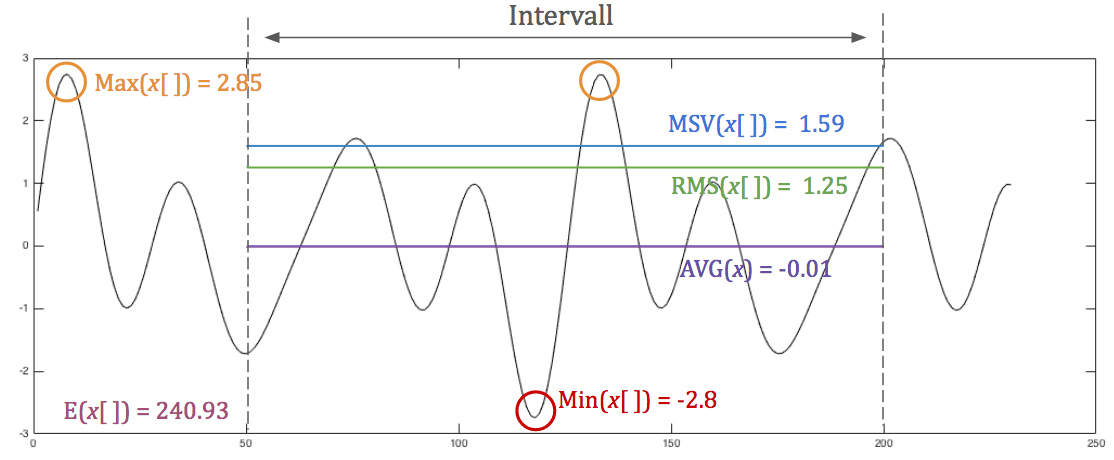
\includegraphics[width=0.9\textwidth]{bilder/sigStats02.png}
%	\caption{Statistische Merkmale eines Beispielsignals über dem Intervall [50,200]}
%	\label{img:sigStats}
%\end{figure}

\subsection{Fehlersignale}

Angenommen, ein Signal $x[\;]$ wird übertragen, auf dem Übertragungsweg jedoch durch ein anderes Störsignal, wie z.B. Rauschen, $e[\;]$ überlagert. $e[\;]$ wird in diesem Zusammenhang als das \emph{Fehlersignal} bezeichnet. Dann wird das resultierende \emph{Nutzsignal} $x'[\;]$ nach \autoref{eq:sigErrorAddition} durch Addition des Signals und des Fehlersignals berechnet.\cite[S. 29]{dspMichigan}

\begin{equation}
x'[n] = x[n] + e[n]
\label{eq:sigErrorAddition}
\end{equation}

Eine Möglichkeit der Quantifizierung der Stärke des Rauschens im Vergleich zum Signal ist, den MSV des Eingangssignal ins Verhältnis zum MSV des Fehlersignals zu setzen. In der Praxis ist der MSV des Eingangssignals meist sehr viel höher als der des Fehlersignals. Um den Zahlenraum zu begrenzen, wird die Pseudoeinheit dB verwendet. \autoref{eq:snrDb} definiert den \emph{Signal-Rausch-Abstand} (\emph{SNR}, englisch Signal-to-Noise-Ratio). Ein \emph{niedriger} SNR weist auf ein \emph{starkes} Rauschen hin und ein \emph{hoher} SNR auf ein \emph{schwaches} Rauschen. Im Zusammenhang mit der Spracherkennung ist der Signal-Rausch-Abstand von Bedeutung, da ein höheres Rauschen die Verarbeitung des Nutzsignals, der Sprache, erschwert.\cite{matlabSNR}

\begin{equation}
\text{SNR}(x[\;],e[\;]) = 10 \cdot  \log \Big(\frac{MSV(x[\;])}{MSV(e[\;])} \Big) \text{ dB}
\label{eq:snrDb}
\end{equation}

\subsection{Kurzzeit-Fourier-Transformation}
\label{sec:stft}

Das Signal $x[\;]$ befindet sich im \emph{Zeitbereich}, da die unabhängige Variable die Zeit beschreibt. \autoref{eq:complexDFTpolar} definiert die \emph{komplexe diskrete Fouriertransformation}, kurz \emph{DFT}. Wird diese Transformation für $k = 0 , \ldots , N-1$ durchgeführt, wird das diskrete Signal $x[\;]$ aus dem Zeitbereich in den Frequenzbereich $X[\;]$ überführt. Hat ein Signal im Zeitbereich die Länge $N$, so hat der entsprechende Frequenzbereich die selbe Länge. Jedes Sample des Frequenzbereiches ist eine komplexe Zahl, deren Realteil $\Re(X[k])$ die Amplitude der entsprechenden Sinuswelle mit der Frequenz $f = k\frac{f_s}{N}$ bezeichnet und deren Imaginärteil  $\Im(X[k])$ die Amplitude der entsprechenden Kosinuswelle bezeichnet.\cite[S. 149, S. 567 - 571]{dspGuide} \cite[S. 60]{sprachverarbeitung}

\begin{equation}
\label{eq:complexDFTpolar}
X[k] =  \sum_{n = 0}^{N-1}  x[n] \cdot e^{-j 2\pi k \frac{n}{N}}
\end{equation}

Als \emph{Frequenzspektrum} (oder kurz \emph{Spektrum}) wird in dieser Arbeit nach \autoref{eq:spectrum} der Absolutwert des Frequenzbereiches im Indexbereich $0, \ldots , N/2$ bezeichnet.

\begin{equation}
\label{eq:spectrum}
\text{Spektrum} : \quad |X[0]| \; , \; \ldots \; , \; |X[N/2]|
\end{equation}

\autoref{img:stft01} visualisiert die Transformation eines Signals aus dem Zeitbereich in den Frequenzbereich: In der Abbildung ist oben der Zeitbereich eines 1.8 Sekunden langen Signals zu sehen. Es können klar drei nacheinander gespielte Töne erkannt werden. Der Zeitbereich lässt erkennen, zu welchen Zeitpunkten die Töne beginnen und enden, aber nicht, welche Frequenzenkomponenten in den Tönen enthalten sind. Es kann beispielsweise nicht erkannt werden, ob es sich um hohe oder tiefe Töne handelt. Unten in der Abbildung ist das Spektrum abgebildet. Die x-Achse bezeichnet die Frequenz von 0 bis \SI{22050}{\hertz} und die y-Achse die Amplitude der entsprechenden Frequenz. Beide Achsen werden logarithmiert dargestellt. Das Frequenzspektrum zeigt, welche Frequenzkomponenten im dem Signal enthalten sind. So kann beispielsweise erkannt werden, dass keine Frequenzen unterhalb von \SI{1000}{\hertz} in diesem Signal enthalten sind. Das Spektrum macht jedoch nicht erkennbar, zu welchen Zeitpunkten die Töne beginnen oder enden. 

\begin{figure}[h]
	\centering
	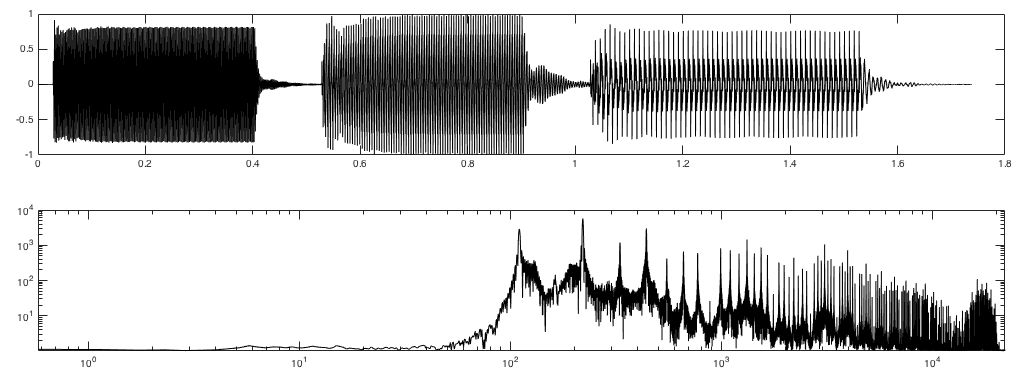
\includegraphics[width=1\textwidth]{bilder/stft01.png}
	\caption[Beispiel für die DFT]{Ein \SI{1.8}{\second} langes Signal. Oben: Der Zeitbereich mit drei klar erkennbaren Tönen. Unten: Das Frequenzspektrum des gesamten Signals mit logarithmierten Achsen.}
	\label{img:stft01}
\end{figure}

Es ist wünschenswert, einen Kompromiss aus den Vorteilen beider Bereiche zu finden, indem man das Spektrum kürzerer Zeitabschnitte des Signals bildet. Hierzu wird der Zeitbereich $x[\;]$ in Fenster der Länge $M$ zerlegt. Die zeitliche Differenz zwischen zwei Fenstern wird als \emph{Hop Size} $R$ bezeichnet. \autoref{eq:signal-Window} definiert die Bildung des \emph{Signalfensters} $x_i[\;]$. Die komplette Zerlegung eines Signals in Signalfenster wird als \emph{Windowing} bezeichnet.\cite{juliusSmith}

\begin{equation}
x_{i}[n] = x[n+i\cdot R]
\label{eq:signal-Window}
\end{equation}

\begin{figure}[h]
	\centering
	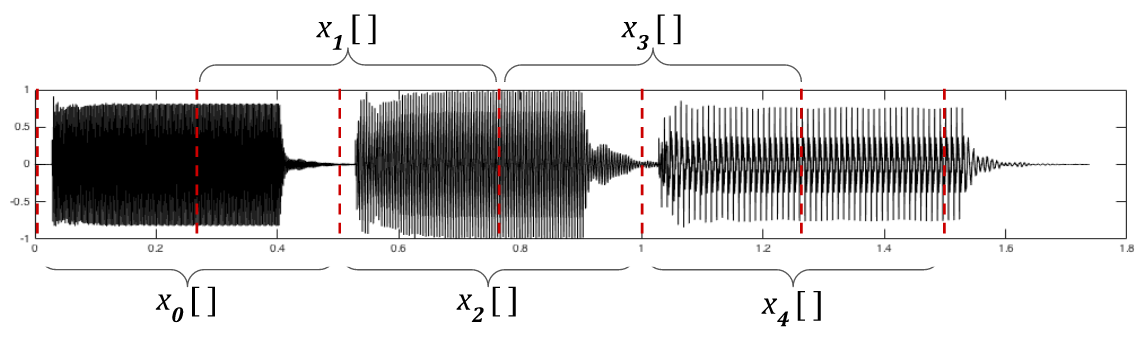
\includegraphics[width=1\textwidth]{bilder/signalWindows02.png}
	\caption{Windowing: Die Zerlegung eines Signals in kürzere Fenster.}
	\label{img:siganlWindows}
\end{figure}

\autoref{img:siganlWindows} zeigt ein Beispiel für die Zerlegung eines Signals $x[\;]$ in die Signalfenster $x_0[\;] ,\ldots, x_4[\;]$. Die Samplingrate des Signals ist $f_s = 44100$, die Fensterlänge beträgt $M = 22050 / f_s = \SI{0.5}{\second}$ und die Hop Size $R = M / 2= \SI{0.25}{\second}$.

Als Vorbereitungsschritt für die Transformation der Signalfenster in den Frequenzbereich wird jedes Signalfenster mit einer \emph{Fensterfunktion} (engl. \emph{window}) $w[\;]$ multipliziert.\cite[S. 69]{sprachverarbeitung} \autoref{eq:hammingWindow} definiert eine der am weitesten verbreiteten Fensterfunktionen, das \emph{Hamming-Window}. Der Paramter $M$ gibt die Länge des Fensters an. \autoref{img:hamming} visualisiert das Hamming-Window.\cite[S. 286]{dspGuide}

\begin{equation}
w[n] = 0.54 - 0.46 \cos(\frac{2\pi n}{M} )
\label{eq:hammingWindow}
\end{equation}

\begin{figure}[h]
	\centering
	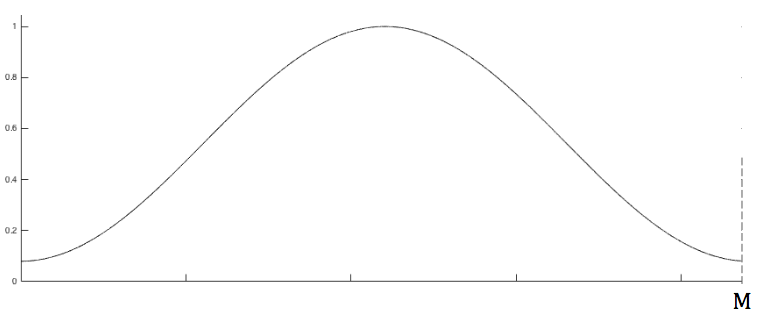
\includegraphics[width=0.5\textwidth]{bilder/hamming01.png}
	\caption{Das Hamming-Window}
	\label{img:hamming}
\end{figure}

\autoref{eq:stft} definiert die \emph{Kurzzeit-Fourier-Transformation} (engl. \emph{Short Time Fourier Transformation}, kurz \emph{STFT}), implementiert mit Hilfe der DFT. Dabei wird das Signalfenster $x_i[\;] = x[n+i\cdot R]$ mit der Fensterfunktion $w[\;]$ multipliziert und in das \emph{Frequenz-Fenster} $X_i[\;]$ transformiert.\cite[S. 69]{sprachverarbeitung} \cite{stft} \autoref{img:stft02} visualisiert die STFT des Beispielsignals aus \autoref{img:siganlWindows}.

\begin{equation}
X_i[k] = \sum_{n=0}^{M-1} x[n+i\cdot R] \cdot w[n] \cdot e^{-j 2\pi k \frac{n}{N}}
\label{eq:stft}
\end{equation}

\begin{figure}[h]
	\centering
	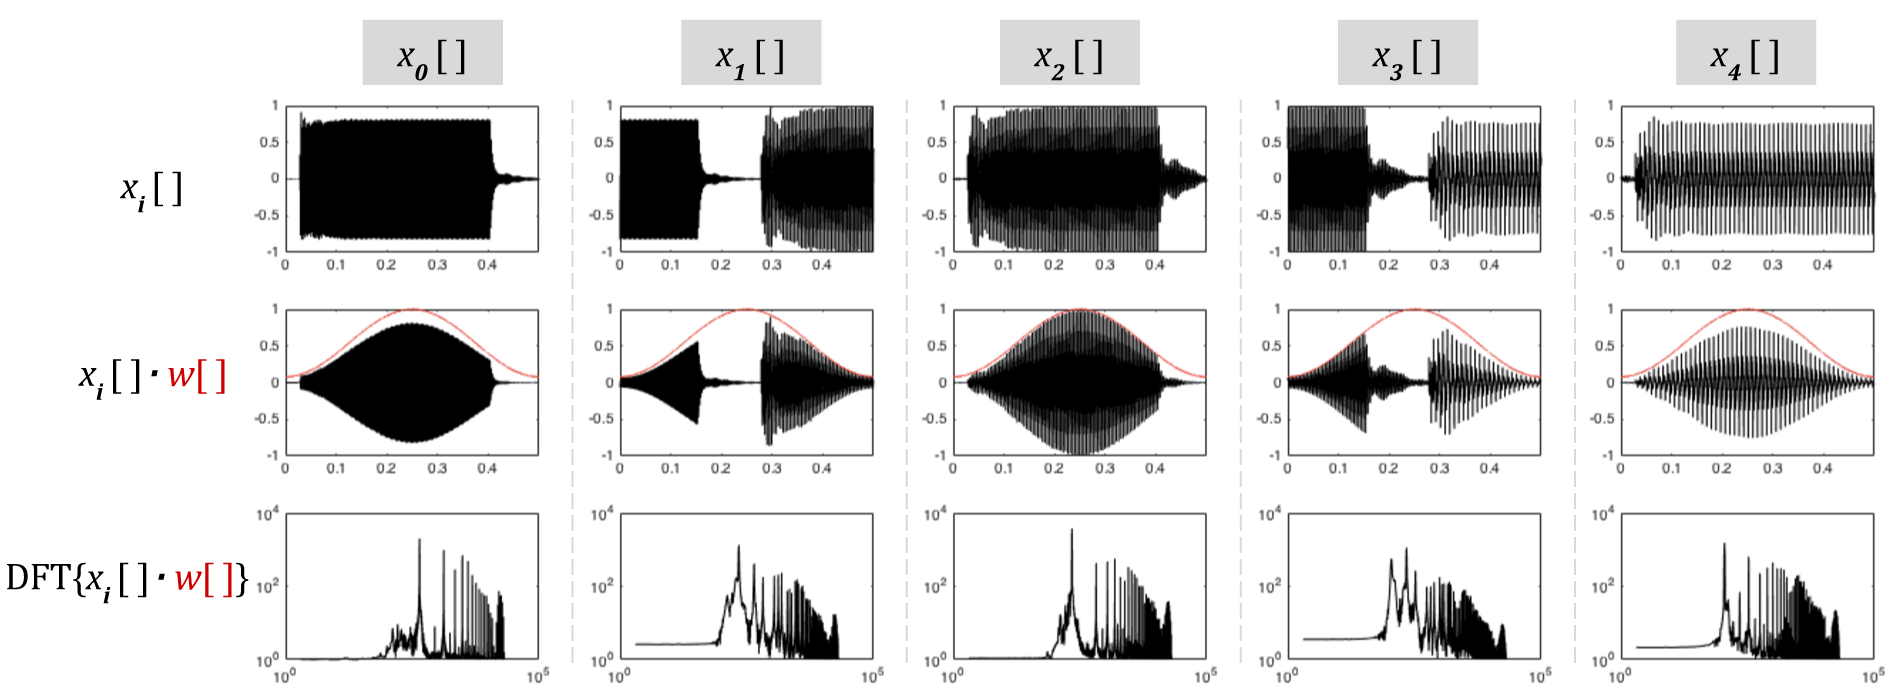
\includegraphics[width=1\textwidth]{bilder/signalWindows03.png}
	\caption{STFT des Beispielsignals aus \autoref{img:siganlWindows}}
	\label{img:stft02}
\end{figure}

\pagebreak

\subsection{Akustische Modellierung der menschlichen Stimme}
\label{sec:theVoice}

Der menschliche Sprechapparat wird in die folgenden Komponenten unterteilt:

\begin{description}

\item[Schallproduktion: ] Die Lunge stößt Luft aus, welche die Stimmbänder passiert. Sind die Stimmbänder leicht gespannt, so wird der Luftstrom periodisch unterbrochen. Die Schwingfrequenz beträgt bei erwachsenen Männern etwa \SI{120}{\hertz} und bei Frauen \SI{220}{\hertz}. Die Frequenz kann während des Sprechens um bis zu einer Oktave variieren. So wird ein periodisches Signal produziert, bezeichnet als \emph{Periodische Quelle} (engl. \emph{Periodic Source}). Sind die Stimmbänder stark gespannt, so entstehen Turbulenzen, die sich akustisch als ein zischendes Geräusch ohne identifizierbare Tonhöhe äußern. Dieses stimmlose Signal wird bezeichnet als \emph{Turbulenzquelle} (engl. \emph{Turbulence Source})
\item[Klangformung: ] Das Signal der Stimmlippen passiert den Rachen, Mund- und Nasenraum, welche gemeinsam als \emph {Vokaltrakt} bezeichnet werden. Das Halszäpfchen bestimmt, ob der Luftstrom in den Mund- oder Nasenraum geleitet wird. Die Stellung der Artikulatoren, bestehend aus dem Kiefer, der Zunge usw. bestimmen die Beeinflussung des Klangs des Signals, das durch die Stimmbänder erzeugt wird. Diese Beeinflussung wird als lineares, zeitinvariantes Filter angenähert.\cite[S. 62]{cryModel} \cite[S. 13]{sprachverarbeitung} \autoref{img:schematicVocalOrgans} visualisiert diese Komponenten.
\end{description}

\begin{figure}[h]
	\centering
	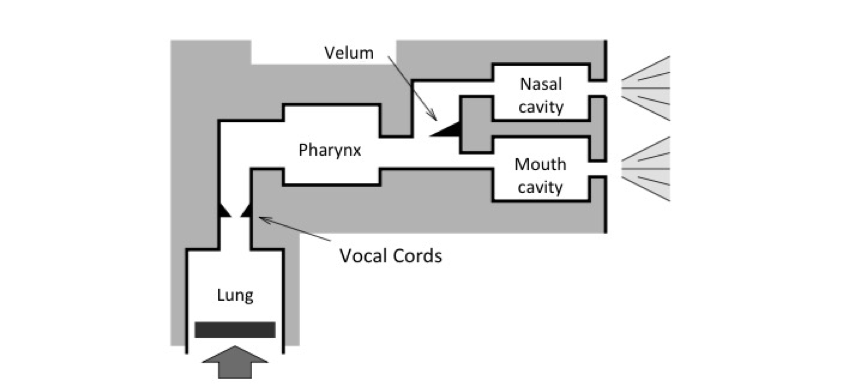
\includegraphics[width=0.7\textwidth]{bilder/SchematicVocalOrgans.png}
	\caption[Schematische Übersicht über die Organe des Sprechapparates]{Schematische Übersicht über die Organe des Sprechapparates. Lung = Lunge, Vocal Chords = Stimmbänder, Pharynx = Rachen, Velum = Halszäpfchen, Mouth Cavity = Mundraum, Nasal Cavity = Nasenraum \cite{speechProduction}}
	\label{img:schematicVocalOrgans}
\end{figure}	

In der Signalverarbeitung wird die menschliche Lautproduktion durch das sogenannte \emph{Source-Filter-Modell} modelliert. Der durch die Stimmbänder erzeugte, periodische Ton wird angenähert durch einen Impuls-Zug, welcher durch den Schlund als lineares Filter moduliert wird. Das stimmlose, nicht-periodische Signal wird durch weißes Rauschen angenähert. Der periodische oder nicht-periodische Ton wird als das Eingangssignal $u[\;]$ bezeichnet. Dieses Signal wird an den Vokaltrakt weitergeben, welcher als lineares, zeitinvariantes Filter mit der Impulsantwort $v[\;]$ modelliert wird. Diese Impulsantwort ist abhängig von der Konfiguration der Organe des Vokaltraktes. Die Lippen werden als zweites lineares, zeitinvariantes Filter mit der Impulsantwort $r[\;]$ modelliert. $r[\;]$ wird auch als \emph{Radiant Model} bezeichnet. Das tatsächliche Sprachsignal $y[\;]$ entsteht somit durch die Faltung des Signals $u[\;]$ mit den beiden linearen, zeitinvarianten Filtern nach \autoref{eq:source-Filter-Model}. \autoref{eq:source-Filter-Model2} definiert den Frequenzbereich des Ausgangssignals $Y[\;]$ durch die Multiplikation der Frequenzbereiche der drei Komponenten.\cite[S. 62 - 63]{cryModel} \cite{speechProduction} \autoref{img:source-filter-model} visualisiert diesen Prozess schematisch.

\begin{equation}
u[\;] * v[\;] * r[\;] = y[\;] 
\label{eq:source-Filter-Model}
\end{equation}

\begin{equation}
U[\;] \cdot V[\;] \cdot R[\;] = Y[\;] 
\label{eq:source-Filter-Model2}
\end{equation}

\begin{figure}[H]
	\centering
	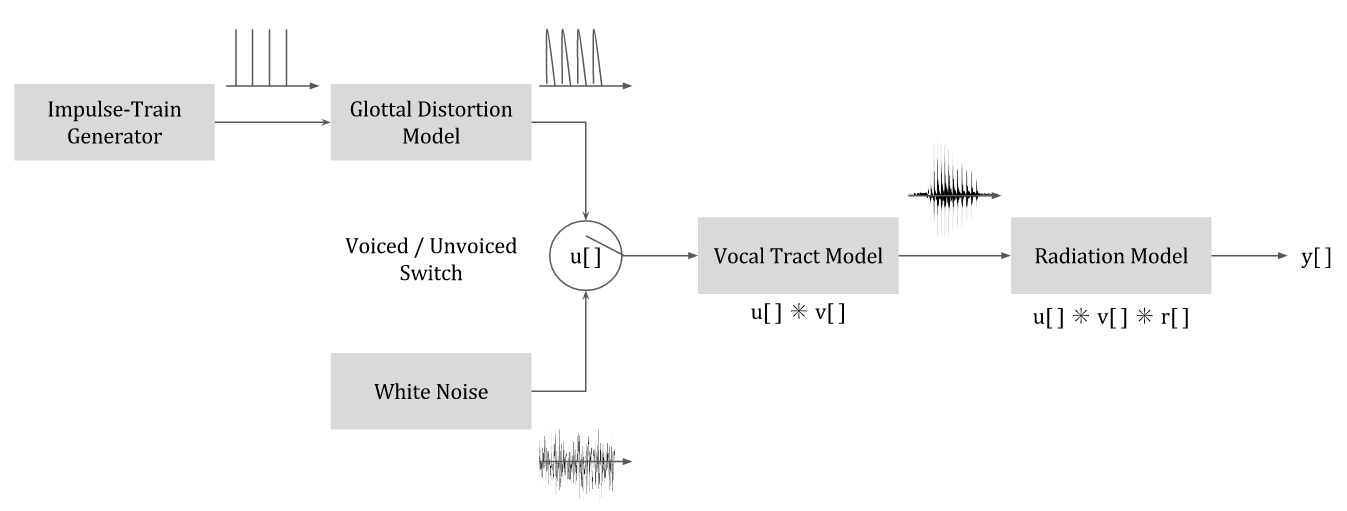
\includegraphics[width=1\textwidth]{bilder/source-filter-model.png}
	\caption[Schematische Übersicht über das Source-Filter-Modell]{Schematische Übersicht über das Source-Filter-Modell (nach: \cite[ \emph{Source estimation}, S. 17]{ricardo_ceps})}
	\label{img:source-filter-model}
\end{figure}	

\autoref{img:glottalSource} zeigt die Zeitbereiche der stimmhaften und der turbulenten Quelle im Vergleich. Wie zu sehen ist, bestimmt der zeitliche Abstand zwischen den Impulsen die Grundfrequenz der Stimme. Dieses Signal $p[\;]$ wird durch den Schlund als Filter $G\{ \; \}$ gefiltert, wodurch der Zeitbereich der periodischen Quelle $G\{p[\;]\} = u_p[\;]$ entsteht. Darunter ist der Zeitbereich des weißen Rauschen zu sehen.\cite[\emph{Source}]{speechAcoustics}

\begin{figure}[h]
	\centering
	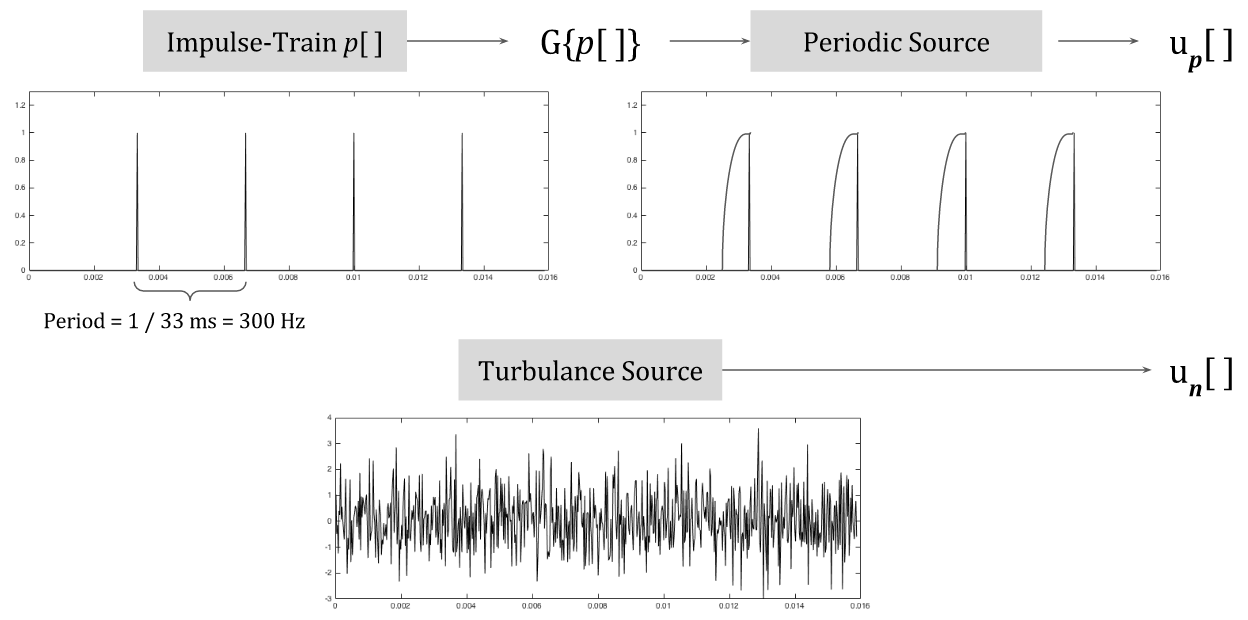
\includegraphics[width=1\textwidth]{bilder/glottalSource.png}
	\caption[Zeitbereiche der periodischen und der turbulenten Quelle]{Zeitbereiche der periodischen und der turbulenten Quelle (nach: \cite[Source]{speechAcoustics})}
	\label{img:glottalSource}
\end{figure}	

\autoref{img:sourceFilerSpectra} zeigt die Frequenzbereiche der Komponenten des Source-Filter-Modells. Die periodische Quelle ($U[\;]$ links) zeichnet sich im Frequenzbereich durch gleichmäßig verteilte Spitzen aus, die mit steigender Frequenz an Amplitude verlieren. Rechts daneben ist der Frequenzbereich des weißen Rauschen zu sehen, welcher einer Zufallsverteilung entspricht. Die Frequenzantwort des Vokaltraktes $V[\;]$ zeichnet sich durch Resonanzfrequenzen aus, von denen in diesem Beispiel vier  erkennbar sind. Die Übertragungsfunktion der Lippen $R[\;]$ wird als Hochpassfilter angenähert. Das Ausgangssignal $Y[\;] = U[\;] \cdot V[\;] \cdot R[\;]$ zeigt den Einfluss der Filter auf das jeweilige Eingangssignal.\cite[\emph{Source estimation}]{ricardo_ceps}, \cite[\emph{Vocal Tract Resonance}]{speechAcoustics}

\begin{figure}[h]
	\centering
	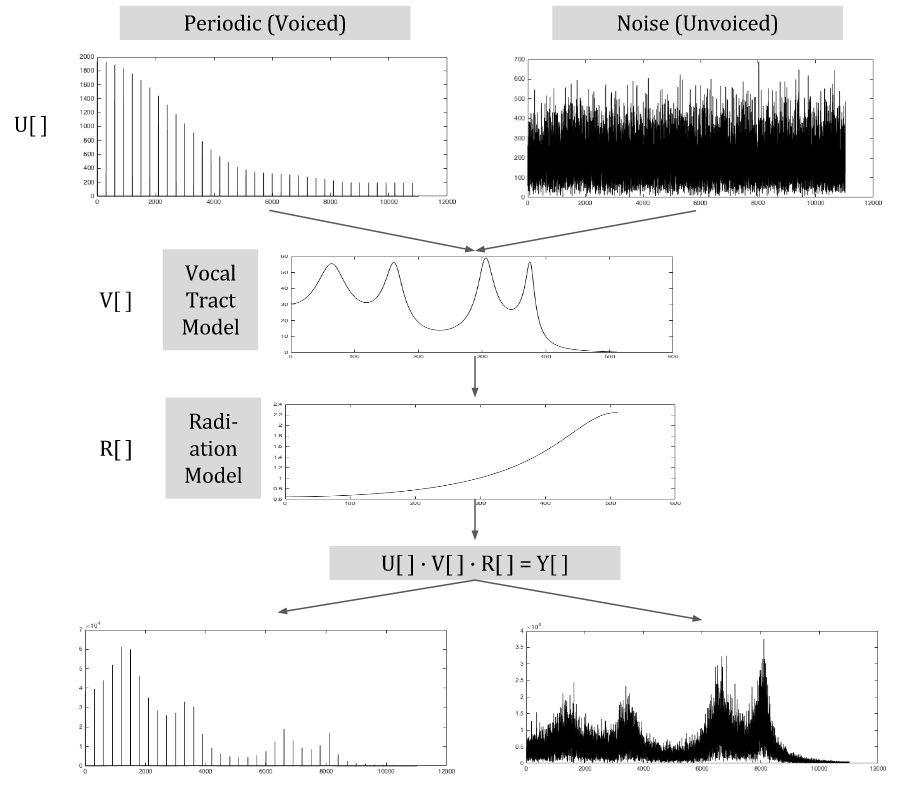
\includegraphics[width=1\textwidth]{bilder/sourceFilterSpectra.png}
	\caption[Betrachtung der Frequenzbereiche des Source-Filter-Modells]{Betrachtung der Frequenzbereiche des Source-Filter-Modell (nach: \cite[\emph{Source Estimation}, S. 3]{ricardo_ceps})}
	\label{img:sourceFilerSpectra}
\end{figure}	

\autoref{img:pitchPeaks} zeigt schematisch das Spektrum eines stimmhaften Sprachsignals. Sowohl die \emph{Grundfrequenz} (engl. \emph{Fundamental Frequency}) als auch die harmonischen Obertonwellen (engl. \emph{Harmonics}) sind rein visuell als \glqq viele, kurze Signalspitzen\grqq{} im Spektrum erkennbar. Der kleinste gemeinsame Teiler der Frequenzen dieser Signalspitzen entspricht der Grundfrequenz $f_0$ des Stimmsignals, in diesem Beispiel $\SI{250.7}{\hertz}$. Die Grundfrequenz ist ebenfalls an der Signalspitze mit der tiefsten Frequenz ablesbar. Die harmonischen Obertöne entsprechen der doppelten, dreifachen,$\ldots\ $ Grundfrequenz, das heißt $2\cdot f_0, 3\cdot f_0, \ldots$ und werden bezeichnet mit $H_1, H_2, \ldots$. Die Grundfrequenz ist \emph{nicht zwingend} die Spitze mit der höchsten Amplitude. Durch den Einfluss des Vokaltraktes als Filter können harmonische Obertöne eine höhere Amplitude als die Grundfrequenz erhalten. Mit Hilfe des Frequenzspektrums lässt sich somit visuell ein stimmhaftes Signal von einem nicht stimmhaften Signal unterscheiden, indem das Spektrum nach dem Vorhandensein regelmäßiger Signalspitzen überprüft wird (vergleiche mit \autoref{img:sourceFilerSpectra}).\cite[S. 52 - 53]{sprachverarbeitung}

% To do: Quelle!!
\begin{figure}[h]
	\centering
	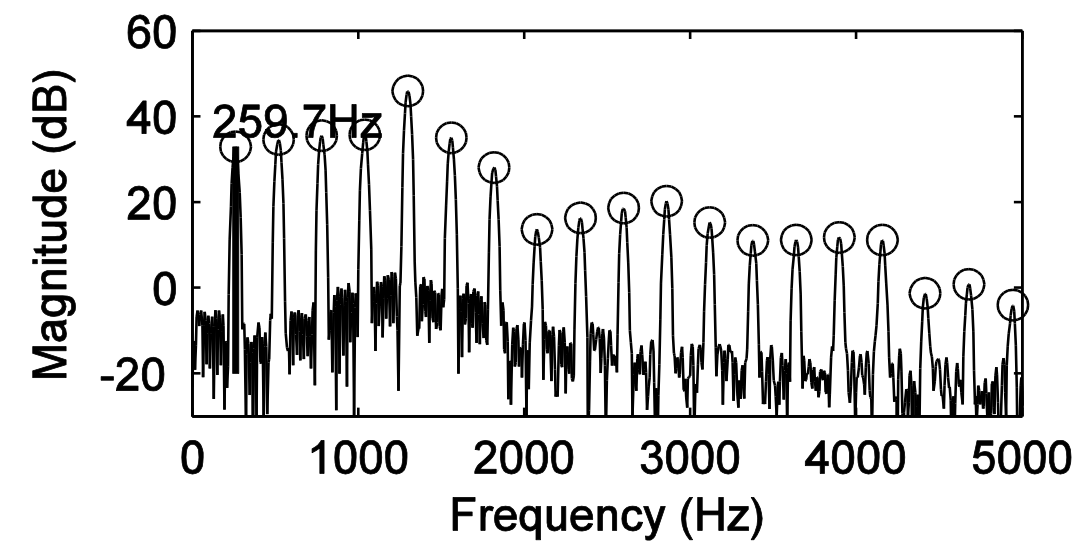
\includegraphics[width=0.5\textwidth]{bilder/pitchPeaks.png}
	\caption[Grundfrequenz und harmonische Obertöne eines stimmhaften Sprachsignals]{Grundfrequenz und harmonische Obertöne eines stimmhaften Sprachsignals \cite{onePitchImage}}
	\label{img:pitchPeaks}
\end{figure}	

\autoref{img:formants} verdeutlicht, wie der als lineares, zeitinvariantes Filter modellierte Vokaltrakt durch Formanten bestimmt wird. Diese Formanten spielen vor allem bei der Beschreibung von Vokalen eine Rolle. Formanten sind lokale Maxima im Spektrum der Transferfunktion, die durch Resonanzen im Vokaltrakt erzeugt werden. Ein Formant wird durch seine Mittenfrequenz, seine Bandbreite und seine Amplitude beschrieben. Die Formanten einer Vokaltraktkonfiguration werden der Reihenfolge ihrer Mittenfrequenzen entsprechend nach dem Schema $F_1 , \ldots , F_n$ nummeriert.  Mit steigender Frequenz nimmt die Amplitude der Formanten ab, der dominanteste Formant ist somit immer der erste. Daher werden meist nur die ersten zwei oder drei Formanten zur Beschreibung eines Vokals angegeben, auch, wenn theoretisch weitaus mehr vom Vokaltrakt erzeugt werden. Für verschiedene Sprachen sind allerlei Tabellen zu finden, welche die Formantenfrequenzen der Vokale auflisten.\cite[S. 19]{sprachverarbeitung}

\begin{figure}[h]
	\centering
	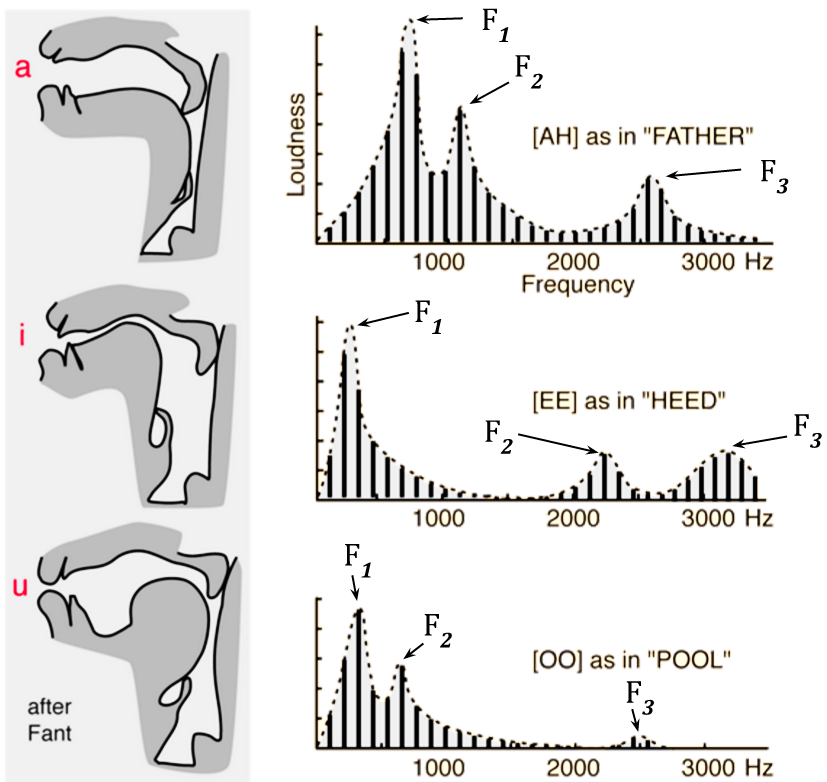
\includegraphics[width=0.55\textwidth]{bilder/formants03.png}
	\caption[Beispiele für Formanten im Sprachsignal]{Beispiele für Formanten im Sprachsignal (nach: \cite{benade})}
	\label{img:formants}
\end{figure}

Beim Sprechen befinden sich sowohl das Signal der Stimmbänder als auch das Filter des Vokaltraktes und der Lippen in ständiger Veränderung. Ein stimmhaftes Sprachsignal gilt nur über kurze Zeitbereiche weniger Millisekunden als periodisch, und selbst in diesen kurzen Zeitbereichen ist die Stimme nicht perfekt, sondern nur annähernd periodisch. Da die Informationen der Sprache vor allem im Frequenzbereich codiert sind, wird die in \autoref{sec:stft} vorgestellte Kurzzeit-Fourier-Transformation zur Analyse von Sprache eingesetzt. Die Visualisierung der Kurzzeit-Fourier-Transformation wird als \emph{Spektogramm} bezeichnet. Dabei werden auf der x-Achse die Zeitpunkte der Fenster und auf der y-Achse die Frequenzen dargestellt. Die Frequenzfenster werden \glqq auf die Seite gelegt\grqq{}, damit der zeitliche Verlauf übersichtlich betrachtet werden kann. Die Amplitude der entsprechenden Frequenzen wird farblich oder durch Helligkeiten codiert, abhängig von der konkreten Implementierung des Spektogramms. Je länger das Zeitfenster der STFT, desto höher ist die Auflösung des Frequenzbereiches und desto niedriger die Auflösung des Zeitbereiches. Je kürzer die Zeitfenster der STFT, desto höher ist die Auflösung des Zeitbereiches, und desto niedriger die Auflösung des Frequenzbereiches.\cite[S. 45 - 50]{sprachverarbeitung} \cite[\emph{Acoustic Representations of Speech}]{speechAcoustics}.

\autoref{img:spectoExample} zeigt ein Beispiel für zwei Spektogramme mit unterschiedlichen Fensterlängen der STFT, angewandt auf einer 9 Sekunden langen Aufnahme eines weinenden Babys. Es ist zu erkennen, dass bei der geringeren Fensterlänge der zeitliche Verlauf besser erkennbar ist, jedoch die einzelnen harmonischen Obertöne weniger gut voneinander unterscheidbar sind. Bei der längeren Fensterlänge sind die Formanten leichter zu unterscheiden, die Anfangs- und Endzeitpunkte der Lautäußerungen sind jedoch schwerer zu lokalisieren.

\begin{figure}[H]
	\centering
	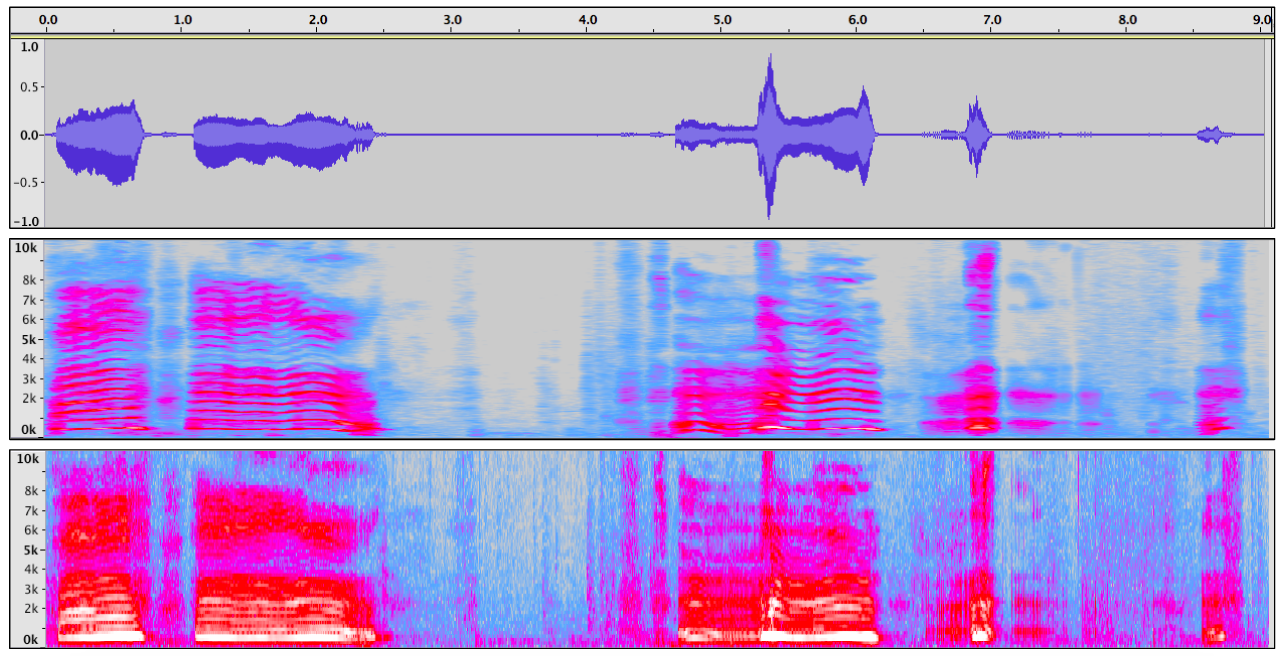
\includegraphics[width=1\textwidth]{bilder/spectogram03.png}
	\caption[Spektogramm einer Audioaufnahme eines Babys]{Oben: Zeitbereich einer Audioaufnahme eines weinenden Babys. Mitte: Spektogramm mit einer Fensterlänge von $\SI{185}{\milli\second}$ (8192-Sample DFT). Unten: Spektogramm mit einer Fensterlänge von $\SI{5}{\milli\second}$ (265-Sample DFT). Rot entspricht hohen Amplituden, Blau entspricht niedrigen Amplituden. (Abbildung erzeugt mit dem Programm \glqq Audacity\grqq)}
	\label{img:spectoExample}
\end{figure}	

\section{Schmerz und Weinen bei Neugeborenen}
\label{sec:medicalFoundations} 

Schmerz wird definiert als ein \glqq unangenehmes Sinnes- oder Gefühlserlebnis, das mit tatsächlicher oder potenzieller Gewebeschädigung einhergeht\grqq{}.\cite[S. 438]{PainAssessment01} In der ersten Hälfte des 20. Jahrhunderts war die vorherrschende Meinung, dass Neugeborene keinen Schmerz empfinden können, wodurch sie beispielsweise nach Operationen häufig keine Schmerzmittel verabreicht bekamen. Der aktuelle Stand der Forschung ist, dass Neugeborene im ähnlichen Maße wie Erwachsene Schmerz empfinden können. Die freien Nervenenden, die in der Lage sind, physische Schäden am Körper festzustellen, sind bei Neugeborenen ebenso wie bei Erwachsenen über den Körper verteilt. Die hormonelle Reaktion ist ebenfalls vergleichbar.\cite[S. 402]{PainAssessment03} \cite[S. 438]{PainAssessment01}

\subsection{Schmerz-Scales als Instrumente zur Schmerzbewertung}
\label{sec:painScores}

%besseres wort als Gründe!
Schmerz kann durch diverse Ursachen bei Neugeborenen ausgelöst werden. Diese reichen von physischen Schäden, beispielsweise aufgrund von Komplikationen bei der Geburt oder Gewalteinwirkungen, über Erkrankungen, wie Kopfschmerzen oder Infektionen, bis hin zu therapeutischen Prozeduren, wie Injektionen oder der Desinfektion von Wunden. Das Vorhandensein von Schmerz ist anhand verschiedener physiologischer, biochemischer, verhaltensbezogener und psychologischer Veränderungen erkennbar.\cite[S. 438]{PainAssessment01} Ein Merkmal, welches das Vorhandensein von Schmerz anzeigt, wird als \emph{Schmerzindikator} bezeichnet. Abbildung \ref{img:painIndicators} zeigt einen Überblick über einige Schmerzindikatoren. Ein Beispiel für einen Schmerzindikator ist der \emph{Gesichtsausdruck} (engl. \emph{Facial Expression}). Schmerzindikatoren werden zu sogenannten \emph{Modalitäten} oder \emph{Dimensionen} gruppiert. Ein Beispiel für eine Schmerz-Dimension ist das \emph{Verhalten} (engl. \emph{Behavioral Indicators}). Der Fokus dieser Arbeit liegt auf dem \emph{Weinen}, welches zu den verhaltensbezogenen Indikatoren zählt.\cite[S. 69 - 70, 81]{PainAssessment02} \cite[S. 2]{overview}

\begin{figure}[H]
	\centering
	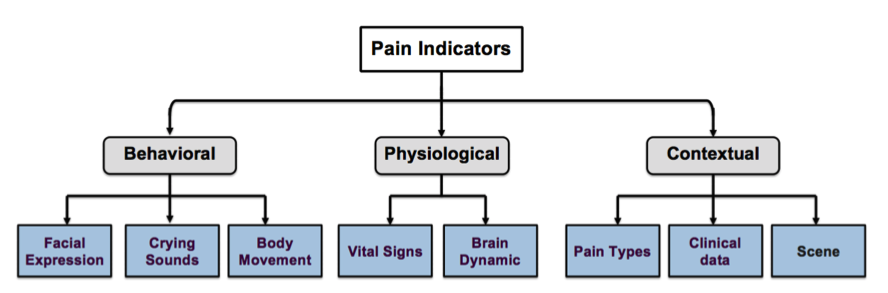
\includegraphics[width=1\textwidth]{bilder/painDimensions.png}
	\caption[Übersicht über Schmerzindikatoren]{Übersicht über eine Auswahl an Schmerzindikatoren \cite[S. 2]{overview}}
	\label{img:painIndicators}
\end{figure}

Schlussendlich ist Schmerz eine subjektive Empfindung. Das heißt, dass ein und der selbe Stimulus bei zwei verschiedenen Personen zu einem unterschiedlichen Schmerzempfinden führen kann. Daher wird der Schmerzgrad bei Erwachsenen typischerweise durch eine Selbsteinschätzung des Patienten unter der Leitung des Arztes festgestellt. Bei Kindern unter drei Jahren ist diese Selbsteinschätzung nicht möglich. Die Schmerzbewertung muss daher von anderen Personen vorgenommen werden. Im klinischen Kontext sind dies medizinische Fachkräfte, wie beispielsweise Ärzte, Krankenpfleger oder Geburtshelfer. Die von außen am leichtesten feststellbaren Indikatoren von Schmerz sind verhaltensbasierte Merkmale. Die Schmerzdiagnostik durch eine andere Person ist, genau wie das Schmerzempfinden, etwas inherent subjektives und abhängig von Faktoren wie dem Alter, Geschlecht, kulturellen Hintergrund, persönlichen Erfahrungen mit Schmerz usw.\cite[S. 1 - 3]{overview} \cite[S. 438]{PainAssessment01} Um die Schmerzdiagnostik objektiver zu gestalten, wurden daher sogenannte \emph{Schmerz-Scales} (engl. \emph{Pain-Scales}) entwickelt, welche mit Hilfe eines Punktesystems den Schmerzgrad des Babys quantifizieren.\cite[S. 240]{painAssessmentStatus} Es existieren \emph{unidimensionale} (auch bezeichnet als \emph{unimodale}) Schmerz-Scales, bei denen der Schmerzgrad aus der Beobachtung \emph{eines} Schmerzindikators, wie beispielsweise dem Gesichtsausdruck, geschlossen wird. \emph{Multidimensionale} (auch bezeichnet als \emph{multimodale}) Schmerz-Scales beziehen mehrere Schmerzindikatoren verschiedener Dimensionen in die Schmerzbewertung mit ein. Solche Schmerz-Scales, die mehrere Schmerzindikatoren einer Dimension bewerten, also beispielsweise nur verhaltensbezogene Schmerzindikatoren, werden je nach Quelle zu den unimodalen oder den multimodalen Schmerz-Scales gezählt. In dieser Arbeit sind mit multimodalen Schmerz-Scales solche gemeint, die unabhängig von der Dimensionalität unterschiedliche Schmerzindikatoren für die Schmerzbewertung verwenden. Die vorgestellten Konzepte lassen sich jedoch uneingeschränkt anwenden, auch wenn man für eine Multimodalität Schmerzindikatoren verschiedener Dimensionen voraussetzt.\cite[S. 68 - 69, 80 - 81]{PainAssessment02} \cite[S. 1-2, 31]{overview} \cite[S. 404]{PainAssessment03} 

\autoref{tab:nips} zeigt die \glqq Neonatal Infant Pain Scale\grqq{} (NIPS) als Beispiel für eine multimodale Schmerz-Scale. Sie ist für Babys von 0 bis 1 Jahr geeignet und vor allem für die Diagnose von Schmerz gedacht, der während einer Prozedur entsteht. Die Scale wurde auf der Basis der Erfahrungen von Krankenschwestern erarbeitet. Das Baby soll bei der Anwendung dieser Schmerz-Scale für ungefähr eine Minute beobachtet werden. Soll der Schmerz nach einem Eingriff überwacht werden, wird empfohlen, die Diagnose so lange alle 30 Minuten durchzuführen, bis kein Schmerz mehr festgestellt wird. Für jede der aufgeführten Kategorien (Schmerzindikatoren) wird ein \emph{Score} von ein, zwei oder drei Punkte vergeben. Die Scores aller Kategorien werden daraufhin aufaddiert und ergeben den insgesamten \emph{Schmerz-Score} (engl. \emph{Pain-Score}), welcher anschließend interpretiert wird. Bei der NIPS steht ein Schmerz-Score von $>3$ für \glqq moderaten Schmerz\grqq , ein Score von $>4$ für \glqq großen Schmerz\grqq.\cite{nips} \cite[S. 98]{painInNeonates}

\begin{table}[h]

	\centering
	\caption[Neonatal Infant Pain Scale]{Neonatal Infant Pain Scale (NIPS) \cite{nips}}
	\label{tab:nips}
	\begin{tabular}{@{}cccc@{}}
		\toprule
		\textbf{Indicator}     & \textbf{0 points} & \textbf{1 point}     & \textbf{2 points} \\ \midrule
		Facial Expr. & Relaxed           & Contracted           & -                 \\
		Cry               & Absent            & Mumbling             & Vigorous          \\
		Breathing         & Relaxed           & Different than basal & -                 \\
		Arms              & Relaxed           & flexed/stretched     & -                 \\
		Legs              & Relaxed           & flexed/stretched     & -                 \\
		Alertness         & Sleeping          & uncomfortable        & -                 \\ \bottomrule
	\end{tabular}
\end{table}


Es wurden viele weitere multimodale Schmerz-Scales entwickelt, die grundlegend dem Schema der NIPS ähneln. Sie unterscheiden sich hinsichtlich der Schmerzindikatoren, die betrachtet werden, dem Scoring-System, der Art des zu diagnostizierenden Schmerzes, dem Beobachtungszeitraum usw. Einige Schmerz-Scales sind beispielsweise auf die Schmerzdiagnostik während eines Eingriffes spezialisiert, andere auf den darauf folgenden Heilungsprozess. Das Vorgehen zur Schmerzbewertung mit Schmerz-Scales lässt sich folgendermaßen verallgemeinern:

\begin{enumerate}
\item Es wird für jeden Indikator der Schmerz-Scale ein Score nach den angegebenen Kritierien vergeben.
\item Alle Scores werden aufsummiert und ergeben einen insgesamten Schmerz-Score.
\item Der Schmerz-Score wird nach einem von der Schmerz-Scale vorgegebenem Schema interpretiert.\cite{aboutKids}\cite{pat}
\end{enumerate}

In den meisten multimodalen Schmerz-Scales wird das \emph{Weinen} oder \emph{Schreien} (engl. \emph{Cry}) des Babys als Schmerzindikator mit einbezogen.\cite[S. 97 - 98]{painInNeonates} Obwohl Weinen oder Schreien im Deutschen eine negative Konnotation tragen kann, ist in dieser Arbeit mit diesen Begriffen im allgemeinen eine \glqq kindliche Lautäußerung\grqq{} gemeint. 

\autoref{tab:painscores} auf Seite \pageref{tab:painscores} zeigt eine Übersicht über weitere multimodale Schmerz-Scales. Es sind nur solche Scales enthalten, die das Weinen als Schmerzindikator mit einbeziehen. Für jede Schmerz-Scale wird gezeigt, nach welchen Kriterien das Scoring für das Weinen vorgenommen wird. Ebenfalls werden die weiteren Schmerzindikatoren gelistet, die von der jeweiligen Schmerz-Scale mit einbezogen werden, ohne die Scoring-Systeme für diese Indikatoren detailliert wiederzugeben. Darüber hinaus wird für jede Schmerz-Scale angegeben, für welches Alter und welchen Schmerz-Typ sie vorgesehen ist. Angaben bezüglich der Diagnosehäufigkeit sowie des jeweiligen Beobachtungszeitraums werden gemacht, insofern sie von einer Scale empfohlen wurden. Die Tabelle ist in Englisch verfasst, da alle Quellen der hier gelisteten Schmerz-Scales dem Autor in Englisch vorliegen.

Da die Begriffe \emph{Schmerz-Scale} und \emph{Schmerz-Score} in einigen Veröffentlichungen inkonsistent verwendet werden, wird  darauf hingewiesen, dass mit \emph{Schmerz-Scale} das System zur Schmerzdiangostik gemeint ist und mit \emph{Schmerz-Score} die auf Basis der Schmerz-Scale vergebene Punktzahl. Die folgenden Bemerkungen werden weiterhin bezüglich der Schmerz-Scales aus \autoref{tab:painscores} gemacht:

\begin{itemize}
	
	\item Bei den Schmerz-Scale handelt es sich sowohl bei den Scorings der einzelnen Kategorien als auch bei den Schmerz-Scores um Ordinalskalen. Das bedeutet beispielsweise, dass bei einer Schmerz-Scale ein Schmerz-Score von 4 einen stärkeren Schmerz anzeigt als ein Score von 2, daraus aber nicht geschlossen werden kann, dass der Schmerz doppelt so stark ist. Daraus ergibt sich ebenfalls, dass sowohl die Schmerz-Scores als auch die kategorienbezogenen Scorings verschiedener Schmerz-Scales nicht untereinandet vergleichbar sind. So wird der höchst mögliche Schmerz-Score beispielsweise bei der NIPS mit 7 \cite{nips}, bei der FLACC mit 10 \cite{flacc} und bei der PAT mit 20 \cite{pat} definiert. Ein Schmerz-Score lässt sich folglich nur bei Kenntnis der verwendeten Schmerz-Scale interpretieren.
	\item Ein Teil der aufgelisteten Schmerz-Scales ist für die Schmerzbeurteilung während einer Prozedur gedacht. Die Schmerz-Scales, die zur Bewertung von post-operativen oder andauernden (engl. \emph{ongoing}) Schmerzen geeignet sind, nennen in den jeweiligen Anwendungsvorschriften gewisse Diagnosehäufigkeiten. Beispielsweise empfiehlt die PAT-Scale, die Diagnose nach einer Operation stündlich durchzuführen, bis sich der Gesundheitszustand stabilisiert hat. Anschließend sollte eine Schmerzdiagnose alle 4 Stunden stattfinden.\cite{pat} N-PASS empfiehlt nach Operationen eine Diagnose alle 2 bis 4 Stunden.\cite{flacc} Einige Schmerz-Scales definieren informellere Diagnosefrequenzen, sowie die COMFORT-Scale, welche eine Diagnose vorsieht, wenn \glqq Schmerz vermutet wird\grqq{}, direkt vor und 30 Minuten nach einer Medikation, sowie zu Beginn jedes Schichtwechsels.\cite[S. 241]{painAssessmentStatus}
	
	\item Bei Schmerz-Scales, welche für die Schmerzbeurteilung von Prozeduren gedacht sind, bedingt der Zeitraum der Prozedur den Zeitraum der Schmerzbewertung. Von den Scales, die für andauernde Schmerzen und für die post-operative Begutachtung vorgesehen sind, definieren einige konkret, wie lange das Baby für die Diagnose beobachtet werden soll, um den Schmerz-Score festzulegen. Die PAT empfiehlt eine Beobachtung von 15 bis 30 Sekunden \cite{pat}, FLACC 1 bis 5 Minuten bei wachen und mehr als 5 Minuten bei schlafenden Patienten.\cite{flacc} Schmerz-Scales, die keine festen Beobachtungszeiträume festlegen, implizieren diese durch die Kriterien der Schmerzbewertung. Die FLACC beispielsweise bewertet ein Weinen mit einem Score von 2, wenn es \glqq stetig\grqq{} ist und DAN vergibt einen Score von 2 für \glqq lang anhaltendes Weinen\grqq. \cite{flacc} Die BPSN schließt den Schmerzgrad vor Allem aus der Länge des Weinens.\cite{bpsn} Die nicht explizite Definition der Beobachtungszeiträume stellt eine Schwierigkeit bei Schmerz-Scales dar, da sie die Vergleichbarkeit der Bewertungsergebnisse verschiedener diagnostizierender Personen mindert.\cite[S. 100]{painInNeonates}
	
	\item Die Kriterien zum Scoring des Weinens werden zum größten Teil mit \emph{subjektiv behafteten Begriffen} beschrieben. Beispielsweise wird bei dem \emph{N-PASS}-System ein Score von drei für \glqq High-pitched or silent-continuous crying\grqq{} vergeben. Die Begriffe \glqq high-pitched\grqq{} und \glqq silent-continuous\grqq{} werden nicht näher definiert. Auch die Anwendungsvorschriften der Schmerz-Scales geben keine festen Definitionen. Dies erleichtert den praktischen Einsatz der Scales, führt jedoch zu einem Interpretationsspielraum und somit zu einem von der diagnostizierenden Person abhängigen Scoring. Die \emph{BPSN}-Scale nutzt als einzige der vorgestellten Scales objektiv messbare Eigenschaften in Bezug auf das Weinen.
	
	%\item Die Schmerz-Scales fokussieren unterschiedliche Eigenschaften für das Scoring bezüglich des Weinens. Bei \emph{CRIES} ist die Tonhöhe, bei \emph{BPSN} die Länge und bei \emph{COMFORT} die Art des Weinens ausschlaggebend für die Höhe des vergebenen Scores.
	
\end{itemize}

\pagebreak

\vspace{-3mm}
\footnotesize
\begin{longtable}{@{}lllll@{}}
	\caption[Übersicht über die Bewertung des Weinens verschiedener multimodaler Schmerz-Scales]{Übersicht über die Bewertung des Weinens verschiedener multimodaler Schmerz-Scales \cite[S. 98 ]{painInNeonates} \cite{flacc} \cite{npass} \cite{bpsn} \cite{cries} \cite{covers} \cite{pat} \cite{dan} \cite{comfort} \cite{bpsn} \cite[S. 71, 75]{PainAssessment02} } \\
\toprule
\textbf{System} & \textbf{S.} & \textbf{Beschreibung des Weinens}                                                                                                                 & \textbf{weitere Indikat.}                                                                                              & \textbf{Sonstiges}                                                                         \\ \midrule
FLACC           & 0           & No cry (awake or asleep)                                                                                                             & \multirow{3}{*}{\begin{tabular}[c]{@{}l@{}}Face, \\ Legs, \\ Activity,\\ Consolability\end{tabular}}             & Age: 2 months - 7 years                                                                   \\
& 1           & \begin{tabular}[c]{@{}l@{}}Moans or whimpers; \\ occasional complaint\end{tabular}                                                   &                                                                                                                  & \begin{tabular}[c]{@{}l@{}}Pain-Type: Ongoing \end{tabular}     \\
& 2           & \begin{tabular}[c]{@{}l@{}}Crying steadily, screams or sobs, \\ frequent complaints\end{tabular}                                     &                                                                                                                  & Observe for: 1 - 5 minutes                                                                        \\ \midrule
N-PASS          & -2          & No cry with painful stimuli                                                                                                           & \multirow{4}{*}{\begin{tabular}[c]{@{}l@{}}Behaviour,\\ Facial Expr.,\\ Extremities,\\ Vital Signs\end{tabular}} & Age: 0 - 100 days                                                                         \\
& -1          & \begin{tabular}[c]{@{}l@{}}Moans or cries minimally \\ with painful stimuli\end{tabular}                                             &                                                                                                                  & \begin{tabular}[c]{@{}l@{}}Pain-Type: Ongoing\\ Observe every: 2 - 4 hours\end{tabular}       \\
& 0           & Appropiate Crying                                                                                                                    &                                                                                                                  &                                                                         \\
& 1           & \begin{tabular}[c]{@{}l@{}}Irritable or Crying at Intervals. \\ Consolable\end{tabular}                                              &                                                                                                                  &                                                                                           \\
& 2           & \begin{tabular}[c]{@{}l@{}}High-pitched or silent-continuous \\ crying. Not consolable\end{tabular}                                  &                                                                                                                  &                                                                                           \\ \midrule
BPSN            & 0           & No Crying                                                                                                                            & \multirow{4}{*}{\begin{tabular}[c]{@{}l@{}}Alertness,\\ Skin Color,\\ Eyebrows,\\ ...\end{tabular}}              & Age: 27 - 41 weeks                                                                                    \\
& 1           & Crying less than 2 minutes                                                                                                           &                                                                                                                  & \begin{tabular}[c]{@{}l@{}}Pain-Type: Procedural\\  \end{tabular}                   \\
& 2           & Crying more than 2 minutes                                                                                                           &                                                                                                                  &                                                                               \\
& 3           & Shrill Crying more than 2 minutes                                                                                                    &                                                                                                                  &                                                                                           \\ \midrule
CRIES           & 0           & \begin{tabular}[c]{@{}l@{}}If no cry or cry which is \\ not high pitched\end{tabular}                                                & \multirow{3}{*}{\begin{tabular}[c]{@{}l@{}}O2,\\ Vital Signs,\\ Expression,\\ Sleeplessness\end{tabular}}        & Age: 0 - 6 Months                                                                         \\
& 1           & \begin{tabular}[c]{@{}l@{}}If cry high pitched but baby. \\ is easily consoled\end{tabular}                                          &                                                                                                                  & \begin{tabular}[c]{@{}l@{}}Pain-Type: Post Operative \\ Observe every: 1 hour\end{tabular}            \\
& 2           & \begin{tabular}[c]{@{}l@{}}If cry is high pitched and \\ baby is inconsolable\end{tabular}                                           &                                                                                                                  &                                                                 \\ \midrule
COVERS        & 0           & No Cry                                                                                                                               & \multirow{3}{*}{\begin{tabular}[c]{@{}l@{}}O2, \\ Vital Signs,\\ Expression,\\ ...\end{tabular}}                 & Age: ?                                                                                    \\
& 1           & High-Pitched or visibly crying                                                                                                       &                                                                                                                  & \begin{tabular}[c]{@{}l@{}}Pain-Type: Procedural \\\end{tabular}                 \\
& 2           & Inconsolable or difficult to soothe                                                                                                  &                                                                                                                  &                                                                     \\ \midrule
PAT            & 0           & No                                                                                                                                   & \multirow{3}{*}{\begin{tabular}[c]{@{}l@{}}Posture,\\ Sleep Pattern,\\ Expression,\\ ...\end{tabular}}           & Age: 0 - 3 months                                                                         \\
& 1           & \multirow{2}{*}{\begin{tabular}[c]{@{}l@{}}When disturbed, doesn’t settle \\ after handling, loud whimper\end{tabular}} &                                                                                                                  & \begin{tabular}[c]{@{}l@{}}Pain-Type: Post Operative\\ Observe every: 1 - 4 h\end{tabular} \\
&             &                                                                                                                                      &                                                                                                                  & Observe for:  15 - 30 sec                                                                 \\ \midrule
DAN           & 0           & Moans Briefly                                                                                                                        & \multirow{3}{*}{\begin{tabular}[c]{@{}l@{}}Facial Exp.,\\ Limb Mov.\end{tabular}}                                & Age: 0 - 2 years                                                                          \\
& 1           & Intermittent Crying                                                                                                                  &                                                                                                                  & Pain-Type: Procedural   \\
& 2           & \begin{tabular}[c]{@{}l@{}}Long-Lasting Crying, \\ Continuous howl\end{tabular}                                                      &                                                                                                                  &                                                                      \\ \midrule
COMFORT        & 0           & No crying                                                                                                                            & \multirow{5}{*}{\begin{tabular}[c]{@{}l@{}}Alertness,\\ Calmness,\\ Respiration,\\ ...\end{tabular}}             & Age: 0 - 3 years                                                                          \\
& 1           & Sobbing or gasping                                                                                                                   &                                                                                                                  & Pain-Type: Post Operative                                                                            \\
& 2           & Moaning                                                                                                                              &                                                                                                                  & Observe every: every Shift                                                                         \\
& 3           & Crying                                                                                                                               &                                                                                                                  &                                                                      \\
& 4           & Screaming                                                                                                                            &                                                                                                                  &                                                                                           \\ \midrule
MBPS            & 0           & Laughing or giggling                                                                                                                 & \multirow{2}{*}{\begin{tabular}[c]{@{}l@{}}Facial Exp.,\\ Movement\end{tabular}}                                 & Age: 2 - 6 Months                                                                                    \\
& 1           & Not Crying                                                                                                                           &                                                                                                                  & \begin{tabular}[c]{@{}l@{}}Pain-Type: Procedural\\ \end{tabular}                 \\
& 2           & \begin{tabular}[c]{@{}l@{}}Moaning quiet vocalizing \\ gentle or whimpering cry\end{tabular}                                         &                                                                                                                  &                                                                      \\
& 3           & Full lunged cry or sobbing                                                                                                           &                                                                                                                  &                                                                                           \\
& 4           & \begin{tabular}[c]{@{}l@{}}Full lunged cry more than \\ baseline cry\end{tabular}                                                    &                                                                                                                  &                                                                                           \\ \bottomrule

	\label{tab:painscores}
\end{longtable}
%\end{table}

\normalsize



\subsection{Weinen als Indikator für Schmerz}
\label{sec:foundations_cryingMeta}

Die unterschiedlichen Bewertungskriterien bezüglich des Weinens der in \autoref{tab:painscores} gelisteten Schmerz-Scales werfen die Frage auf, welche Eigenschaften des Weinens eines Babys im allgemeinen am stärksten auf Schmerz hinweisen, und ob es diesbezüglich eine \glqq beste\grqq{} Schmerz-Scale gibt. Dieser Frage unterliegen zwei grundlegendere Fragen:

\begin{enumerate}
	\item Ist es möglich, aus den akustischen Eigenschaften des Weinens den motivierenden Grund für die Lautäußerung abzuleiten?  Klingt ein beispielsweise durch Hunger bedingtes Weinen anders als ein durch Schmerz bedingtes?
	\item Ist es möglich, anhand der akustischen Eigenschaften den \glqq Grad\grqq{} dieses motivierenden Grundes abzuleiten?
\end{enumerate}

Die Annahme, dass es möglich sei, aus den Eigenschaften des Weinens den Grund ableiten zu können, wird als \glqq Cry-Types Hypothesis\grqq{} bezeichnet. Der berühmteste Befürworter dieser Hypothese ist eine skandinavische Forschungsgruppe, auch bezeichnet als \glqq Scandinavian Cry-Group\grqq , die die Idee in dem Buch \glqq Infant Crying: Theoretical and Research Perspectives\grqq \cite{crygroup} publik machte. Die Hypothese besagt, dass die Empfindungen \emph{Hunger, Freude, Schmerz, Geburt} sowie \emph{Sonstiges} klare Unterschiede hinsichtlich der akustischen Merkmale des Weinens aufweisen würden. Diese Unterschiede seien im Spektogramm sichtbar (siehe \autoref{sec:theVoice}). Wenige Jahre Später zeigten Müller et al. \cite{cryisnoise}, dass bei leichter Veränderung der Experimentbedingungen die Unterscheidung nicht mehr möglich sei. Die Gegenhypothese ist, dass Weinen \emph{nichts als undifferenziertes Rauschen} sei.\cite[S. 9 - 13]{signal} Bis heute liegt nach Kenntnis des Autors kein anerkannter Beweis für die eine oder andere Hypothese vor. Es gibt lediglich starke Hinweise dafür, dass sich die Plötzlichkeit des Eintretens des Grundes in den akustischen Eigenschaften des Weinens bemerkbar macht. Ein plötzliches Ereignis, wie ein Nadelstich oder ein lautes Geräusch, führen auch zu einem plötzlich beginnenden Weinen. Ein langsam eintretendes Ereignis, wie ein langsam zunehmender Schmerz oder Hunger führen auch zu einem langsam eintretenden Weinen. Daher wird empfohlen, den Grund für das Weinen aus dem Kontext abzuleiten.\cite[S. 17 - 19]{signal}

Die Zweite Frage nach der Ableitung der Stärke des Unwohlseins aus den akustischen Eigenschaften des Weinens wird unter dem Ausdruck \emph{Cry as a graded Signal} subsumiert. Je \glqq stärker\grqq{} das Weinen, desto höher der Grad des Unwohlsein (\emph{Level of Distress}, kurz \emph{LoD}) des Säuglings. Tatsächlich bemessen wird dabei der vom Beobachter vermutete Grad des Unwohlseins des Babys, und nicht der tatsächliche Grad, da dieser ohne die Möglichkeit der direkten Befragung des Babys nicht mit absoluter Sicherheit bestimmt werden kann. Ein hohes Unwohlsein hat vor allem eine schnelle Reaktion der Aufsichtspersonen zur Beruhigung des Babys zur Folge, womit dem Weinen eine Art Alarmfunktion zukommt. Es gibt starke Hinweise darauf, dass der Level of Distress anhand objektiv messbarer Eigenschaften des Audiosignals bestimmt werden kann. So herrscht beispielsweise weitestgehend Einigung darüber, dass ein \glqq lang\grqq{} anhaltendes Wein auf einen hohen Level of Distress hinweist. Insofern aus dem Kontext des Weinens Schmerz als die wahrscheinlichste Ursache eingegrenzt werden kann, kann aus einem hohen Level of Distress ein hoher Schmerz abgeleitet werden.\cite[S. 13 - 17]{signal}\cite{lod} Es herrscht wiederum keine Einigung darüber, welche akustischen Eigenschaften genau ein hohes Level of Distress anzeigen. Carlo V Bellieni et al. \cite{dan} stellten fest, dass bei sehr starkem Schmerz in Bezug auf die DAN-Scale (siehe \autoref{tab:painscores}) die Tonhöhe steigt. Hingegen weist laut Qiaobing Xie et al. \cite{lod} ein häufiges und dysphoniertes Schreien auf einen hohen Level of Distress hin.

\subsection{Akustische Modellierung und Analyse des Weinens}
\label{sec:acousticModel}

Das Wissenschaftsgebiet, welches sich mit der Analyse und Interpretation des Weinens Neugeborener auseinandersetzt, wird als \glqq Schreiforschung\grqq{} bezeichnet. Die bis heute wohl prominenteste Forschungsgruppe dieses Wissenschaftsgebietes ist die in \autoref{sec:foundations_cryingMeta} erwähnte \glqq Scandinavian Cry-Group\grqq \cite{crygroup}, welche zwischen 1960 und 1990 das Weinen von Babys systematisch erforscht hat. Das wichtigste Werkzeug zur Analyse der Lautäußerungen war das Spektogramm, welches damals auf analogen Technologien basierte. Das Ziel der frühen Schreiforschung war es, mit Hilfe des Spektogramms Muster zur Unterscheidung von einem abnormalem Weinen und einem normalen Weinen zu finden, um beispielsweise Krankheiten erkennen zu können.\cite[S. 142]{signal} 

Teil der Scandinavian Cry-Group waren H. Golub und M. Corwin, die in der Veröffentlichung \glqq A Physioacoustic Model of the Infant Cry\grqq \cite{cryModel} ein Vokabular zur Beschreibung typischer, im Spektogramm erkennbarer Muster festgelegt haben. Da das Vokabular bis heute Einsatz findet, wird an dieser Stelle eine Übersicht über die wichtigsten Begriffe gegeben. Weiterhin werden Begriffe aufgeführt, die von Zeskind et al. in \glqq Rythmic organization of the Sound of Infant Cry\grqq{} verwendet wurden.\cite{rythmic}

Das Weinen von Babys lässt sich im allgemeinen als das \glqq rhythmische Wiederholen eines beim Ausatmen erzeugen Geräusches, einer kurzen Pause, einem Einatmungsgeräusch, einer zweiten Pause, und dem erneuten Beginn des Ausatmungsgeräusches\grqq{} beschreiben.\cite{wolff}

Die folgenden Begriffe werden in \autoref{img:cryVocabulary} veranschaulicht:

\begin{itemize}
	\item \textbf{Expiration (Ausatmung):} Der Klang, der bei einem einzelnen, ununterbrochenen Ausatmen mit Aktivierung der Stimmbänder durch das Baby erzeugt wird. \cite{rythmic}. Der von Golub et al. \cite[S. 61]{cryModel} verwendete Begriff \textbf{Cry-Unit} wird in dieser Arbeit synonym gebraucht und mit \textbf{Schreieinheit} ins Deutsche übersetzt. Umgangssprachlich handelt es sich um einen einzelnen, ununterbrochenen \emph{Schrei}.
	\item \textbf{Inspiration (Einatmung):} Der Klang, der beim Einatmen durch das Baby erzeugt wird.
	\item  \textbf{Burst:} Die Zeit von Beginn einer Ausatmung bis zum Beginn der darauf folgenden Ausatmung. Befindet sich zwischen den beiden Ausatmungen eine Einatmung, so umfasst ein Burst die zeitliche Dauer sowohl der Ausatmung, der Einatmung als auch die beiden Pausen zwischen diesen Geräuschen.\cite{rythmic}
	\item  \textbf{Cry:} Die gesamte klangliche Antwort zu einem spezifischen Stimulus. Eine Gruppe mehrerer Schreieinheiten.\cite[S. 61]{cryModel} In dieser Arbeit wird ein \emph{Cry} auch als \textbf{Cry-Segment} oder \textbf{Schrei-Segment} bezeichnet, um Verwechslungen zu vermeiden.
\end{itemize}

\begin{figure}[h]
	\centering
	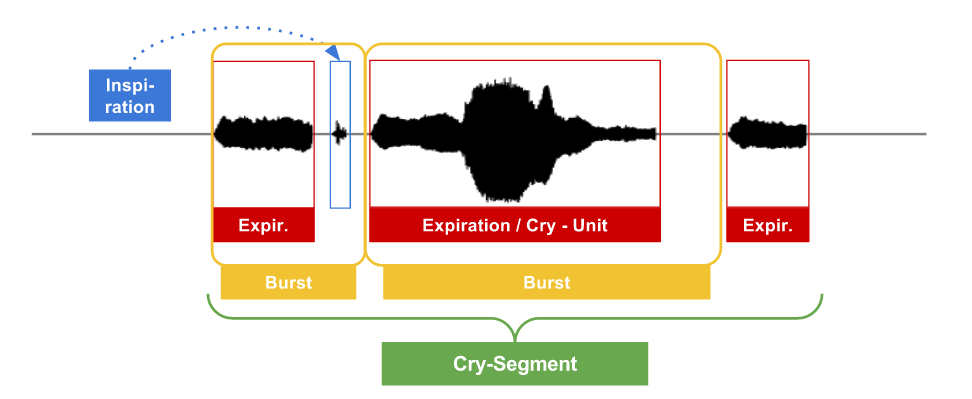
\includegraphics[width=0.9\textwidth]{bilder/cryVoc02.png}
	\caption{Veranschaulichung des Grundvokabulars für das Weinen}
	\label{img:cryVocabulary}
\end{figure}

Schreieinheiten werden von H. Golub und M. Corwin in eine der drei folgenden Kategorien eingeordnet, bezeichnet als \emph{Cry-Types} oder \emph{Cry-Modes}:

\begin{itemize}
	\item \textbf{Phonation} beschreibt eine Schreieinheit mit \glqq voller Vibration der Stimmbänder\grqq{} und einer Grundfrequenz zwischen 250 und \SI{700}{\hertz}. Entspricht umgangssprachlich einem Weinen mit einem \glqq klaren, hörbaren Ton\grqq{}.
	\item \textbf{Hyper-Phonation} beschreibt eine Schreieinheit mit einer \glqq falsetto-artigen Vibration der Stimmbänder\grqq{} und einer Grundfrequenz zwischen 1000 und \SI{2000}{\hertz}. Entspricht umgangssprachlich einem Weinen mit einem \glqq sehr hohen, aber klar hörbaren Ton\grqq{}.
	\item \textbf{Dysphonation} beschreibt eine Cry-Unit ohne klar feststellbare Tonhöhe, produziert durch Turbulenzen an den Stimmbändern. Entspricht umgangssprachlich dem \glqq Brüllen oder Krächzen\grqq{}.\cite[S. 61 - 62]{cryModel}
\end{itemize}

Die folgenden Eigenschaften können für einzelne Schreieinheiten festgestellt werden:

\begin{itemize}
	\item \textbf{Duration:} Die zeitliche Dauer der Schreieinheit.
	\item \textbf{Duration of Inspiration: }Die zeitliche Dauer der Pause zwischen zwei Schreieinheiten.
	\item \textbf{Grundfrequenz:} Die Grundfrequenz der Stimme wurde erläutert in \autoref{sec:theVoice}. Für eine Schreieinheit kann die durchschnittliche, die höchste und die niedrigste Grundfrequenz sowie die Varianz festgestellt werden.
	\item \textbf{Frequenz der Formanten:} Wie bei der Grundfrequenz kann der Durchschnitt, das Maximum, Minimum usw. für eine Schreieinheit berechnet werden.
	\item \textbf{Ratio2: } Verhältnis zwischen den Energien der Frequenzen unterhalb von \SI{2000}{\hertz} zu den Frequenzen oberhalb von \SI{2000}{\hertz}.
	\item \textbf{Cry-Mode Changes:} Häufigkeit des Wechsels des Cry-Modes innerhalb einer Schreieinheit.
	\item \textbf{Amplitude:} Die Lautstärke der Schreieinheit, gemessen in Dezibel.\cite[S. 85]{parentalPerception} \cite[S. 156]{threeCryTypes}
\end{itemize}

H. Golub und M. Corwin stellten weiterhin eine Reihe von Eigenschaften vor, die das zeitliche Verhalten der Grundfrequenz und der harmonischen Obertöne innerhalb einer Schreieinheit beschreiben.\cite[S. 73]{cryModel} Einige dieser Eigenschaften werden in \autoref{img:cryMelodies} in einem schematischen Spektogramm visualisiert.
\begin{itemize}
	\item \textbf{Pitch of Shift:} Grundfrequenz nach einem schnellen Anstieg zu Beginn der Schreieinheit.
	\item \textbf{Glide:} Kurzes, starkes ansteigen der Grundfrequenz.
	\item  \textbf{Glottal Roll:} Dysphonation, die häufig am Ende einer Schreieinheit nach einem Abfall der Grundfrequenz auftritt.
	\item  \textbf{Vibrato:} Mehr als vier starke Schwankungen der Grundfrequenz innerhalb einer Schreieinheit.
	\item  \textbf{Melody-Type } einer Schreieinheit. Meist: fallend, steigend/fallend, steigend, fallend/steigend, flach. 
	\item  \textbf{Continuity:} Verhältnis zwischen stimmhaften und nicht-stimmhaften Bereichen der Cry-Unit.
	\item  \textbf{Double Harmonic Break:} Das Aufkommen einer zweiten Serie von harmonischen Obertönen zwischen den eigentlichen harmonischen Obertönen einer Schreieinheit.
	\item  \textbf{Biphonation:} Das Aufkommen einer zweiten Grundfrequenz mit eigenen harmonischen Obertönen zusätzlich zu der eigentlichen Grundfrequenz.
	\item  \textbf{Noise Concentration:} Starke Energiespitzen zwischen 2000 und \SI{2300}{\hertz}.
	\item  \textbf{Furcation:} Plötzliches Aufteilen der Grundfrequenz und harmonischen Obertöne in mehrere, schwächere Obertöne.
\end{itemize}

\begin{figure}[h]
	\centering
	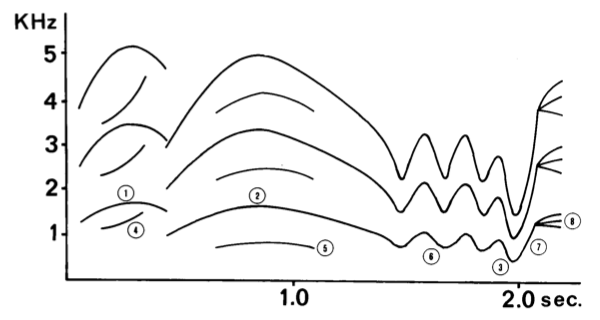
\includegraphics[width=0.7\textwidth]{bilder/melodyTypes.png}
	\caption[Schematisches Spektogramm eines beispielhaften Weinens]{Schematisches Spektogramm eines beispielhaften Weinens zur Visualisierung einiger Eigenschaften. Die schwarzen Linien zeigen  den Verlauf der Grundfrequenz und der Formanten. Die folgenden Eigenschaften werden gezeigt: (1) Pitch of Shift (2) Maximale Grundfrequenz (3) Minimum der Grundfrequenz (4) Biphonation (5) Double Harmonic Break (6) Vibrato (7) Glide (8) Furcation \cite[S. 142]{signal}}
	\label{img:cryMelodies}
\end{figure}

Die folgenden Eigenschaften werden in Bezug auf das gesamte Schrei-Segment, oder zumindest für eine Menge aufeinander folgender Schreieinheiten berechnet:

\begin{itemize}
	\item \textbf{Cry Latence: } Zeit zwischen Stimulus, wie zum Beispiel einem Nadelstich, und der ersten Schreieinheit.
	\item \textbf{Utterances: } Anzahl der Schreieinheiten im Segment.
	\item \textbf{Short Utterances: } Anzahl stimmloser Schreieinheiten im Segment.
	\item ... sowie statistische Auswertungen bezüglich aller in Eigenschaften, die für die Schreieinheiten eines Segmentes definiert wurden, wie beispielsweise der Durchschnitt aller Tonhöhen, Anzahl des Vorkommens bestimmter Melodiekonturen, Varianz der Länge der Schreieinheiten usw.\cite[S. 85]{parentalPerception}
\end{itemize}

Einige Krankheiten wurden in Zusammenhang mit dem vermehrten Vorkommen bestimmter akustischer Eigenschaften des Weinens gebracht. So wurde beispielsweise eine Korrelation zwischen dem Anstieg der durchschnittlichen Grundfrequenz, häufiger Biphonation und geringer Duration und dem Vorhandensein von Gehirnschäden beobachtet. Tendenziell niedrige Grundfrequenzen können auf Trisomie 13, 18 und 21 hinweisen.\cite[S. 85]{parentalPerception}

Ein Problem der Schreiforschung ist, dass sie bis heute weitestgehend unstandartisiert geblieben ist: \cite[S. 142]{signal}
\begin{itemize}
	\item Es gibt keine Liste, welche einen kompletten Überblick über alle (sinnvollen) akustischen Eigenschaften für Schreieinheiten oder Schrei-Segmente gibt. Viele Veröffentlichungen beziehen sich auf die Eigenschaften, die von H. Golub und M. Corwin vorgestellt wurden, und erweitern diese Liste durch eigene Vorschläge. 
	\item Es gibt keine Einigung darüber, welche der Eigenschaften die wichtigsten sind. Beispielsweise haben sich H. Golub und M. Corwin \cite{cryModel} vermehrt auf die Erkennung von Mustern im Melodieverlauf konzentriert, Zeskind et al. \cite{rythmic} haben vermehrt zeitliche Eigenschaften analysiert. Die Eigenschaft, die am häufigsten mit Schmerz, Krankheiten und sonstigen Abnormalitäten in Verbindung gebracht wurde, ist eine abnormal hohe oder niedrige Tonhöhe. Einige Eigenschaften, die von H. Golub und M. Corwin festgestellt wurden, ist nicht einmal gesichert, ob es sich nicht doch um technische Artefakte der damals verwendeten Analogtechnik handelt.\cite[S. 84 - 85]{parentalPerception}
	\item Selbst, wenn in verschiedenen Studien die selben Eigenschaften für das Weinen berechnet wurden, wie zum Beispiel die durchschnittliche Tonhöhe, ist nicht standardisiert, wie dieses zu berechnen ist. Mit \glqq durchschnittliche Tonhöhe des Weinens\grqq{} kann gemeint sein: 1.) die durchschnittliche Tonhöhe, errechnet aus den durchschnittlichen Tonhöhen aller Schreieinheiten. 2.) Die durchschnittliche Tonhöhe aller festgestellten Tonhöhen. 3.) Die durchschnittliche Tonhöhe nur von Ausatmungslauten usw.
	\item Zusammenhänge, die zwischen bestimmten Eigenschaften des Weinens und bestimmten Krankheitsbildern festgestellt wurden, haben häufig eine hohe Spezifität, aber niedrige Sensitivität. So wurde zum Beispiel festgestellt, dass Kinder, die am plötzlichen Kindstot sterben, fast immer eine Erhöhung der Frequenz des ersten Formanten in Verbindung mit häufigen Cry-Mode-Changes zeigen. Viele Babys, die nicht am plötzlichen Kindstot sterben, zeigen jedoch die selben Merkmale.\cite[S. 85]{parentalPerception}
\end{itemize}

\section{Automatisierte Klassifizierung und Bewertung}
\label{sec:learning}

Klassifizierung und Regression sind Teilgebiete des Wissenschaftsgebietes des \emph{Überwachten Lernens}, einem Teilgebiet des \emph{maschinellen Lernens}. Das Ziel beim Überwachten Lernen ist es, ein \emph{Modell}, auch bezeichnet als \emph{Hypothese}, zu entwerfen, welches aus den Eigenschaften einer \emph{Instanz} deren \emph{Kategorie} (auch \emph{Klasse}) oder \emph{Wert} bestimmt. Das Modell wird durch das Generalisieren einer Menge von Beispielen, für die die Klassen oder der Wert bereits bekannt sind, erstellt. Das Modell kann daraufhin eingesetzt werden, um für neue, bisher unbekannte Instanzen die jeweilige Kategorie oder Wert zu prognostizieren.\cite[S. 6 - 7]{machine_marsland}

Diese Begriffe werden anhand eines Beispiels erläutert. Das Ziel ist, für eine Instanz, einem \emph{Baby}, eine Klasse zu prognostizieren, wie zum Beispiel das Geschlecht. Ein Beispiel für einen zu prognostizierenden Wert ist \emph{der Grad des Schmerzes}. Die Prognose wird anhand von zwei Eigenschaften des Babys vorgenommen, und zwar 1.) die durchschnittliche Tonhöhe beim Weinen und 2.) die Augenfarbe. Zur Erstellung des Modells wird eine Datenbank zur Verfügung gestellt, in der für jedes Baby sowohl die Eigenschaften als auch das Geschlecht oder der Schmerzgrad protokolliert wurden.

%Den Feature-kram mit den bezeichnungen nochmal überprüfen!
Die Begriffe werden im folgenden mathematisch konkretisiert: Eine Instanz $x$ ist ein Vektor $x = ( f_1 \in F_1 ,\ \ldots\ , f_n \in F_n )$. $F_i$ wird als \emph{Eigenschaft}, \emph{Feature} oder \emph{Attribut} bezeichnet. In Bezug auf das eben genannte Beispiel ist $F_1 = $ \emph{durschnittliche Tonhöhe} und $F_2 = $ \emph{Augenfarbe}. Ein Beispiel für eine Instanz ist $x = ( \SI{300}{\hertz},$ \emph{blau}). Die Augenfarbe ist ein Beispiel für ein Feature mit einem diskreten Wertebereich, die Tonhöhe ein Beispiel für ein Feature mit einem kontinuierlichen Wertebereich. Die Menge aller möglichen Kombination der Features $F_1 \times , \ldots , \times F_n$ wird als \emph{Feature-Raum} bezeichnet. Der Trainingsdatensatz $D_{trainig}$ besteht aus einer Liste an Instanzen, wobei für jede Instanz die jeweilige Kategorie oder der Wert, gemeinsam Bezeichnet als \emph{Output} oder \emph{Target} $y \in Y$, bekannt ist. Ein Tupel aus einer Instanz und einem Output wird als \emph{Exempel} (engl. \emph{Example}) $e =(x,y)$ bezeichnet. $Y$ bezeichnet die Menge aller möglichen Outputs des Problems. Das heißt, $D_{training} = \big( \; (x_1, y_1), \ldots , (x_N, y_N) \; \big)$. Die Hypothese $H: X \mapsto Y$ ist eine Funktion, die von einer Instanz auf einen Output abbildet. Die Fehlerfunktion $E$ berechnet, wie häufig sich die Hypothese bei der Bestimmung der Targets eines Testdatensatzes $D_{test}$ irrt. Der Test- und der Trainingsdatensatz können die selben Instanzen, teilweise die selben oder gar keine gemeinsamen Instanzen beinhalten.\cite[S. 6 - 7, 18 - 19]{machine_marsland} \cite[S. 8 - 9]{learning_cart_dobra} 

%Nochmal mit den quellen checken!!
Bei der \textbf{Klassifizierung} wird eine Target als \emph{Klasse} bezeichnet. Die Menge aller möglichen Klassen eines bestimmten Problems $Y = \{ y_1 , \ldots, y_n\}$ ist nominal. Das heißt, dass die Menge diskret ist und die Targets einen \emph{qualitativen} Charakter haben. Ein Beispiel für ein Klassifizierungsproblem ist somit die Prognose des Geschlechtes für eine Instanz, also $Y = \{m, w\}$. Die Hypothese wird in diesem Fall als \emph{Klassifikator} $C$ bezeichnet.

Bei der \textbf{Regression} ist die Menge der möglichen Targets eines bestimmten Problems \emph{kontinuierlich} und hat einen \emph{quantitativen} Charakter, womit eine interne Ordnung der Outputs bestimmbar ist. Ein Beispiel für ein Regressions-Problem ist die Prognose des Körpergewichts des Babys mit $Y = \{ \SI{0}{\kilo\gram} , \ldots , \SI{10}{\kilo\gram} \}$. Die Hypothese wird in diesem Fall auch als \emph{Regressor} $R$ bezeichnet.\cite[S. 24]{learning_cart_dobra} \cite[S. 8]{machine_marsland} \cite[S. 28]{statistical_learning}

Handelt es sich bei den Targets um eine Ordinalskala, spricht man von \textbf{Ordinaler Klassifizierung} oder \textbf{Ordinaler Regression}, da die Ansätze zum Lösen solcher Probleme auf den Methoden der Klassifizierung und der Regression aufbauen und miteinander kombinieren.\cite[S. 1]{ordinalClassification} Ein Beispiel für ein solches Problem ist die Prognose des Schmerzgrades, mit $Y = \{ 0 , \ldots, 7  \}$ bei der NIPS (siehe \autoref{tab:nips} auf Seite \pageref{tab:nips}).

Es gibt eine Vielzahl an Algorithmen zum Finden des Klassifikators oder Regressors. Welcher Algorithmus der \glqq beste\grqq{} ist, also für einen Testdatensatz eine möglichst hohe \emph{Genauigkeit} oder einen möglichst geringen \emph{Klassifikationsfehler} erzeugt, ist abhängig von der konkreten Problemstellung. Auf die Bestimmung der Genauigkeit wird in \autoref{sec:howGoodIsMyClassifier} eingegangen. Ein Algorithmus, der in dieser Arbeit zur Erkennung der Stimmaktivität in \autoref{sec:vad} eingesetzt wird, ist der \emph{C4.5}-Algorithmus, welcher im folgenden Unterabschnitt erläutert wird.

\subsection{Klassifizierung mit den Algorithmen ID3 und C4.5}
\label{sec:id3}

Der ID3-Algorithmus zählt zu den sogenannten Entscheidungsbäumen, da der durch den Algorithmus entworfene Klassifikator die Form eines Entscheidungsbaumes annimmt. Die Vorraussetzung zur Verwendung des ID-3-Algorithmus ist, dass alle Attribute einen diskreten Wertebereich haben.\cite[S. 54]{machine_mitchell}. \autoref{tab:id3_example} zeigt einen Beispieldatensatz zur Erläuterung des Algorithmus. Die Instanzen sind \emph{Babys}, die Attribute sind $F_1 = $ \emph{Häufigkeit des Weinens} = \{ \emph{oft, normal, selten} \} und $F_2 = $ \emph{Lautstärke des Weinens} = \{ \emph{leise, laut} \}. Die Klasse $Y = $ \{ Ja, Nein \} gibt Auskunft darüber, ob das Baby an chronischen Schmerzen leidet. 

\begin{table}[h]
	\centering
	\caption{Beispieldatensatz für die Kassifizierung mit ID3}
	\label{tab:id3_example}
	\begin{tabular}{cccc}
		\toprule
		$x_i$    & $f_1 \in $ Häufigkeit   & $f_2 \in $ Lautstärke & $y_i \in $ Schmerz \\\midrule
		$x_1$  & oft                & laut          & Ja           \\
		$x_2$  & selten                & laut          & Ja           \\
		$x_3$  & normal                & leise          & Nein         \\
		$x_4$  & selten                & leise          & Nein           \\
		$x_5$  & normal                & laut         & Ja       \\
		$x_6$  & oft                & leise          & Ja       \\ \bottomrule  
	\end{tabular}
\end{table}

\autoref{img:id3tree} zeigt den Klassifikator, den der ID-3 Algorithmus für diesen Datensatz erzeugt. Es handelt sich um einen Entscheidungsbaum. In Jedem Knoten steht ein Attribut, welches einen Ast für jeden möglichen Attributwert bildet. In jedem Blatt steht eine Klasse.\cite[S. 134]{machine_marsland}

\begin{figure}[h]
	\centering
	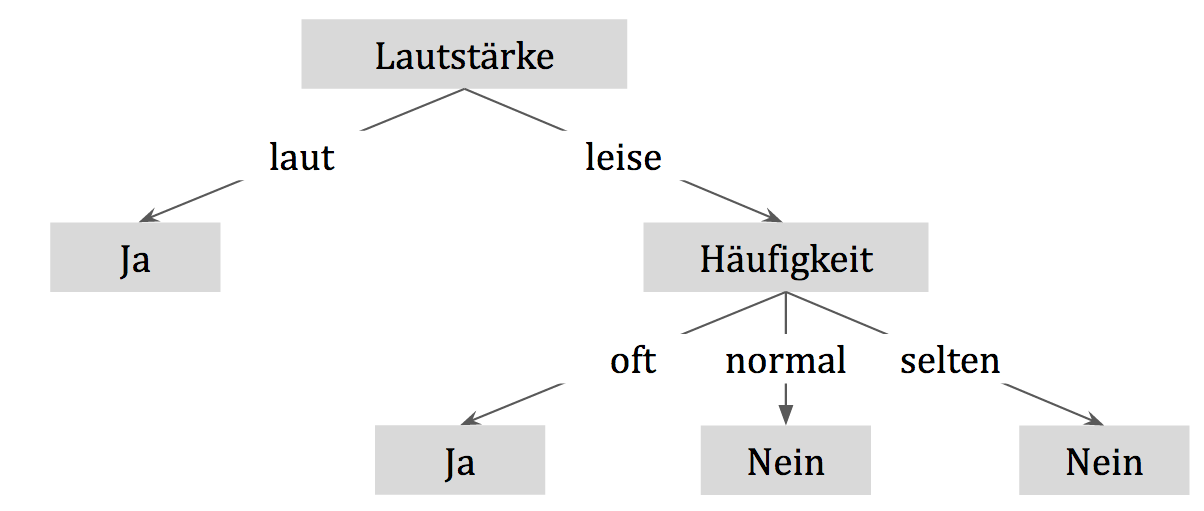
\includegraphics[width=0.6\textwidth]{bilder/id3tree02.png}
	\caption[Beispiel für einen Entscheidungsbaum zur Klassifizierung]{Entscheidungsbaum, der durch den ID3-Algorithmus für den Datensatz aus \autoref{tab:id3_example} erzeugt wird.}
	\label{img:id3tree}
\end{figure}

Der Entscheidungsbaum lässt sich in eine Reihe von \texttt{wenn ... dann ...} -Regeln transformieren. Jeder Weg von der Wurzel bis zu einem Blatt ergibt eine Entscheidungsregel, bei der die Attributwerte der entsprechenden Kanten konjunktiv verknüpft werden und die Klasse implizieren.\cite[S. 134]{machine_marsland} Die Entscheidungsregeln für den Baum aus \autoref{img:id3tree} sind:
\begin{itemize}
	\item \texttt{wenn}  \emph{Lautstärke = laut} \texttt{dann} \emph{Schmerz = Ja}
	\item \texttt{wenn}  \emph{Lautstärke = leise} \texttt{and} \emph{Häufigkeit = oft} \texttt{dann} \emph{Schmerz = Ja}
	\item \ldots
\end{itemize}

Der Entscheidungsbaum wird beim ID3 Algorithmus nach folgendem Muster erstellt: Die Konstruktion wird Top-Down vollzogen, das heißt beginnend bei der Wurzel bis zu den Blättern. In jedem Knoten wird ein Attribut in alle jeweils möglichen Werte aufgespalten. Um an der Wurzel zu entscheiden, welches Attribut zuerst aufgespalten wird, wird jedes Attribut einem statistischen Test unterzogen, um festzustellen, wie \glqq gut\grqq{} es zur Klassifizierung der Trainingsdaten beiträgt. Das \glqq beste\grqq{} Attribut wird ausgewählt und als Wurzel festgelegt. Nun wird ein Ast für jeden möglichen Wert des Attributs gebildet. Der Datensatz des Elternknotens wird in disjunkte Teilmengen aufgeteilt, wobei jedes Kind die Untermenge mit denjenigen Exempeln erhält, die den jeweiligen Attributwert besitzen. Daraufhin beginnt für jedes Kind der Prozess des Auswählens des \glqq besten\grqq{} Attributes von neuem. Ein Kind wird dann zu einem Blatt, wenn seine jeweilige Teilmenge nur noch aus Instanzen einer Klasse besteht und somit kein weiteres Aufteilen notwendig ist.\cite[S. 55]{machine_mitchell}

Zur Quantifizierung der Information wird die Entropie nach \autoref{eq:entropy} als Hilfsmittel definiert. $p_i$ ist die Wahrscheinlichkeit, dass in einem Datensatz $D$ ein Exempel mit der Klasse $i \in Y$ angetroffen wird. Die Entropie quantifiziert die \emph{Unreinheit des Datensatzes}. Ein Datensatz, dessen Exempel alle der selben Klasse angehören, hat die Entropie $0$. Ist die \emph{Unreinheit des Datensatzes} hingegen maximal, das heißt, dass der Datensatz exakt gleich viele Exempel jeder Klasse beinhaltet, ist die Entropie $1$. \cite[S. 135]{machine_marsland}

\begin{equation}
H(p) = -\sum_{i \in Y} p_i \cdot \log_{2} p_i
\label{eq:entropy}
\end{equation}

Es ist das Attribut in einem Knoten zu wählen, welches den höchsten \emph{Informatoinsgewinn} gewährleistet, das heißt, zu einer höchst möglichen \emph{Reinheit} in den Kindsknoten bei der alleinigen Unterteilung des Datensatzes auf Basis dieses Attributs führt. Der Informationsgewinn eines Features $F$ für den Datensatz $D$ wird nach \autoref{eq:informationGain} definiert. $|D|$ ist die Anzahl an Exempeln im Datensatz. $D_f$ ist die Untermenge mit den Exempeln, die für das Feature $F$ den Wert $f$ besitzen.\cite[S. 136 - 137]{machine_marsland}

\begin{equation}
\text{Gain}(D,F) = H(D) - \sum_{f \in F} \frac{|D_f|}{|D|} H(D_f)
\label{eq:informationGain}
\end{equation}

Die Erstellung eines Entscheidungsbaumes mit Hilfe des ID3-Algorithmus wird folgendermaßen als Pseudocode definiert. Der Input des Algorithmus ist der Datensatz $D$ und der Feature-Raum $F_{all}$, der Output ist der Entscheidungsbaum.\cite[S. 139]{machine_marsland}
%% Think about untere Linie entfernen!
\vspace{3mm}

\footnotesize

\noindent\textbf{ID3}($D,F_{all}$) \noindent\rule{0.85\linewidth}{0.3pt} \\[-3mm]
\begin{itemize}
\item \textbf{Wenn} alle Examples $e \in D$ das selbe Label haben:
	\begin{itemize}
	\item \textbf{return} eine Blatt mit diesem Label
	\end{itemize}
\item \textbf{Sonst}
	\begin{itemize} 
	\item \textbf{Wenn} keine Attribute übrig sind zum Testen
		\begin{itemize}
		\item \textbf{return} ein Blatt mit dem häufigsten Label in dem Datensatz
		\end{itemize}
	\item \textbf{Sonst:} 
		\begin{itemize}
		\item Wähle das Feature $\hat{F}$ als den nächsten Knoten, dass den Informationsgewinn für den Datensatz $D$ nach \autoref{eq:informationGain} maximiert.
		\item Füge einen Ast für jeden möglichen Wert $f \in \hat{F}$ von dem Knoten hinzu.
		\item Für jeden Ast:
			\begin{itemize}
			\item Berechne $D_f$, in dem $\hat{F}$ von der Liste der Features entfernt wird.
			\item Rufe \textbf{ID3}($D_f, F_{all} / \hat{F}$) rekursiv auf.
			\end{itemize}
		\end{itemize}
	\end{itemize} 
\end{itemize}

%\noindent\rule{\linewidth}{0.3pt}

%\vspace{3mm}

\normalsize

Der ID3-Algorithmus hat folgende \textbf{Nachteile}:
\begin{itemize}
\item Der Algorithmus akzeptiert keine kontinuierlichen Features.\cite[S. 72]{machine_mitchell}
\item Der Algorithmus neigt zu \emph{Overfitting}. Overfitting bedeutet, dass der Klassfikator $C$ zwar einen möglichst geringen Klassifikationsfehler in Bezug auf den gegebenen Trainingsdatensatz erzeugt, es jedoch einen anderen Klassifikator $C'$ gibt, welcher für diesen speziellen Trainingsdatensatz schlechter performt, jedoch einen geringeren Fehler als $C$ in Bezug auf \emph{alle möglichen Instanzen dieses Problems} erzeugt. Umgangssprachlich formuliert bedeutet Overfitting, dass der Klassifikator den Trainingsdatensatz \glqq auswendig gelernt hat\grqq{} und nicht genügend generalisiert, um auf im Training nicht enthaltene Instanzen angewendet werden zu können. Overfitting im Zusammenhang mit dem ID-3 Algorithmus wird durch \emph{Rauschen im Trainingsdatensatz} bedingt.
\item Der Algorithmus bevorzugt greedy Attribute, die zum Zeitpunkt der Berechnung den höchsten Informationsgewinn gewährleisten. Dabei besteht die Gefahr, dass der Algorithmus in ein lokales Maximum läuft.\cite[S. 66 - 70]{machine_mitchell}
\end{itemize}

Der \emph{C4.5}-Algorithmus erweitert den \emph{ID3}, um dessen Nachteile zu kompensieren. Er ermöglicht die Verwendung kontinuierlicher Attribute und bietet Lösungsansätze zur Verminderung von Overfitting.

Für einen Knoten mit einem kontinuierlichen Attribut werden beim \emph{C4.5}-Algorithmus genau zwei Äste gebildet. Es wird ein Grenzwert für das Feature festgelegt, bei dessen Unterschreitung der linke, und bei dessen Überschreitung der rechte Ast gewählt wird (oder, je nach Implementierung, umgedreht). Das Vorgehen zum Finden eines solchen Grenzwertes ist wie folgt:

\begin{enumerate}
\item Ordne alle Exemple nach ihrem jeweiligen Wert des kontinuierlichen Attributs $F_c$, für das der Grenzwert gesucht wird. 
\item Identifiziere benachbarter Exemple mit unterschiedlichen Klassen. Die Attributwerte dieser Exemple sind mögliche Kandidaten für einen Grenzwert.
\item Berechne den Informationsgewinn bei Setzung des Grenzwertes auf jeden gefundenen Kandidaten. 
\item Wähle denjenigen Grenzwert, der den höchsten Informationsgewinn gewährleistet.\cite[S. 73]{machine_mitchell}
\end{enumerate}

\autoref{img:continuos_variable} visualisiert einen Knoten mit einem kontinuierlichen Attribut $F_c$, der durch einen Grenzwert in zwei Äste aufgespalten wird.


\begin{figure}[h]
	\centering
	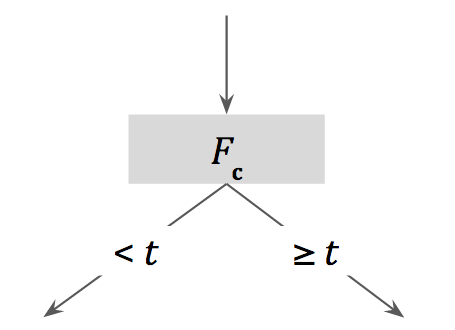
\includegraphics[width=0.35\textwidth]{bilder/continuos_variable.png}
	\caption{Aufspaltung eines kontinuierlichen Attributs im Entscheidungsbaum}
	\label{img:continuos_variable}
\end{figure}

Das als Overfitting beschriebene Problem lässt sich vermeiden, in dem die Tiefe des Entscheidungsbaumes reduziert wird. Diese Begrenzung wird als \emph{Beschneiden} oder \emph{Pruning} bezeichnet. Es gibt grundlegend zwei verschiedene Ansätze:


\begin{description}
 \item[Pre-Pruning:] Ab der Überschreitung einer bestimmten Tiefe wird der Algorithmus frühzeitig gestoppt und ein Knoten, welcher die maximale Tiefe überschreitet, zwangsweise zu einem Blatt umgewandelt. 
 \item[Post-Pruning:] Zuerst wird der komplette Entscheidungsbaum aufgebaut und Overfitting zugelassen. Im Nachhinein wird der Entscheidungsbaum in seiner Tiefe reduziert. Eines der am weitest verbreiteten Post-Pruning-Algorithmen ist das \emph{Reduced Error Pruning}. Dabei wird ein Knoten des Entscheidungsbaumes zu einem Blatt umgewandelt und dem Blatt das Label zugewiesen, welches in seinem Sub-Baum am häufigsten vorkommt. Daraufhin wird der originale Entscheidungsbaum sowie der beschnittene Entscheidungsbaum verwendet, um den Testdatensatz zu klassifizieren. Ist der Klassifizierungsfehler des beschnittenen Baumes nicht höher als der des originalen Baumes, wird das Pruning übernommen. Dieses Vorgehen wird für jeden Knoten des Entscheidungsbaumes angewandt. \cite[S. 68 - 70]{machine_mitchell} 
\end{description}


\subsection{Gütemaße binärer Klassifikatoren}
\label{sec:howGoodIsMyClassifier}

eine binäre Klassifikation ist eine, bei der es genau zwei Klassen gibt, das heißt $|Y| = 2$. Applikationsabhängig werden die beiden Klassen beispielsweise als \emph{Positive} und \emph{Negative}, $1$ und $0$ oder \emph{True} und \emph{False} bezeichnet. Wird bei einer Klassifizierung ein tatsächliches Positive korrekt als Positive prognostiziert, spricht man von einem \emph{True Positive} [TP]. Wird hingegen ein tatsächliches Positive fälschlicherweise als Negative prognostiziert, spricht man von einem \emph{False Negative} [FN]. Bei der Klassifizierung von Negatives spricht man dementsprechend von \emph{True Negatives} [TN] und \emph{False Positives} [FP]. Die \emph{Confusion Matrix} in \autoref{img:Confusion-Matrix} gibt eine Übersicht über die vier möglichen Klassifizierungsergebnisse. \cite[S. 213 - 214]{machine_kubat}

\begin{figure}[h]
	\centering
	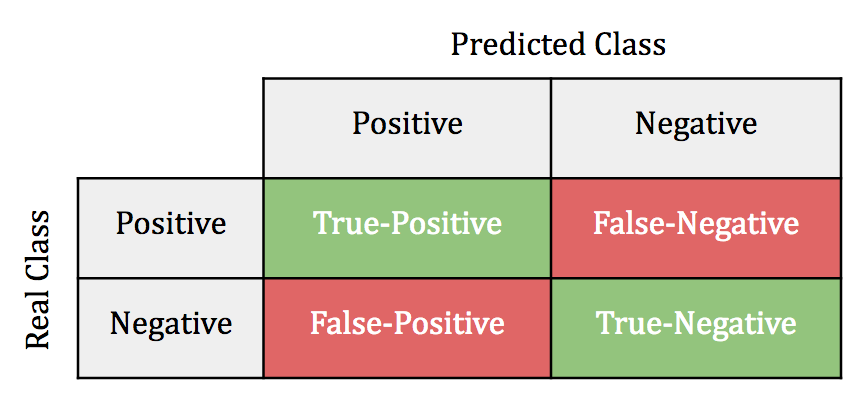
\includegraphics[width=0.6\textwidth]{bilder/Confusion-Matrix02.png}
	\caption[Confusion Matrix]{Confusion Matrix (nach: \cite[S. 214]{machine_kubat})}
	\label{img:Confusion-Matrix}
\end{figure}

Die insgesamte Güte einer Klassifizierung wird durch die \emph{Genauigkeit} (engl. \emph{Accuracy}) nach \autoref{eq:accuracy} bestimmt. Eine Genauigkeit von 100\% bedeutet, dass \emph{alle} Instanzen richtig klassifiziert wurden, eine Genauigkeit von 50\% bedeutet, dass die Hälfte aller Instanzen richtig klassifiziert wurden. Je höher die Genauigkeit, desto geringer der Klassifikationsfehler. \cite[S. 214]{machine_kubat}

\begin{equation}
\text{Accuracy} = \frac{TP+TN}{TP+TN+FN+FP}
\label{eq:accuracy}
\end{equation}

Mit Hilfe der Genauigkeit wird die insgesamte Performance des Klassifikators gemessen. Der Wert allein gibt jedoch keinen Aufschluss darüber, ob der Klassifikator eher eine Tendenz zur falschen Klassifizierung von Positives oder Negatives hat. Bei einer Datenbank mit der selben Anzahl an Positives und Negatives kann eine Genauigkeit von 50\% beispielsweise dadurch entstehen, dass \emph{alle} Instanzen als Positives markiert werden. Das heißt, dass alle Positives richtigerweise als Positives, aber alle Negatives fälschlicherweise ebenfalls als Positives klassifiziert werden. Im umgedrehten Fall ergibt die Klassifizierung aller Instanzen als Negatives ebenfalls eine Genauigkeit von 50\%. In einem dritten Fall irrt sich die Klassifikator gleich oft bei der Einordnung der Negatives und Positives. 

Die Maße \emph{Sensitivität} (engl. \emph{Sensitivity}) und  \emph{Spezifität} (engl. \emph{Specificity}) geben Aufschluss über die Performance des Klassifikators bei der Prognose der Positives und Negatives. Die Sensitivität, auch bezeichnet als \emph{True-Positive-Rate}, bemisst den Anteil tatsächlicher Positives, die auch als solche erkannt wurden, nach \autoref{eq:sensitivity}. Eine Sensitivität von 100\% bedeutet, dass alle in der Datenbasis enthaltenen tatsächlichen Positives auch als solche erkannt  wurden. Die Erkennungsrate der Negatives hat keinen Einfluss auf die Sensitivität. Eine hohe Sensitivität lässt sich somit \glqq einfach\grqq{} erzielen, in dem man \emph{alle} Instanzen immer als Positives klassifiziert.\cite[S. 222]{machine_kubat}

\begin{equation}
\text{Sensitivity} = \frac{TP}{TP+FN}
\label{eq:sensitivity}
\end{equation}

Die Spezifität nach \autoref{eq:specificity} bestimmt analog zur Sensitivität den Anteil der Negatives, die als solche klassifiziert wurden. 

\begin{equation}
\text{Specificity} = \frac{TN}{TN+FP}
\label{eq:specificity}
\end{equation}

Ein Klassifikator, der alle Instanzen als Positives markiert, hat zwar eine Sensitivität von 100\%, aber eine Spezifität von 0\%. Ergeben zwei verschiedene Klassifikationsmodelle sehr ähnliche Genauigkeiten, hilft die Bestimmung der Sensitivität und der Spezifität bei der Auswahl des für den Anwendungsfall adäquateren Klassifikators. So ist beispielsweise bei der Bestimmung von schweren Krankheiten eventuell ein Klassifikator mit höherer Sensitivtät wünschenswert, um die Wahrscheinlichkeit zu minimieren, dass die entsprechende Krankheit nicht erkannt wird.\cite{sens-and_spec}  \cite[S. 222]{machine_kubat}


\chapter{Konzept zur automatisierten Schmerzbewertung anhand akustischer Signale}
\label{sec:concept}

%Ergänenzen!
In Kapitel \ref{sec:medicalFoundations} wurde vorgestellt, wie die Schmerzdiagnostik bei Neugeborenen im medizinischen Alltag mit Hilfe multimodaler Schmerz-Scales durchgeführt wird. Das Ziel ist nun der Entwurf eines Konzeptes für ein System, das die Schmerzdiagnostik nach diesem Vorbild auf Basis akustischer Signale automatisiert und kontinuierlich vornimmt. In diesem Kapitel wird ein Überblick über das entworfene Konzept gegeben. Dazu wird in Kapitel \ref{sec:system_literature} zunächst ein Überblick über Veröffentlichungen mit ähnlichen Zielstellungen gegeben.

\section{Literaturüberblick}
\label{sec:system_literature}

Ein großer Teil der Veröffentlichungen, die sich in das Feld der Analyse von Audioaufnahmen Neugeborener einordnen lassen, stellen Methoden zur Klassifizierung einzelner Schreieinheiten vor, entweder bezüglich der Weinursache (Hunger, Angst, Schmerz, ... ) oder zur Diagnose bestimmter Krankheiten. Diese Methoden sind in den meisten Fällen nicht für eine kontinuierliche Analyse vorgesehen, sondern haben das Ziel, die Eignung bestimmter Features oder Klassifizierungsalgorithmen für die jeweiligen Klassifizierung zu erforschen. Beispiele für solche Veröffentlichungen sind die von Abdulaziz et al. \cite{class_abdulaziz} oder Fuhr et al. \cite{comparisonOfLearning}.

Várallyay stellte in seiner Dissertation \glqq Analysis of the Infant Cry with Objective Methods\grqq{} \cite{cry_thesis} Methoden zur automatisierten Analyse kindlicher Lautäußerungen vor. Das primäre Ziel der Dissertation war die Erforschung der Unterschiede zwischen den Lautäußerungen gesunder und tauber Neugeborener. Die Algorithmen zur automatisierten Analyse der Audiosignale waren ein \glqq Nebenprodukt\grqq{} zur schnelleren Datenauswertung. Die Auswertung musste nicht kontinuierlich erfolgen. In der vorgestellten Verarbeitungs-Pipeline wurde das Eingangssignal in Zeitfenster weniger Millisekunden zerlegt und jedes Fenster nach Entscheidungsregeln als \emph{stimmhaft} oder \emph{nicht stimmhaft} markiert. Die stimmhaften Signalfenster wurden zu \emph{Segmenten} zusammengefasst (welche in Kapitel \ref{sec:acousticModel} als Schreieinheiten bezeichnet werden). Auf Basis der Segmente wurden Auswertungen bezüglich des Zeitbereiches (Durchschnittliche Segmentlänge, Pausenlängen etc.), des Frequenzbereiches (Grund-Frequenz, Formanten-Frequenzen etc.) und des Melodieverlaufes vorgenommen. Analysiert wurden Audioaufnahmen von Babys mit einer Länge von 10 bis \SI{100}{\second}. Auf Basis der Auswertungsergebnisse stellte Varallyay die wichtigsten Unterscheidungsmerkmale zwischen tauben und gesunden Babys fest. In der Dissertation \cite{cry_thesis} wird ein Überblick über das Vorgehen und die Ergebnisse gegeben. Die Verarbeitungsschritte wurden detaillierter in einzelnen Veröffentlichungen beschrieben, wobei der Autor dieser Arbeit nur den Zugriff auf einige dieser Veröffentlichungen erhalten konnte.

Cohen et al. haben 2012 in der Veröffentlichung \glqq Infant Cry Analysis and Detection\grqq{} \cite{cohenCry}  ein System zur Analyse der akustischen Signale von Neugeborenen vorgestellt. Dieses System klassifizierte die Audiosignale in eine der drei Klassen \emph{Cry, No Cry} und \emph{No Activity}. Die Klasse \emph{Cry} bezeichnet Lautäußerungen, die eine potentiell Gefahr für das Baby anzeigen, wie z.B. wie Schmerz oder Hunger. Die Klasse \emph{No Cry} bedeutete, dass das Baby zwar Laute von sich gibt, diese aber keine potentielle Gefahr anzeigen. Die Klasse \emph{No Activity} bezeichnete keinerlei Lautäußerung. Die Verarbeitungs-Pipeline wurde detailliert vorgestellt und ist für die kontinuierliche Verarbeitung mit einer gewissen Verzögerungszeit spezialisiert. Das Signal wird in überlappende \emph{Segmente} \`{a} \SI{10}{\second} zerlegt. Die Stimmaktivität in den Segmenten wird algorithmisch festgestellt. Wenn Aktivität vorliegt, wird das Segment in Sektionen \`{a} \SI{1}{\second} zerlegt und die Stimmaktivität für jede Sektion gemessen. Wird genügend Stimmaktivität in einer Sektion festgestellt, wird die Sektion in \emph{Frames} \`{a} \SI{32}{\milli\second} zerlegt und Attribute für jeden Frame errechnet. Mit Hilfe von Entscheidungsregeln werden die Frames in \emph{Cry, No-Cry} oder \emph{No Activity} klassifiziert, wobei kontextuelle Informationen der umliegenden Frames mit einbezogen werden. 

%Aus den Klassen der Frames wird auf die Klasse der Sektion geschlossen, und aus den Klassen der Sektionen auf die Klasse des Segmentes. Das System hat mit den Anforderungen dieser Arbeit gemeinsam, dass ebenfalls die kontinuierliche Verarbeitung im Vordergrund steht. Der Nachteil an dieser Methode ist, dass die zeitliche längste Einheit, für die die Klassifizierung vorgenommen wird, unflexibel auf \SI{10}{\second} festgelegt ist. Daher müsste diese Verarbeitungs-Pipeline abgewandelt werden, um anstelle der Ableitung der drei genannten Klassen einen Pain Score ableiten zu können, die einen längeren Beobachtungszeitraum als \SI{10}{\second} benötigt.

Pal et al.  haben 2006 in der Veröffentlichung \glqq Emotion detection from infant facial experessions and cries\grqq{} \cite{palEmotion} ein System vorgestellt, welches aus den akustischen Eigenschaften des Weinens die Emotion ableitet. Die zu erkennenden Emotionen waren \emph{Trauer, Wut, Hunger, Angst und Schmerz}. Es wurde nicht erwähnt, ob die Analyse kontinuierlich oder nicht kontinuierlich erfolgt. Bei der Verarbeitung der akustischen Signale werden die Attribute \emph{Grundtonhöhe} und die \emph{Frequenz der ersten drei Formanten} extrahiert und mit einem Klassifizierungsalgorithmus klassifiziert. Es wurde nicht beschrieben, inwiefern die Eigenschaften aus kurzen Signalfenstern oder längeren Signalabschnitten errechnet wurden, welche Vorverarbeitungsschritte angewandt wurden und ob die Klassifizierung auf Ebene der Signalfenster oder über längere Zeitabschnitte hinweg geschieht.

Zamzi et al.  haben 2016 in der Veröffentlichung \glqq An Approach for Automated Multimodal Analysis of Infants' Pain\grqq{} \cite{zamziMultimodal} ein System zur automatisierten und kontinuierlichen multimodalen Analyse von Neugeborenen zur Ableitung des Schmerzes vorgestellt. Das System trägt den Namen \emph{MPAS}. Der Schmerzgrad wird aus den Analyseergebnissen der monomodalen Schmerzindikatoren für \emph{Gesichtsausdruck, Körperbewegung, Vitalfunktionen und Weinen} errechnet. Das System kommt der Aufgabenstellung dieser Masterarbeit am nächsten, da es ebenfalls um die Ableitung von Schmerz in einem multimodalen Verbund geht. Der Schmerz wird hier \glqq direkt\grqq{} abgeleitet, ohne die Scoringsysteme der Schmerzscales zu verwenden. Während in der Veröffentlichung die Analyse der ersten drei genannten Schmerzindikatoren angekündigt wurde, wurden daraufhin die Methoden zur Analyse der akustischen Signale \emph{nicht} erläutert. Auch die ersten Validierungsergebnisse beziehen sich nur auf den Gesichtsausdruck, die Körperbewegung und die Vitalfunktionen. Es ist nicht klar, ob die Miteinbeziehung akustischer Signale fallen gelassen wurde. Die Ausführungen konzentrieren sich dazu vermehrt auf die Methoden zur Kombination der Auswertungsergebnisse der monomodalen Schmerzindikatoren.

H. Golub und M. Corwin erwähnen in \glqq A Physioacoustic Model of the Infant Cry\grqq{} \cite{cryModel} , bereits in den achtziger Jahren ein System zur computergestützten und voll automatisierten Analyse von Cry-Segmenten implementiert zu haben. Das System nimmt 1.) eine Audioaufnahme, gespeichert auf einer Kasette, an, 2.) berechnet Formanten, Grundfrequenz und Amplitude gegen die Zeit, 3.) samplt die Grundfrequenz-Kontur, 4.) berechnet insgesamt 88 akkumulierte Features für das gesamte Segment und 5.) zieht Schlussfolgerungen aus den 88 Eigenschaften, wie zum Beispiel die Diagnose einer bestimmten Krankheit.\cite[S. 75 - 76]{cryModel} Abseits der kurzen Erwähnung der Existenz dieses ersten automatisierten Analysesystems für das Weinen von Babys in \cite{cryModel} konnte der Autor dieser Arbeit keine Implementierungsdetails oder sonstige genauere Ausführungen über das System finden, welche für diese Arbeit von höchstem Interesse gewesen wären.


%\section{Anforderungen an das Konzept}
%\label{sec:Anforderungen}

%Ziel dieser Arbeit ist der Entwurf eines Systems zur automatisierten Feststellung und Visualisierung von Pain Scores beliebiger Pain Scales mit dem Fokus auf den Schmerzindikator \glqq Weinen\grqq. Das System muss folgenden Anforderungen erfüllen:

%\begin{enumerate}
%	\item Das System muss dazu in der Lage sein, aus den akustischen Eigenschaften des Weinens eines Babys den Schmerz Score bezüglich einer Pain Scale abzuleiten.
%	\item Das System muss dazu in der Lage sein, die abgeleiteten Schmerz Scores zu visualisieren.
%	\item Das System muss dazu in der Lage sein, beliebige Pain Scales einzubinden. 
%	\item Die System muss dazu in der Lage sein, die Analyse auch bei nicht-optimalen akustischen Bedingungen durchzuführen.
%	\item Das System muss dazu in der Lage sein, die Analyse kontinuierlich durchzuführen.
%\end{enumerate}

%Der \textbf{Input} des Systems ist folglich ein Audiosignal, welches kontinuierlich in das System gegeben wird. Der \textbf{Output} ist eine Visualisierung der abgeleiteten Pain Score, welche kontinuierlich erzeugt wird.

\section{Überblick über die Verarbeitungsschritte}
\label{sec:pipeline}

%In Kapitel \ref{sec:system_literature} wurden verschiedene Konzepte vorgestellt, deren Fokus ebenfalls die Analyse und Auswertung von Audioaufnahmen kindlicher Lautäußerungen waren und somit der Aufgabenstellung dieser Arbeit ähneln. Keines der präsentierten Konzepte eignet sich, um mit nur leichten Anpassungen übernommen werden zu können: Entweder wurden die Verarbeitungsschritte nicht für die kontinuierliche Verarbeitung konzipiert \cite{class_abdulaziz} \cite{comparisonOfLearning} \cite{cry_thesis}, nicht genügen abstrahiert, um für andere Klassifizierungen als die ursprünglich geplanten abgewandelt werden zu können \cite{cohenCry}, oder die Verarbeitungs-Pipeline wurde nicht vorgestellt. \cite{palEmotion} \cite{zamziMultimodal}.

Für diese Arbeit wurde die folgende Verarbeitungs-Pipeline entworfen. Sie wird in in Abbildung \ref{img:architecture-overview} schematisch visualisiert. 

%To Do: Kapitel hinzufügen.
\begin{enumerate}[leftmargin=*]
	\item \textbf{Input: } Ein Audiosignal, das möglicherweise Weinen eines Babys enthält. Es wird kontinuierlich in das System gegeben.
	
	\item \textbf{Erkennung Schreigeräuschen}. (engl. \emph{Detection of Cry-Sounds}) Zunächst muss festgestellt werden, ob und wo in dem Signal kindliche Lautäußerungen vorhanden sind. Ein Algorithmus zur Feststellung von Stimmaktivität, bezeichnet als Voice Activity Detection, analysiert das Signal und markiert stimmhafte Bereiche. Aus den stimmhaften Bereichen werden die Anfangs- und Endzeitpunkte der Schreieinheiten geschlussfolgert, welche die Basis aller darauf folgenden Verarbeitungsschritte bilden. Dieser Verarbeitungsschritt wird in Kapitel \ref{sec:vad} detaillliert erläutert.
	
	\item \textbf{Segmentierung} (engl \emph{Segmenting}). Es ist nicht sinnvoll, einen Schmerz-Score auf Basis nur einer einzelnen Schreieinheit ableiten zu wollen. Daher werden \emph{Schrei-Segmente} gebildet, in dem Schreieinheiten, die nahe beieinander liegen, zu Segmenten gruppiert werden. Diese Schrei-Segmente bilden die Grundlage für das Scorings des Weinens. 
		
	\item \textbf{Extrahierung von Eigenschaften und Prognose des Scores} (engl. \emph{Feature Extraction} und \emph{Prediction of Score}). Für jedes Segment werden Eigenschaften bezüglich der akustischen Informationen des Weinens berechnet, wie zum Beispiel die durchschnittliche Tonhöhe, die durchschnittliche Pausenlänge usw. Auf Basis dieser Eigenschaften wird ein Score für das Weinen des jeweilige Schrei-Segmentes berechnet. Dieser Score kann in einem multimodalen System verwendet werden, um in Verbindung der Scores der anderen Schmerzindikatoren den schlussendlichen Scherz-Score zu berechnen. Da die Segmentierung, die Extrahierung der Eigenschaften und das Ableiten der Scores eng zusammenhängen, werden sie in Kapitel \ref{sec:deduction} erläutert.
	
	\item \textbf{Output: Visualisierung} (engl. \emph{Visualisation}) Es wird für jeden Zeitpunkt des Eingangssignals der im vorhergehenden Verarbeitungsschritt prognostizierte Score visualisiert. Bei dem vorgestellten Visualisierungskonzept wird das Scoring farblich codiert und auf einer Zeitachse abgebildet. Die Visualisierung wird in Kapitel \ref{sec:visualisation} erläutert.	
	
	\end{enumerate}

\begin{figure}[h]
	\centering
	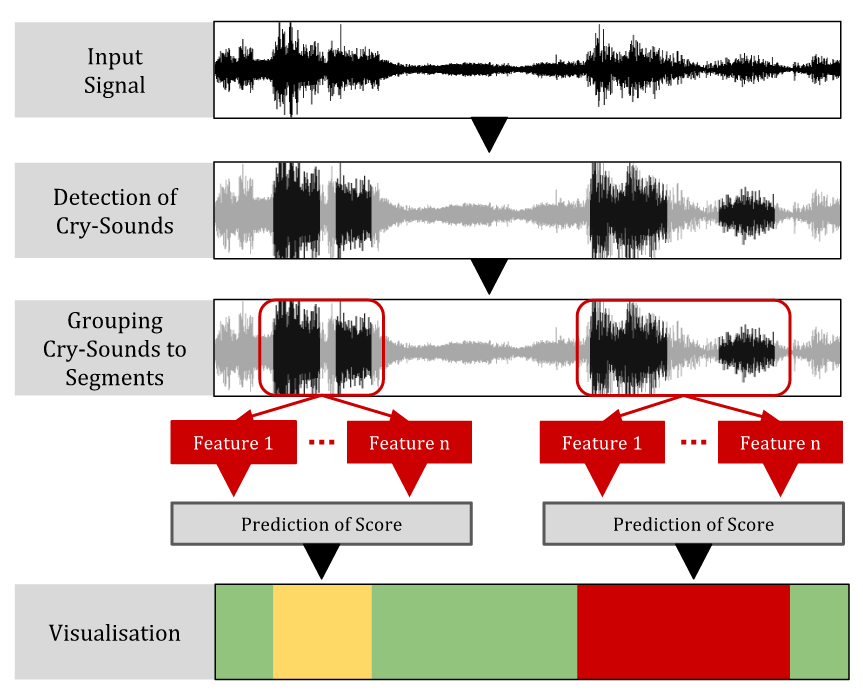
\includegraphics[width=0.75\textwidth]{bilder/konzept03.png}
	\caption{Überblick über die Verarbeitungs-Pipeline dieser Arbeit}
	\label{img:architecture-overview}
\end{figure}

Der erste Verarbeitungsschritt, die Erkennung der Schreigeräuschen, ist notwendig, damit für die Prognose des Scores für das Weinen auch nur solchen Informationen genutzt werden, die tatsächlich von einem Baby stammen, und nicht das Hintergrundrauschen. Würde man beispielsweise das Scoring für das Weinen hauptsächlich auf der Tonhöhe des Weinens ableiten und vorher nicht solche Geräusche verwerfen, die nicht von einem Baby stammen, würde diese mit in die Berechnung des Scores einfließen und das Ergebnis verfälschen. Diese Notwendigkeit wurde sowohl von Várallyay \cite{cry_thesis} als auch von Cohen et al. \cite{cohenCry} beschrieben. 


Der zweite Verarbeitungsschritt, die Segmentierung, ist notwendig, da wie in Kapitel \ref{sec:medicalFoundations} beschrieben der Schmerz-Score für einen längeren Beobachtungszeitraum bestimmt wird und in einem kontinuierlichen System sinnvolle Anfangs- und Endzeitpunkte für diese Beobachtungszeiträume gefunden werden müssen. Keine der in Kapitel \ref{sec:system_literature} vorgestellten Veröffentlichungen stellt ein Methode zur Gruppierung der Schreigeräusche vor, die für diese Arbeit übernommen werden könnte. Cohen et al. \cite{cohenCry} schlägt eine Feste Segmentlänge von 10 Sekunden vor. Es wurde sich gegen diesen Ansatz entschieden, da einige der in Kapitel \ref{sec:medicalFoundations} beschriebenen Pain-Scales längere Beobachtungszeiträume fordern. In der Promotion von Várallyay \cite{cry_thesis} war dieser Verarbeitungsschritt nicht notwendig, da die Analyse nicht kontinuierlich umgesetzt werden musste und die zu Analysierenden Segmente manuell geschnitten wurden. Pal et al. \cite{palEmotion} erwähnen keine Gruppierung von Schregeräuschen. Deshalb wurde in dieser Arbeit ein simpler Algorithmus zur Segmentierung entwickelt, welcher in Kapitel \ref{sec:segmenting} vorgestellt wird.

Die Berechnung von akustischen Eigenschaften des Weinens und der darauf folgenden Prongnose des Schmerz-Scores ist ein Verarbeitungschritt, der grundlegend in allen in Kapitel \ref{sec:system_literature} vorgestellten Veröffentlichungen angewendet wird. Je nach Ziel der Prognose werden unterschiedliche Eigenschaften und Klassifizierungs- oder Regressionsmethoden berechnet. 


\subsection{Automatisierte Visualisierung der Schmerzbewertung im multimodalen Verbund}



Dies würde der Visualisierung eines Schmerz-Score entsprechen, insofern es sich bei der verwendeten Schmerz-Scale allein um eine monomodale Scale handelt, die nur das Weinen in das Scoring mit einbezieht. In einem multimodalen System müssten vor der Visualisierung die Scores der anderen Schmerzindikatoren dem für das Weinen vergebenen Score aufaddiert werden. In diesem Fall wäre das Visualisierungskonzept ebenfalls anwendbar.
\chapter{Detektion von Schreigeräuschen in Audiosignalen}
\label{sec:vad}

Der erste notwendige Schritt zur Schmerzdiagnostik auf Basis eines Audiosignals ist festzustellen, ob in dem Signal überhaupt kindliche Lautäußerungen vorhanden sind. Das Ziel ist, in einem Audiosignal diejenigen Bereiche zu markieren, in denen Stimmaktivität vorhanden ist und daraufhin die Anfangs- und Endzeitpunkte  der Schreieinheiten zu bestimmen. \autoref{img:vad01} verdeutlicht diese Aufgabe an einem Beispiel: Der obere Graph zeigt in Schwarz ein Audiosignal. Die rote Linie, die das Signal überspannt, zeigt, welche Regionen Stimme enthalten, wobei $1 \: \hat{=} $ \emph{stimmhaft} (engl. \emph{voiced}) und $0 \: \hat{=}  $ \emph{nicht stimmhaft} (engl. \emph{not voiced}, in diesem Zusammenhang auch bezeichnet als \emph{Stille}). Im unteren Schema wurden die stimmhaften Signalbereiche zu Schreieinheiten zusammengefasst.

\begin{figure}[h]
	\centering
	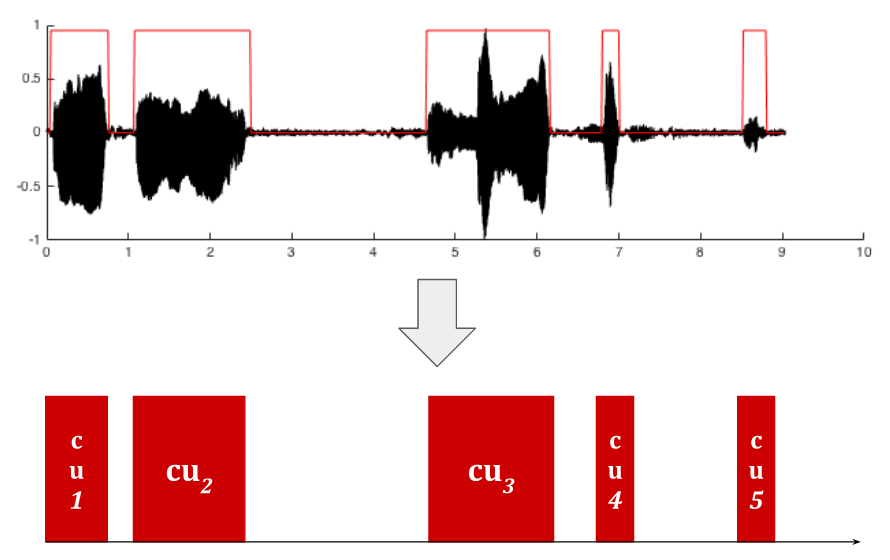
\includegraphics[width=0.6\textwidth]{bilder/vad_introduction02.png}
	\caption[Markierung stimmhafter Bereiche in einem Audiosignal]{Markierung stimmhafter Bereiche in einem Audiosignal. Oben Schwarz: Das Eingangssignal $x[\;]$. Oben Rot: Klassifizierung in \emph{stimmhaft}/\emph{nicht stimmhaft}. Unten Rot: Fünf erkannte Schreieinheiten $cu_1 , \ldots , cu_5$.}
	\label{img:vad01}
\end{figure}

In \autoref{sec:vad_new} wird die \emph{Voice Activity Detection} vorgestellt. In \autoref{sec:marking_cry-units_new} wird besprochen, wie stimmhafte Signalbereiche zu Schreieinheiten zusammengefasst werden. In \autoref{sec:decision_smoothing_new} wird ein Algorithmus vorgestellt, durch den inkorrekt erkannte Anfangs- und Endzeitpunkt von Schreieinheiten nachträglich korrigiert werden.

\section{Automatisierte Erkennung von Stimmaktivität in Signalen}
\label{sec:vad_new}

\emph{Voice Activity Detection} (kurz \emph{VAD}) oder \emph{Speech Detection}, die Feststellung des Vorhandenseins von Stimme in Signalbereichen, ist bei jeder Art der Sprachverarbeitung von Bedeutung: Im Mobilfunk wird sie beispielsweise eingesetzt, um die Zeitbereiche zu Erkennen, in denen Teilnehmer nicht sprechen und somit keine Übertragung stattfinden muss. Die größte Herausforderung von VAD-Systemen ist die robuste Erkennung von Stimmaktivität auch bei starkem Hintergrundrauschen. Bis heute wurde keine fehlerfreie Lösung für das Problem gefunden. \cite[S. 1]{vad_granada} \cite[S. 1]{vad_kola} \cite[S. 1]{vad_Lisboa}

Der Grundlegende Aufbau eines VAD-Algorithmus ist wie folgt. \autoref{img:vad_pipeline} visualisiert diesen Aufbau.
\begin{enumerate}
	\item \textbf{Vorverarbeitung} (engl. \emph{Pre-Proccessing}) des Signals.
	\item \textbf{Windowing: } Unterteilung des Signals in (einander überlappende) Signalfenster.
	\item \textbf{Extraktion von Eigenschaften} (engl. \emph{Feature-Extraction}) für jedes Signalfenster.
	\item \textbf{Entscheidung} (engl. \emph{Decision}) über die Präsens oder Abwesenheit von Stimme für jedes Signalfenster auf Grundlage der extrahierten Eigenschaften.
	\item \textbf{Entscheidungs-Glättung} (engl. \emph{Decision-Smoothing}), das nachträgliche Hinzufügen oder Entfernen von Entscheidungen mit Hilfe kontextueller Informationen der umliegenden Entscheidungen.\cite[S. 8 - 9]{vad_granada} \cite[S. 1 - 2]{vad_kola}
\end{enumerate}

\begin{figure}[h]
	\centering
	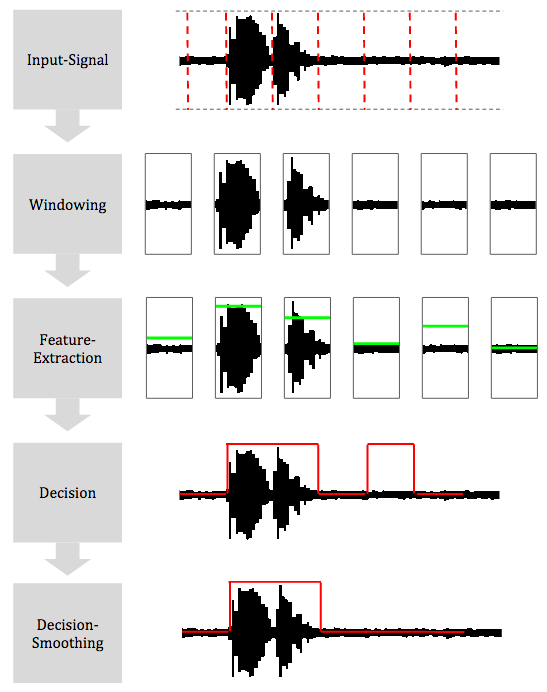
\includegraphics[width=0.6\textwidth]{bilder/vad_pipeline_04.png}
	\caption[Der grundlegende Aufbau eines VAD-Algorithmus]{Der grundlegende Aufbau eines VAD-Algorithmus (nach: \cite[S. 8]{vad_granada})}
	\label{img:vad_pipeline}
\end{figure}


In \autoref{sec:methods_vad_new} werden die Methoden vorgestellt, die zur Voice Activity Detection erprobt wurden. In \autoref{sec:vad_study} wird eine Simulationsstudie beschrieben, deren Ziel die Bestimmung derjenigen Methoden war, die sich für die VAD im speziellen Fall kindlicher Lautäußerungen am besten eignen. \autoref{sec:vad_results} fasst die Ergebnisse zusammen.

\subsection{Methoden}
\label{sec:methods_vad_new}

Die in diesem Unterabschnitt vorgestellten Methoden kombinieren Ideen, die von Moattar et al. \cite{vad_Easy}, Kristjansson et al. \cite{vad_Lisboa}, Waheed et al. \cite{vad_entropy}, Ahmadi et al. \cite{vad_ceps} und Shen et al. \cite{vad_entropie02} vorgestellt wurden.

\subsubsection{Einschränkung der zeitlichen Dynamik zur Vorverarbeitung}
\label{sec:preprocessing}

Bei der Vorverarbeitung werden Störeinflüsse auf das Signal minimiert, um die nachfolgenden Verarbeitungsschritte zu erleichtern. Welche Vorverarbeitung durchgeführt wird, ist abhängig von der konkreten Aufgabenstellung. Dieser Schritt ist für die VAD optional. So schlagen beispielsweise Ahmadi et al. \cite{vad_ceps} einen Bandpassfilter für die Vorverarbeitung vor, während Moattar et al. \cite{vad_Easy} keine Vorverarbeitung anwenden. 

In dieser Arbeit wurde sich für eine Vorverarbeitung entschieden, bei der das Signal hinsichtlich seiner Dynamik im Zeitbereich eingeschränkt wird. Dies ist ein typischer Vorverarbeitungsschritt bei Sprachaufnahmen. So wird vermieden, dass die durchschnittliche Energie des Signals für eine Erkennung der Stimmaktivität zu niedrig ist. Ein Grund für eine niedrige durchschnittliche Energie des Signals trotz maximaler Aussteuerung sind sehr kurze Pegelspitzen, deren Pegel weit über dem Durchschnittspegel liegen und so eine weitere Erhöhung der Lautstärke verhindern.\cite[S. 1 - 2]{schottland_comp}

Die Dynamikeinschränkung orientiert sich an der Arbeitsweise von Audiokompressoren. Dabei werden Signalspitzen, die über einen festgelegten \emph{Schwellwert} (engl. \emph{Threshold}) $\theta$ liegen, um ein festgelegtes \emph{Verhältnis} (engl. \emph{Ratio)} $\rho$ verringert. Ein Schwellwert von $\theta = 0.3$ mit einem Verhältnis von $\rho = 0.5$ bedeutet beispielsweise, dass alle Signalspitzen, die den Wert 0.3 über-, oder $-0.3$ unterschreiten, um 50\% verringert werden. Der Wert eines Samples nach der Kompression $x_{comp}[n]$ ergibt sich nach \autoref{eq:preprocessedX}.\cite[S. 400 - 401]{compressorPaper}

\begin{equation}
x_{comp}[n] =
\begin{cases}
\theta + (x[n] - \theta) \rho \quad , \text{wenn } x[n] > \theta \\
-\theta + (x[n] + \theta) \rho \quad, \text{wenn } x[n] < -\theta \\
x[n] \quad \text{sonst}
\end{cases}
\label{eq:preprocessedX}
\end{equation}

Die Amplituden hoher Signalspitzen werden so verringert und Headroom gewonnen, welcher anschließend bei der gleichmäßigen Erhöhung aller Amplituden zur Erhöhung der insgesamten Energie genutzt werden kann. \cite[S. 400 - 401]{compressorPaper}
    Diese Erhöhung kann beispielsweise durch eine Normalisierung nach \autoref{eq:normalizing} durchgeführt werden.

\begin{equation}
\text{normalize}(x_{comp}[n]) = \frac{x_{comp}[n]}{\maxi\{|x_{comp}[\;]|\}}
\label{eq:normalizing}
\end{equation}

In der Vorverarbeitung werden Threshold und Ratio nach \autoref{eq:THold} als Funktion des RMS-Wertes des Signals berechnet. Der Parameter $r_a$ gibt einen Ziel-RMS-Wert an.

\begin{equation}
\theta(x[\;]) = \rho(x[\;])  = \bigg[\frac{\text{RMS}(x[\;])}{r_a}\bigg]^{2}
\label{eq:THold}
\end{equation}

Die Vorverarbeitung eines Signals wird durchgeführt, indem 1.) die Kompression mit den Parametern nach \autoref{eq:preprocessedX} und 2.) die Normalisierung nach \autoref{eq:normalizing} durchgeführt wird. \autoref{img:compressing01} zeigt ein Signal vor und nach der Vorverarbeitung nach diesem Prinzip für $r_a = 0.18$ . Um eine zu große Beeinflussung des Signals zu vermeiden, wurde ein Minimalwert für Threshold und Ratio von $0.4$ festgelegt.

\begin{figure}[h]
	\centering
	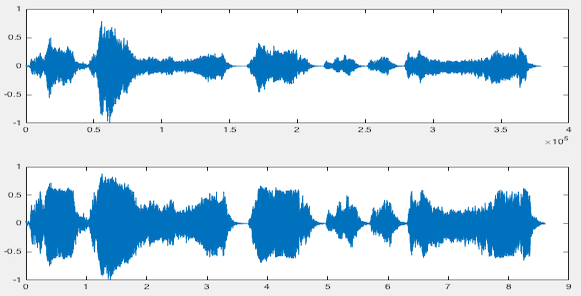
\includegraphics[width=0.6\textwidth]{bilder/compressing01.png}
	\caption[Vorverarbeitung der Voice Activity Detection]{Vorverarbeitung der Voice Activity Detection. Oben: Ein Beispielsignal vor der Vorverarbeitung. Unten: Das Beispielsignal nach der Vorverarbeitung.}
	\label{img:compressing01}
\end{figure}

Diese Vorverarbeitung eignet sich nicht für ein kontinuierliches System, da zur Berechnung des RMS-Wertes alle Samples des Signals bereits bekannt sein müssen. Das Hauptziel dieser Vorverarbeitung war die Gewährleistung ähnlicher Energieverhältnisse bei den Signalen des Trainingsdatensatzes, die in der Simulationsstudie in \autoref{sec:vad_study} verwendet wurden. Dabei wurde $r_a = 1.8$ festgelegt. Das folgende Vorgehen für den Einsatz dieser Vorverarbeitung in einem kontinuierlichen System wird vorgeschlagen:
\begin{itemize}
	\item Komplettes Überspringen der Vorverarbeitung, indem mit Hilfe eines manuell einstellbaren Lautstärkereglers eine ausreichende Signalenergie gewährleistet wird. Würde man beispielsweise anstelle der Analyse des Audiosignals ein Videosignal zur Schmerzbewertung des Gesichtsausdrucks verwenden, wäre eine Ausreichende Bildhelligkeit eine Voraussetzung für die Bilderkennung.
	\item Die Initialisierung des Kompressor mit \grqq sanften Werten\grqq , wie zum Beispiel $\theta = \rho = 0.7$. Diese Parameter können nach der Beendigung eines Schrei-Segmentes (siehe \autoref{sec:segmenting}) auf Basis des RMS-Wertes des Segmentes aktualisiert und für die Vorverarbeitung der darauf folgenden Signalbereiche eingesetzt werden.
\end{itemize}

\subsubsection{Zerlegung des Signals in überlappende Fenster}
\label{sec:windowing}

Angenommen, man führt die Voice Activity Detection für das Signal $x[\;]$ durch und kommt zu dem Schluss, dass in dem Signal (teilweise) Stimme enthalten ist. Ist das Signal mehrere Minuten oder sogar Stunden lang, ist allein aus diesem Schluss nicht ersichtlich, in welchen Zeitbereichen des Signals Stimme enthalten ist, und in welchen nicht. Um die zeitliche Auflösung zu erhöhen, wird das Signal in kürzere Zeitfenster zerlegt.

Nach der Vorverarbeitung wird diese Zerlegung mit Hilfe der in \autoref{sec:stft} als \emph{Windowing} bezeichneten Methode durchgeführt. Das Signal $x[\;]$ wird nach \autoref{eq:signal-Window} in die Signalfenster $x_0[\;] , \ldots , x_m[\;]$ aufgeteilt. Die Zeitfenster werden zunächst im Zeitbereich belassen. Es wurde sich für die von Waheed et al. \cite{vad_entropy} vorgeschlagene Fensterlänge von \SI{25}{\milli\second} entschieden, als Kompromiss zwischen den von Moattar et al. \cite{vad_Easy} empfohlenen \SI{10}{\milli\second} und den von Ahmadi et al. \cite{vad_ceps} empfohlenen \SI{40}{\milli\second}. Die Fenster überlappen einander um 50\%, das heißt \SI{12.5}{\milli\second}.

Die Entscheidung über das Vorhandensein von Stimme wird \emph{einzeln} für jedes der Signalfenster $x_0[\;] , \ldots , x_m[\;]$ durchgeführt. Grundlage für die Entscheidung ist eine Menge an Attributen, die für das jeweilige Signalfenster $x_i[\;]$ berechnet wird. Die Ermittlung und Evaluation geeigneter Attribute ist einer der primären Forschungsbereiche in der VAD. In den folgenden Unterabschnitten \ref{sec:vad_time_features} bis \ref{sec:vad_dif_feature} wird eine Reihe an Features vorgestellt, die in dieser Arbeit zur VAD erprobt wurden. Jedes der in diesen Unterabschnitten besprochenen Features kann für ein Signalfenster $x_i[\;]$ \`{a} \SI{25}{\milli\second} berechnet werden und als Grundlage für eine Entscheidung dienen. Die Evaluation dessen, welche Attribute sich am besten als Entscheidungsgrundlage zur Feststellung von Babylauten eignen, folgt in \autoref{sec:vad_study}. Die Ergebnisse werden in \autoref{sec:vad_results} zusammengefasst.

\subsubsection{Eigenschaften des Zeitbereiches}
\label{sec:vad_time_features}

Im Zeitbereich wurden die beiden Eigenschaften \emph{Root Mean Square} [\emph{RMS}] und \emph{Zero Crossing Rate} [\emph{ZCR}] erprobt.

Moattar et al. \cite[S. 2549]{vad_Easy} bezeichnen den Energiegehalt eines Signals als das für die VAD am häufigsten angewandte Attribut. Der RMS-Wert als Feature für ein Signalfenster wird nach \autoref{eq:rms} berechnet. Hintergrund ist, dass der Energiegehalt eines Stimmsignals typischerweise höher ist als der des Hintergrundrauschens. Bei geringem Signal-Rausch-Abständen ist diese Bedingung jedoch nicht immer erfüllt. Als zweites Attribut des Zeitbereiches wurde die \emph{Zero Crossing Rate} nach \autoref{eq:zcr} berechnet. Dieses Feature misst die Häufigkeit eines Vorzeichenwechsels im Signal. Stimmlose Signalbereiche haben typischerweise eine höhere ZCR als stimmhafte Signalbereiche. Problematisch ist dieses Kriterium bei Signalen, bei denen kein Hintergrundrauschen vorliegt, da sich dort eine ZCR von 0 ergibt.\cite[S. 335 - 336]{vad_ceps} Um den Wert in Relation zur Fensterlänge setzen zu können, wird die ZCR durch die Anzahl der Samples eines Signalfensters $N$ geteilt.

\begin{equation}
\text{ZCR}(x_i[\;]) = \sum_{0}^{N-1}|\text{sng}(x_i[n])-\text{sng}(x_i[n-1])|
\label{eq:zcr}
\end{equation}

\subsubsection{Eigenschaften der Autokorrelation}

Neben dem RMS-Wert und der ZCR wurde die Autokorrelation zur VAD erprobt. Die Autokorrelation eignet sich, um Periodizität in einem Signal nachzuweisen. Wie in \autoref{sec:theVoice} erläutert wurde, weisen stimmhafte Signale ein tendenziell stärker periodisches Verhalten als stimmlose Signalteile auf. 

Bei der Autokorrelation wird ein Signal mit einer verzögerten Variante von sich selbst korreliert. \autoref{eq:ACorr} definiert die Autokorrelation des $N$-Sample langen Signalfensters $x_i[\;]$, verzögert um einen als \emph{Lag} bezeichneten Wert $k$.\cite[S. 1]{vad_Lisboa}

\begin{equation}
\text{A-Corr}_k(x[\;]) = \sum_{n=k}^{N} x[n-k] \cdot x[n]
\label{eq:ACorr}
\end{equation}

Da der Autokorrelationswert neben der Stärke der Periodizität von der Signalenergie abhängig ist, ist eine Normalisierung des Wertes wünschenswert. Es gibt verschiedene Varianten dieser Normalisierung. \autoref{eq:NACorr} definiert die \glqq normalisierte Autokorrelation\grqq{}, bei der der Autokorrelationswert durch die RMS-Werte des verzögerten und des unverzögerten Signals normalisiert wird. Ein hoher Wert der normalisierten Autokorrelation mit der Verzögerung $k$ spricht für eine ausgeprägte Periodizität des Signals mit der Frequenz $f =  f_s / k $.\cite[S. 1 - 2]{vad_Lisboa}

\begin{equation}
\text{NA-Corr}_k(x[\;]) = \frac{\sum_{n=k}^{N} x[n-k] \cdot x[n]}{ \sqrt{\sum_{n=1}^{N-k}  x[n]^2}  \cdot  \sqrt{\sum_{n=k}^{N}  x[n]^2} }
\label{eq:NACorr}
\end{equation}

%Das Autokorrelations-Signal $a[\;]$ wird erstellt, indem die normalisierte Autokorrelation für verschiedene $k = k_{min} , \ldots , k_{max}$ angewandt wird, wie Gleichung \ref{eq:a-Signal} definiert. 

%\begin{equation}
%a[\;] := \quad \mathop{\forall}_{k = k_{min}}^{k_{max}} :\ a[k] = \text{NA-Corr}_k(x[\;]) 
%\label{eq:a-Signal}
%\end{equation}

In Bezug auf die VAD wurde die Autokorrelation als Methode genutzt, um die beiden Attribute \emph{höchste Autokorrelationsspitze} [\emph{aMax}] und \emph{Anzahl der Autokorrelationsspitzen} [\emph{aCount}] zu berechnen. Beide Eigenschaften wurden von Kristjansson et al. \cite[S. 1 - 2]{vad_Lisboa} zur VAD beschrieben. Die \emph{höchste Autokorrelationsspitze} wird in \autoref{eq:corrpeak} definiert und bestimmt die höchste Magnitude der normalisierten Autokorrelation für die Verzögerungswerte $k_{min} , \ldots , k_{max}$. Ein stimmhaftes Signal hat aufgrund seiner Periodizität erwartungsgemäß einen höheren [\emph{aMax}]-Wert als Rauschen.

\begin{equation}
\text{aMax}(x_i[\;]) = \maxmagi_{k = k_{min} \: \ldots \: k_{max}}\{\text{NA-Corr}_k(x_i[\;])\}
\label{eq:corrpeak}
\end{equation}

Die \emph{Anzahl der Autokorrelationsspitzen} wird nach \autoref{eq:corrcount} berechnet. Das Feature gibt an, wie viele Signalspitzen im Autokorrelationssignal enthalten sind. Rauschen erzeugt höhere [\emph{aCount}]-Werte als stimmhafte Signale, bedingt durch die vielen zufällig verteilten Periodizitäten.\cite[S. 1 - 2]{vad_Lisboa}

\begin{equation}
\text{aCount}(x_i[\;]) = \counti_{k = k_{min} \: \ldots \: k_{max}}\{\text{NA-Corr}_k(x_i[\;])\}
\label{eq:corrcount}
\end{equation}

Das Verzögerungsintervall $k_{min} , \ldots , k_{max}$ wurde so gewählt, dass Periodizitäten nur in dem Bereich gesucht wurden, der für die Grundfrequenz von Babystimmen in Frage kommt. Aus \autoref{sec:acousticModel} ging hervor, dass diese Grundfrequenz für Babys zwischen $250$ und $\SI{2000}{\hertz}$ liegt.

\subsubsection{Eigenschaften des Frequenzbereiches}

auf Basis des Frequenzbereiches wurden die drei Eigenschaften \emph{unnormalisierte spektrale Entropie} [$SEnt_{u}$], \emph{normalisierte spektrale Entropie}  [$SEnt_{n}$] und \emph{dominanteste Frequenzkomponenten} [$f_{dom}$] erprobt.\cite{vad_Lisboa}

Als Vorbereitungsschritt wird das Signalfenster des Zeitbereiches $x_i[\;]$ in den Frequenzbereich $X_i[\;]$ transformiert. Die Berechnungsvorschrift ist $X_i[\;] = \text{DFT}\{(w[\;] \cdot x_i[\;])\}$. Wird diese Transformation für alle Signalfenster $x_0[\;], \ldots, x_m[\;]$ durchgeführt, entspricht dies der in \autoref{sec:stft} vorgestellten Kurzzeit-Fourier-Transformation des ursprünglichen Eingangssignals $x[\;]$. Es wurde eine $2048$ Punkte lange FFT und ein Hamming-Window als Fensterfunktion $w[\;]$ verwendet.

Kristjansson et al. \cite[S. 2]{vad_Lisboa} haben die \emph{spektrale Entropie} zur VAD beschrieben. Dabei wird das Spektrum des Frequenzfensters $X_i[\;]$ als Wahrscheinlichkeitsverteilung betrachtet. Die Entropie als Maß zur \glqq Unreinheit\grqq{} wurde in \autoref{sec:id3} erläutert. Die \emph{normalisierte spektrale Entropie} wird nach der \autoref{eq:norm_se} berechnet. Das Signal $px_i[\;]$ ergibt sich durch die Normalisierung des $N$-Punkte langen Spektrums nach \autoref{eq:norm_spek}. Bei der normalisierten spektralen Entropie ist zu erwarten, dass Frequenzfenster ohne Stimme einen höheren Wert aufweisen als Fenster mit Stimme.\cite[S. 2]{vad_Lisboa} 

\begin{equation}
px_i[n] = \frac{X_i[n]}{\sum_{k=1}^{N} X_i[k]}
\label{eq:norm_spek}
\end{equation}

\begin{equation}
\text{SEnt}_n(px_i[\;]) = -\sum_{k=1}^{N}px_i[k] \cdot\log(px_i[k])
\label{eq:norm_se}
\end{equation}

Neben der von Kristjansson et al. \cite{vad_Lisboa} vorgestellten normalisierten spektralen Entropie wurde zusätzlich die \emph{unnormalisierte Spektrale Entropie} nach \autoref{eq:unnnorm_se} berechnet. Bei dieser wird das Spektrum nicht normalisiert, das heißt, es gilt $px_i[k] = X_i[k]$. Somit hat die Energie des Signals einen größeren Einfluss auf den Wert des Attributes. Dabei ist zu erwarten, dass Signalfenster mit Stimme einen höheren Wert aufweisen als solche mit Rauschen.

%\footnote{Kristjansson et al \cite[S. 2]{vad_Lisboa} verwenden zur Entropie-Berechnung den Logarithmus zur Basis 10, anstatt zur Basis 2. Es ist nicht klar, ob es sich dabei um einen Fehler handelt. In dieser Arbeit wurde, wie in der Publikation beschrieben, ebenfalls der Logarithmus zur Basis 10 verwendet.}

\begin{equation}
\text{SEnt}_u(X_i[\;]) = -\sum_{k=1}^{N}X_i[k] \cdot\log(X_i[k])
\label{eq:unnnorm_se}
\end{equation}

In die Berechnungen wurden nur die Frequenzen im Bereich von 250 - \SI{8000}{\hertz} mit einbezogen, da nach \autoref{sec:acousticModel} die tiefst mögliche Grundfrequenz einer Babystimme bei \SI{250}{\hertz} liegt und nach Shen et al. \cite{vad_entropie02} die Stimme keine Informationen oberhalb von \SI{8000}{\hertz} enthält.

Moattar et al. \cite[S. 2550]{vad_Easy} haben die \emph{dominanteste Frequenzkomponente} zur VAD vorgestellt. Für jedes Frequenzfenster $X_i[\;]$ wird diejenige Frequenz nach  \autoref{eq:domfreq} berechnet, welche die höchste Amplitude hat. Es wird dabei, im Gegensatz zur spektralen Entropie, der gesamte Frequenzraum betrachtet. Ein stimmhaftes Signal hat typischerweise eine höhere $f_{dom}$ als ein stimmloses Signal, bedingt durch die hohe Amplitude der Grundfrequenz.\cite[S. 2550]{vad_Easy}

\begin{equation}
f_{dom}(X_i[\;]) = \argmax \{X_i[\;]\}
\label{eq:domfreq}
\end{equation}


\subsubsection{Eigenschaften des Cepstrums}
\label{sec:vad_ceps_features}

Das Cepstrum wird nach \autoref{eq:cepstrum} als die inverse DFT des Logarithmus des Magnitudensignals des Frequenzbereiches definiert.\cite[\emph{Cepstral Analysis}, S. 2]{ricardo_ceps}

\begin{equation}
c[\;] =  \text{iDFT}\Big\{ \log \Big(\ \big|\ \text{DFT}\{x[\;]\} \big|\ \Big) \Big\}
\label{eq:cepstrum}
\end{equation}	

\begin{figure}[h]
	\centering
	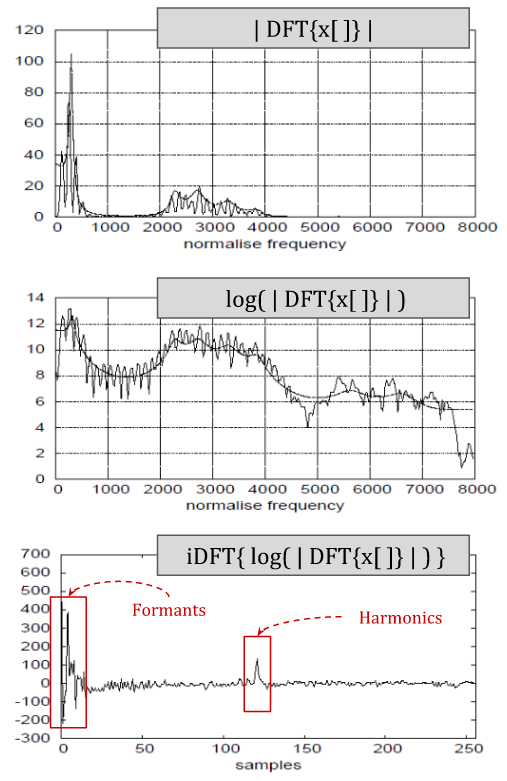
\includegraphics[width=0.55\textwidth]{bilder/cepstrum04.png}
	\caption[Berechnung des Cepstrums]{Berechnung des Cepstrums. (nach: \cite[\emph{Cepstral Analysis}, S. 3]{ricardo_ceps})}
	\label{img:cepstrumOverview}
\end{figure}

Das Vorgehen wird mit Hilfe des Beispiels aus \autoref{img:cepstrumOverview} erläutert. $ |\ \text{DFT}\{x[\;]\}\ \big| $  zeigt das Spektrum eines \glqq typischen stimmhaften\grqq{} Signals $x[\;]$. Es sind die in \autoref{sec:theVoice} erläuterten, für ein stimmhaftes Signal typischen harmonischen Obertöne zu sehen, welche mit steigender Frequenz an Amplitude verlieren. Durch das Logarithmieren des Spektrums $\log \big(\ |\ \text{DFT}\{x[\;]\} |\ \big)$ wird die Dynamik des Frequenzbereiches verringert und somit der Amplitudenverlust der höheren Obertöne reduziert. Man stelle sich vor, dieses Spektrum wäre ein Signal des Zeitbereiches. In diesem Fall würde man die harmonischen Obertöne als ein annähernd periodisches Signal betrachten, welches von einem niederfrequenten Signal überlagert wird. Um diese beiden Frequenzkomponenten voneinander zu trennen, müsste man eine weitere DFT anwenden. Diese DFT kommt in dem Fall einer inversen DFT gleich, da das Phasen-Signal verworfen wurde. Man erwartet in diesem \glqq Spektrum vom Spektrum\grqq{} eine Signalspitze im \glqq oberen Frequenzbereich\grqq , bedingt durch die harmonischen Obertöne, sowie eine Signalspitze im \glqq unteren Frequenzbereich\grqq, bedingt durch die Formanten.\cite[\emph{Cepstral analysis}, S. 4]{ricardo_ceps}

Der Bereich dieser \glqq Fourier-Transformation der Fourier-Transformation\grqq{} wird als \emph{Cepstrum} bezeichnet. Cepstrum ist ein ein Wortspiel, welches durch die Umkehrung der ersten vier Buchstaben des Wortes \glqq Spectrum\grqq{} entsteht. Die unabhängige Variable des Cepstrum wird als \emph{Quefrency} bezeichnet. So wird verdeutlicht, dass die unabhängige Variable dieses Bereichs zwar mathematisch betrachtet die Zeit darstellt, jedoch als Frequenz interpretiert wird.\cite[\emph{Cepstral analysis}, S. 7]{ricardo_ceps}	

Ein Aufkommen einer Signalspitze im oberen Quefrency-Bereich $> \SI{3}{\milli\second}$ spricht für das Vorhandensein von harmonischen Obertönen im Signal, wie sie beispielsweise durch Stimme erzeugt werden. \autoref{img:cepstrumVoicedPeak} verdeutlicht das Prinzip an einem Beispiel. Zu sehen ist die Kurzzeit-Fourier-Transformation eines Signals mit einer Fensterlänge von $\SI{50}{\milli\second}$ und einer Hopsize von $\SI{12.5}{\milli\second}$. Links wird das logarithmierte Spektrum des entsprechenden Frequenzfensters abgebildet, rechts das Cepstrum. Die Frames 1 bis 5 sind stimmlos und die Frames 8 bis 15 sind stimmhaft. Die Frames 6 und 7 bilden eine Zwischenform zwischen stimmhaft und nicht-stimmhaft. Wie zu sehen ist, haben die Cepstren der stimmhaften Frames eine Signalspitze bei der Quefrency $q \approx \SI{12}{\milli\second}$.\cite[\emph{Cepstral Analysis}, S. 16]{ricardo_ceps}

\begin{figure}[h]
	\centering
	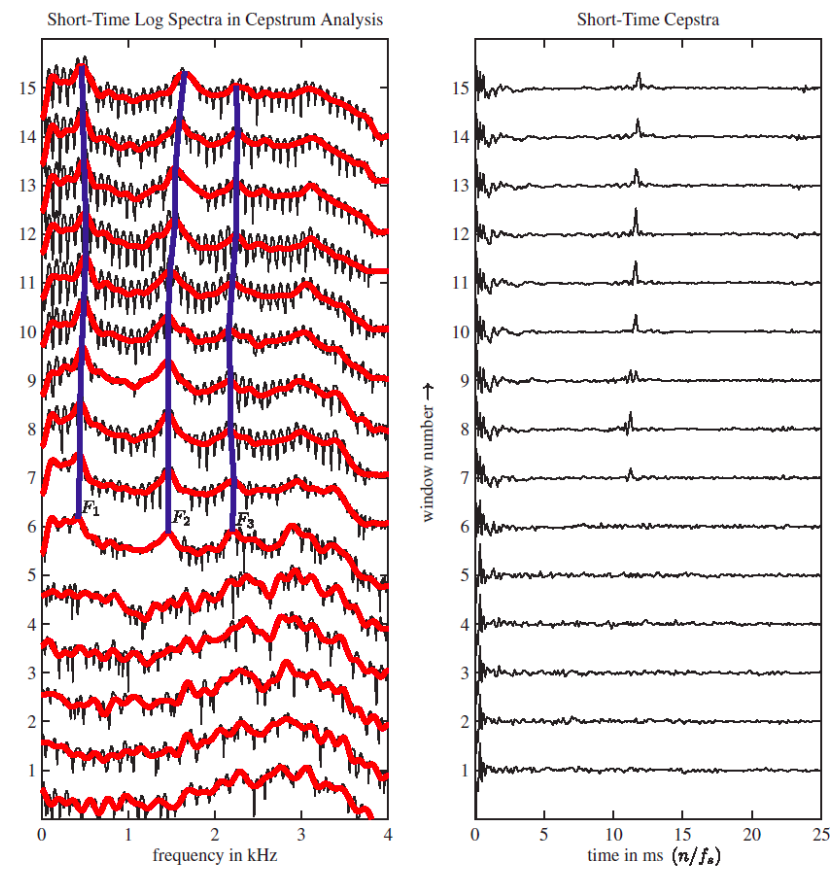
\includegraphics[width=0.6\textwidth]{bilder/cepstrum05.png}
	\caption[Aufkommen einer Signalspitze im oberen Quefrency-Bereich]{Aufkommen einer Signalspitze im oberen Quefrency-Bereich bei stimmhaften Signalfenstern. \cite[\emph{Cepstral Analysis}, S. 17]{ricardo_ceps}}
	\label{img:cepstrumVoicedPeak}
\end{figure}

\autoref{img:cepstrumPitch} verdeutlicht, wie eine Periode von $T_0$ im Zeitbereich eine Signalspitze im Frequenzbereich bei der Grundfrequenz $f_0$ bedingt, welche wiederum in Verbindung mit den harmonischen Obertönen eine Signalspitze bei der Quefrency $q_o = 1 / f_0$ im Cepstrum verursacht. Wird somit in einem Cepstrum eine Signalspitze bei $q_0$ festgestellt, weißt dies auf eine Grundfrequenz von $f_0 = 1/q_0$ hin. \cite[S. 5]{cepstrumPitchTranslation}

In Bezug auf die VAD wurde das Cepstrum genutzt, um die beiden Features \emph{Höchster Peak im Cepstrum} [$Ceps_{mag}$] und \emph{Quefrency des höchsten Peaks} [$Ceps_{loc}$] zu berechnen.

Ahmadi et al. \cite{vad_ceps} sowie Kristjansson et al. \cite{vad_Lisboa} schlugen vor, die Magnitude der höchsten Signalspitze im oberen Bereich des Cepstrums als Maß für die Stimmhaftigkeit eines Signals einzusetzen. \autoref{eq:ceps_maxpeak} definiert die Berechnung dieses Attributs. $c_i[\;]$ ist das Cepstrum des $i$-ten Frequenzfensters $X_i[\;]$. So wie bei den Attributen der Autokorrelation wurde, entsprechend den möglichen Grundfrequenzen von Babystimmen, ein Quefrency-Bereich von $q_{min} = 5$ bis $q_{max} = \SI{40}{\milli\second}$ durchsucht.

\begin{equation}
Ceps_{mag}(c_i[\;]) = \maxmagi_{q = q_{min} \ldots , q_{max}}\{ \; c_i[q] \; \}
\label{eq:ceps_maxpeak}
\end{equation}

Als zweites Attribut, welches auf dem Cepstrum basiert, wurde die Quefrency der höchsten Amplitude des oberen Quefrency-Bereiches nach \autoref{eq:ceps_loc} berechnet. Bei Signalfenstern ohne Stimme ist es wahrscheinlicher, dass sich die höchste Amplitude am Mindest- oder Maximalwert des durchsuchten Quefrency-Bereiches befindet.

\begin{equation}
Ceps_{loc}(c_i[\;]) = \argmax_{q = q_{min} \ldots , q_{max}} \{ \; c_i[q] \; \}
\label{eq:ceps_loc}
\end{equation}	

\begin{figure}[h]
	\centering
	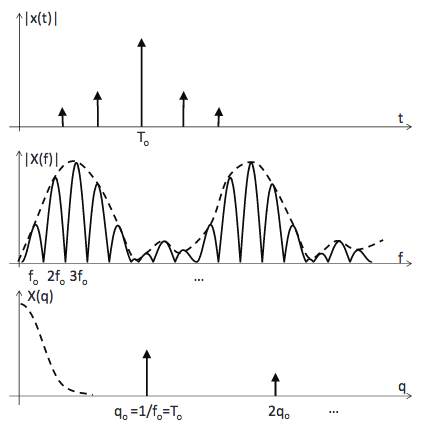
\includegraphics[width=0.5\textwidth]{bilder/cepstrumPitch.png}
	\caption[Feststellung der Grundfrequenz aus dem Cepstrum]{Feststellung der Grundfrequenz aus dem Cepstrum \cite[S. 5]{cepstrumPitchTranslation}}
	\label{img:cepstrumPitch}
\end{figure}

\subsubsection{Differenz-Features}
\label{sec:vad_dif_feature}

\autoref{img:vadAllFeatures} visualisiert alle Attribute, die in den vorangegangenen Unterabschnitten zur VAD vorgestellt wurden. Der oberste Plot zeigt das Audiosignal aus \autoref{img:vad01} mit einem Signal-Rausch-Abstand von \SI{20}{\decibel}. Die rote Linie des obersten Plots klassifiziert die Zeitbereiche in $1 \; \hat{=} $ \emph{stimmhaft} und $0 \; \hat{=}$ \emph{nicht stimmhaft}. Alle darunter liegenden Plots zeigen den zeitlichen Verlauf der entsprechenden Attribute.

\autoref{img:min-signal} zeigt den zeitlichen Verlauf des RMS-Features im Detail. (A) zeigt das verhalten des \emph{RMS}-Attributes bei einem Signal-Rausch-Abstand von \SI{50}{\decibel}. Die stimmlosen Zeiträume haben einen weitaus niedrigeren RMS-Wert als die Zeiträume mit Stimme. In (B) ist das selbe Signal mit einem Signal-Rausch-Abstand von \SI{3}{\decibel} zu sehen. Nun liegen die RMS-Werte der stimmlosen Bereiche nur noch knapp unter denen des Sprachsignals. Zu sehen ist, dass starkes Hintergrundrauschen ähnlich hohe Feature-Werte erzeugen kann wie die Stimme.

\begin{figure}[H]
	\centering
	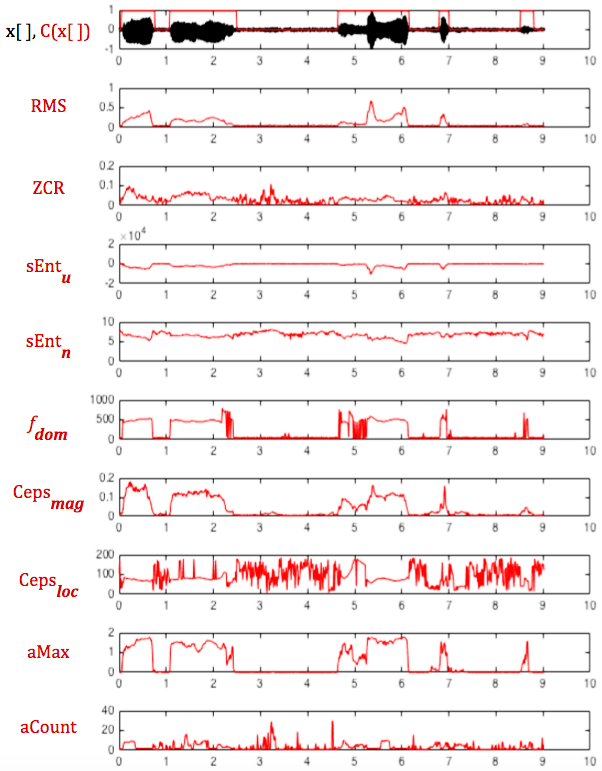
\includegraphics[width=0.85\textwidth]{bilder/allFeatures03.png}
	\caption[Übersicht über alle Attribute, die für die VAD erprobt wurden]{Übersicht über alle Attribute, die für die Voice Activity Detection erprobt wurden.}
	\label{img:vadAllFeatures}
\end{figure}

Moattar et al. \cite{vad_Easy} und Waheed et al. \cite{vad_entropy} schlugen vor, den Wert des jeweiligen Attributes zu messen, der in den stimmlosen Bereichen durch das Hintergrundrauschen erzeugt wird. Es kann davon ausgegangen werden, dass die ersten Signalfenster eines Signals stimmlos sind, und der Feature-Wert des Rauschens somit anhand dieser Fenster bestimmt werden kann. Bei einer langanhaltenden und kontinuierlichen Analyse können sich sowohl der Signal-Rausch-Abstand als auch die Qualität des Rauschens ständig ändern, weshalb in von den stimmlosen Bereichen erzeugten Attributwerte regelmäßig aktualisiert werden müssen. Es kann weiterhin davon ausgegangen werden, dass die Länge einer Cry-Unit eine bestimmte Länge $t_{max}$ nicht überschreiten kann, bevor das Baby Luft holen muss und somit mindestens ein stimmloses Zeitfenster entsteht, welches das Hintergrundrauschen enthält. Zeskind et al. \cite[S. 325]{rythmic} haben $t_{max} = \SI{4.75}{\second}$ bestimmt. In einem Zeitbereich $ t > t_{max}$ muss somit zumindest ein Feature-Wert enthalten sein, der durch stimmlose Singalbereiche erzeugt wurde. 

\begin{figure}[h]
	\centering
	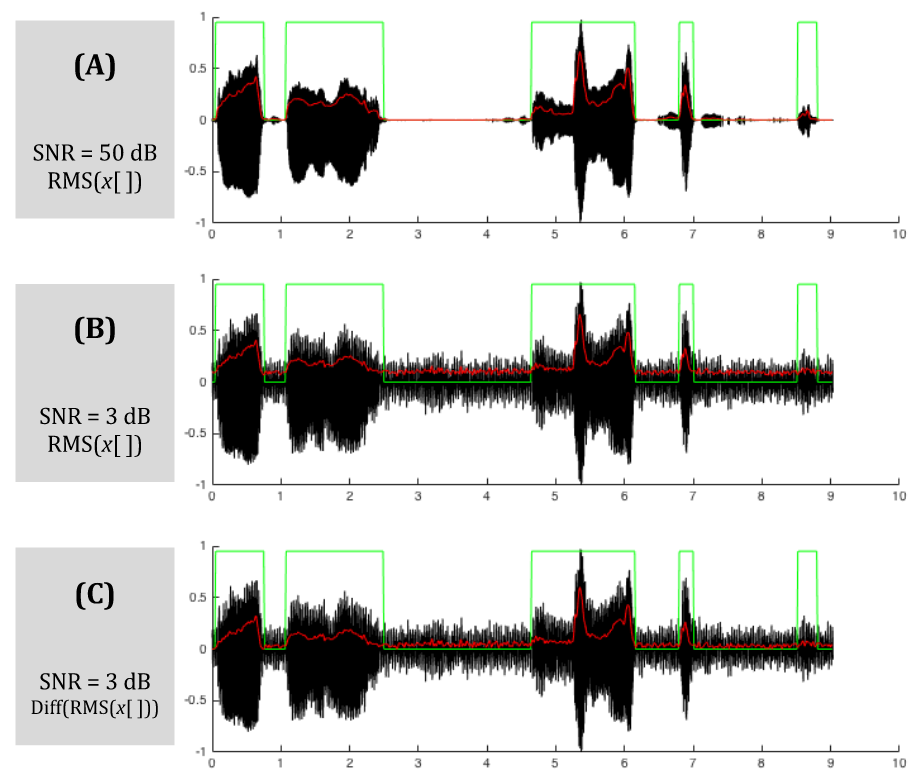
\includegraphics[width=0.7\textwidth]{bilder/rms_diff.png}
	\caption[Das RMS-Feature bei verschiedenen Signal-Rausch-Abständen]{Das RMS-Feature bei verschiedenen Signal-Rausch-Abständen. Schwarz: Eingangs-Signal $x[\;]$. Grün: Klassifizierung in \emph{stimmhaft/nicht stimmhaft}. Rot: zeitlicher Verlauf des RMS-Features.}
	\label{img:min-signal}
\end{figure}

Auf Basis dieser Überlegung wurde das \emph{Differenz-Feature} Diff\textsubscript{t}(Feat$(x_i[\;])$) nach \autoref{eq:difFeature} definiert als die Differenz zwischen einem aktuell gemessenen Attributwerte und dem geringsten Attributwerte, welcher im vergangenen Zeitbereich $t$ gemessen wurde. Feat$(x_i[\;])$ bezeichnet dabei einen beliebigen Feature-Wert des Signalfensters $x_i[\;]$, $t_{xi}$ die Länge eines Signalfensters in Sekunden (in diesem Fall \SI{25}{\milli\second}), und $t$ den zu durchsuchende Zeitbereich in Sekunden $> t_{max}$, welcher von dem jeweiligen Signalfenster $x[\;]$ aus betrachtet in der Vergangenheit liegt. In \autoref{img:min-signal} wird in (C) das Differenz-Feature für den RMS-Wertes gezeigt.

\begin{equation}
\text{Diff}_t(\text{Feat}(x_i[\;])) = \text{Feat}(x_i[\;])\ - \mini_{k=(i-z)...i}\{\text{Feat}(x_k[\;])\} \qquad , z = \frac{2 \cdot t}{t_{xi}}
\label{eq:difFeature}
\end{equation}

In dieser Arbeit wurde $t = \SI{5}{\second}$ festgelegt. Es ist zu beachten, dass die Attribute \emph{ZCR, SEnt\textsubscript{u}} und \emph{aCount} zur Berechnung des Differenz-Features bezüglich ihres Vorzeichens invertiert werden müssen, da bei ihnen niedrige an Stelle hoher Werte stimmhafte Signale anzeigen. Das einzige Attribut, für dass die Berechnung des Differenz-Features keinen Sinn macht, ist das \emph{Ceps\textsubscript{loc}}-Attribut, da es bei stimmlosen Signalabschnitten sowohl einen höheren als auch einen niedrigeren Wert annehmen kann.

\subsubsection{Entscheidung über das Vorhandensein von Stimme auf Basis der Attribute}

Eine einfache Variante zur Entscheidung darüber, ob ein Signalfenster $x_i[\;]$ Stimme enthält, ist, eines der vorgestellten Attribute als Entscheidungsgrundlage zu wählen und einen festen Grenzwert $\theta$ festzulegen, bei dessen Über- oder Unterschreitung das Fenster als stimmhaft klassifiziert wird. Die Entscheidung lässt sich als \emph{Klassifizierungsfunktion} (auch: \emph{Klassifikator}) $C: \{ x_i[\;] \} \mapsto Y$ definieren, welche ein Signalfenster abbildet auf $Y = \{ 1 \; \hat{=} \; \text{stimmhaft}, \; 0 \; \hat{=} \; \text{nicht stimmhaft}\}$. Die Klassifizierungsfunktion nimmt dann die folgende Form an:

\begin{equation}
	C(x_i[\;]) = 
\begin{cases}
1 \quad , \text{wenn Feat}(x_i[\;]) > \theta \\
0 \quad , \text{sonst}
 \end{cases}
\end{equation}

\autoref{img:thresholded} verdeutlicht das Prinzip an einem Beispiel. Das Feature, dass als Entscheidungsgrundlage genutzt wird, ist der \emph{RMS}-Wert. Ein Grenzwert von $\theta = 0.18$ gewährleistet in diesem Fall eine weitestgehend richtige Klassifizierung.

\begin{figure}[h]
	\centering
	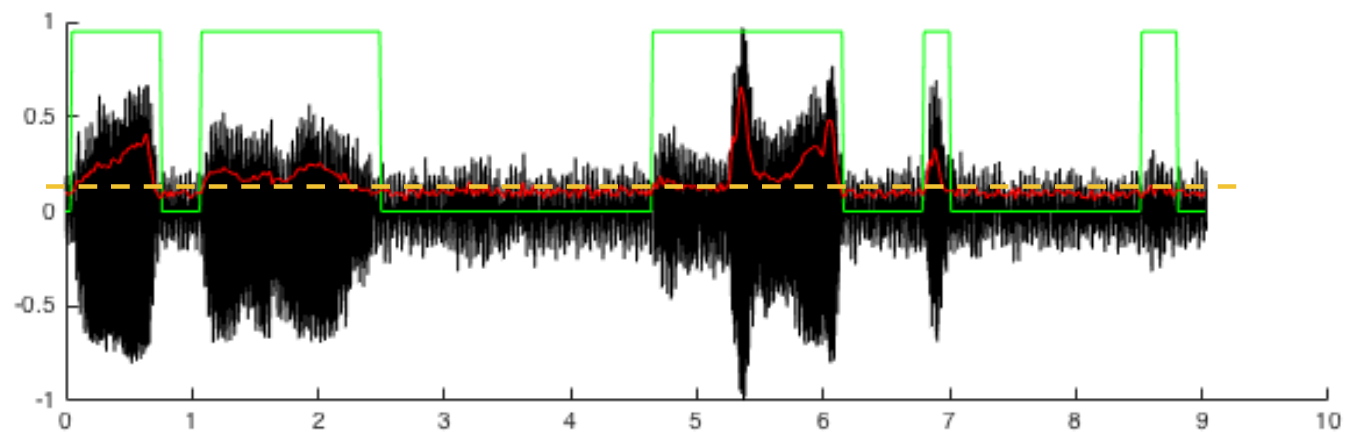
\includegraphics[width=0.65\textwidth]{bilder/thresholded02.png}
	\caption[Beispiel für die Grenzwertsetzung eines Features]{Beispiel für die Grenzwertsetzung eines Features. Schwarz: Das Eingangssignal $x[\;]$. Grün: Klassifizierung in \emph{stimmhaft/nicht stimmhaft}. Rot: RMS-Feature. Gelb: Grenzwert}
	\label{img:thresholded}
\end{figure}

Es stellt sich die Frage, wie man für ein Attribut einen Grenzwert findet, der für verschiede Signal-Rausch-Abstände eine möglichst hohe Klassifikationsgenauigkeit gewährleistet. In einigen Veröffentlichungen, so wie der von Moattar et al. \cite{vad_Easy}, wird empfohlen, den Grenzwert experimentell festzustellen. In dieser Arbeit wurde sich für den Ansatz einer automatisierten, datengetriebenen Grenzwertsuche mit Hilfe des in \autoref{sec:id3} vorgestellten \emph{C4.5}-Algorithmus entschieden. Der Grundgedanke ist wie folgt: Angenommen, man hat eine Datenbank zur Verfügung, bestehend aus einer Menge an Signalen mit Audioaufnahmen kindlicher Lautäußerungen, in denen manuell die stimmhaften Signalabschnitte markiert wurden. Diese Signale zerlegt man nach den vorgestellten Methoden in kürzere Signalfenster und berechnet für jedes Signalfenster das Feature, dessen Grenzwert man sucht. Jedes Signalfenster versieht man außerdem mit dem Klassenlabel $y \in Y$ auf Basis der manuellen Markierungen. Ein \emph{Signalfenster} $x_i[\;]$ wird so zu einem \emph{Exempel} $e_i = (\text{Feat}(x_i[\;]), y_i)$. Alle Exempel werden zu einem \emph{Trainingsdatensatz} zusammengetragen. Nun kann der \emph{C4.5}-Algorithmus verwendet werden, um für das Feature den Grenzwert zu finden, der für diesen Datensatz die Klassifizierung mit der höchsten Genauigkeit vornimmt. Voraussetzung dafür ist, dass die maximale Tiefe des zur Klassifizierung entworfenen Entscheidungsbaums mit 1 bestimmt wird, damit für das jeweilige Attribut genau ein Grenzwert festgelegt wird. Ist das Attribut, für das der Grenzwert gesucht wird, ein Differenz-Feature, so lässt sich der Grenzwert als ein adaptiver Grenzwert interpretieren, der sich an den aktuellen SNR anpasst.

%besser formulieren!
Die Verwendung des \emph{C4.5}-Algorithmus bringt die Möglichkeit mit sich, eine beliebige Menge an Features in die Klassifizierung mit einzubeziehen. Die Klassifizierung muss also nicht zwingend auf Grundlage nur eines Attributes geschehen. Angenommen, es werden die beiden Features $RMS$ und $ZCR$ für jedes Signalfenster einer Datenbank berechnet, dann enthält jedes Exempel des so konstruierten Trainingsdatensatzes diese beiden Features. Wird dieser Trainingsdatensatz dem \emph{C4.5}-Algorithmus zum Entwurf eines Klassifikators gegeben, dann nimmt der Klassifikator die Form eines Entscheidungsbaumes an, bei dem durch das hierarchische Setzen von Grenzwerten die Klassifizierung vorgenommen wird. \autoref{lst:tree01} zeigt ein Beispiel für eine so resultierenden, fiktiven Klassifikator.

\begin{lstlisting}[frame=single,mathescape=true,basicstyle=\footnotesize,language=Java,label=lst:tree01,caption=Beispiel eines Entscheidungsbaums für die Klassifizierung bei der VAD,linewidth=1\textwidth]
if RMS($x_i[\;]$) > 0.2
|   if ZCR($x_i[\;]$) < 0.13
|   |   C($x_i[\;]$) = 0
|   |else
|   |   C($x_i[\;]$) = 1
|else
|    C($x_i[\;]$) = 1
\end{lstlisting}

Wird dem \emph{C4.5}-Algorithmus eine größere Menge an Attributen zur Verfügung gestellt, auf deren Basis der Klassifikator entworfen wird, wird der Entscheidungsbaum implizit zeigen, welche Features für die VAD besser geeignet sind, da sie höher im Entscheidungsbaum erscheinen. Es besteht jedoch die Gefahr, dass der Algorithmus in ein lokales Maximum gelaufen ist und der entworfene Klassifikator somit eine suboptimale Auswahl an Features verwendet. Außerdem besteht die Gefahr des Overfitting, insofern Entscheidungsbäume mit beliebiger Tiefe zugelassen werden.

\subsection{Simulationsstudie zur Festlegung des Klassifikators}
\label{sec:vad_study}

In \autoref{sec:methods_vad_new} wurde eine Übersicht über die Methoden gegeben, die in dieser Arbeit zur VAD erprobt wurden. Neben Methoden zur Vorverarbeitung und zur Zerlegung eines Signals in kürzere Fenster wurde eine Reihe an Attributen vorgestellt, die für ein Signalfenster als Entscheidungsgrundlage für die Erkennung des Vorhandenseins von Stimme dienen können. Schlussendlich wurde erläutert, wie der \emph{C4.5}-Algorithmus genutzt werden kann, um einen Klassifikator zu entwerfen, der die Entscheidung über das Vorhandensein von Stimme auf Grundlage einer Menge von Features fällt. Dafür wird ein Datensatz zum Training des \emph{C4.5}-Algorithmus benötigt.

Das Ziel ist es nun, auf Grundlage dieser Methoden den tatsächlichen Klassifikator zu finden. Der Klassifikator soll dabei die folgenden Bedingungen erfüllen:

\begin{itemize}
\item Der Klassifikator soll eine möglichst kleine Anzahl an Features verwenden, da es rechnerisch zu aufwendig wäre, alle vorgestellten Features allein für die VAD in einem kontinuierlichen System zu berechnen.
\item Der Klassifikator soll eine möglichst hohe Genauigkeit erzielen, unabhängig von Stärke und Qualität des Hintergrundrauschens.
\end{itemize}

\pagebreak

Das Vorgehen zum Finden des Klassifikators war wie folgt:
\begin{enumerate}
\item Es wurde ein Menge an Trainingsdatensätzen erstellt, indem ...
	\begin{enumerate}[label*=\arabic*.]
	\item in einer Menge an Audioaufnahmen weinender Babys manuell die stimmhaften Signalabschnitte markiert wurden, ...
	\item diese Audioaufnahmen vorverarbeitet, in Signalfenster zerlegt und für jedes Signalfenster alle vorgestellten Features berechnet wurden, ...
	\item woraus Datensätze erzeugt wurden, wobei jeder Datensatz nur eine bestimmte Untermenge der Features zur Verfügung gestellt bekam.
	\end{enumerate}
\item Auf Basis jedes Datensatzes wurde mit Hilfe des \emph{C4.5}-Algorithmus ein Klassifikator erzeugt.
\item Jeder Klassifikator wurde bezüglich seiner Genauigkeit gegen eine Menge an Testsdatensätzen unterschiedlicher Signal-Rausch-Abstände evaluiert.
\item Schlussendlich wurde sich für einen Klassifikator auf der Grundlage der Evaluationsergebnisse entschieden.
\end{enumerate}

In Unterabschnitt \ref{sec:vad_database} wird die Erstellung des Datensatzes erläutert. In Unterabschnitt \ref{sec:vad_training} wird das Vorgehen beim Training des \emph{C4.5}-Algorithmus ausgeführt und in \autoref{sec:vad_results} werden die Ergebnisse ausgewertet.

\subsubsection{Erstellung der Datensätze}
\label{sec:vad_database}

Der zeitliche Rahmen dieser Arbeit ermöglichte es nicht, Audioaufnahmen von Babys manuell zu erstellen. Daher wurden sechs Audioaufnahmen mit dem Weinen verschiedener Babys unterschiedlicher Qualität und Intensität aus der freien Online-Sound-Bibliothek \url{https://www.freesound.org/} heruntergeladen und zu Segmenten \`{a} \SI{10}{\second} beschnitten. Die Signale stammten von verschiedenen Babys und enthielten weitestgehend kein Hintergrundrauschen. In den Audiosignalen wurden manuell die Zeitbereiche markiert, welche Stimme enthalten.\footnote{Es wurden \emph{keine} Geräusche markiert, bei denen es sich offensichtlich um Einatmungs-Geräusche handelt. Die Begründung dafür ist, dass nach Várallyay \cite[S. 4]{cry_thesis} bei der Einatmung entstehenden Geräusche keine verwertbare Information enthalten. Geräusche, bei denen nur Anhand der Audioaufnahme nicht mit Sicherheit festgestellt werden konnte, ob es sich um Einatmungs- oder Ausatmungsgeräusche handelt, wurden als Stimme markiert.}

Weiterhin wurden von der selben Quelle drei verschiedene Rauschsignale heruntergeladen. Es handelt sich um \glqq realistische\grqq{} Atmosphären von Krankenhäusern. Jedes der sechs Audioaufnahmen der Babys wurde mit jedem der drei Rauschsignale überlagert, einmal mit einem Signal-Rausch-Abstand von \SI{50}{\decibel} (\glqq fast unhörbares Rauschen\grqq) und einmal mit einem Signal-Rausch-Abstand von \SI{3}{\decibel} (\glqq starkes Rauschen\grqq). Außerdem wurde ein siebte Aufnahme eines Babys heruntergeladen, welches mit einem vierten Rauschsignal mit einem SNR von \SI{7}{\decibel} überlagert wurde. Dieses Signal spielte eine Sonderrolle, da es nur zur Verifikation verwendet wurde. 

So wurden vier Mengen an Audiosignalen $\boldmath{A_{\text{SNR}}}$ erstellt:

\begin{description}
	\item[$\boldmath{A_{\SI{50}{\decibel}}}$] enthält $3 \cdot 6 = 18$ Audiosignale, wobei jedes der sechs Baby-Aufnahmen mit jedem der drei Rauschsignale bei einem Signal-Rausch-Abstand von \textbf{\SI{50}{\decibel}} überlagert wurde.

	\item[$\boldmath{A_{\SI{3}{\decibel}}}$] enthält $3 \cdot 6 = 18$ Audiosignale, wobei jedes der sechs Baby-Aufnahmen mit jedem der drei Rauschsignale bei einem Signal-Rausch-Abstand von \textbf{\SI{3}{\decibel}} überlagert wurde.
	
	\item[$\boldmath{A_{50+\SI{3}{\decibel}}}$] $ = \{ A_{\SI{50}{\decibel}} \cup  A_{\SI{3}{\decibel}}\} = 32$ Audiosignale
	
	\item[$\boldmath{A_{\SI{7}{\decibel}*}}$] enthält ein Audiosignal, bei dem eine siebte Aufnahme eines Babys mit einem vierten Rauschsignal bei einem Signal-Rausch-Abstand von \textbf{\SI{7}{\decibel}} überlagert wurde. Der Stern in der Bezeichnung verdeutlicht die Sonderrolle, die diesem Audiosignal zukommt.
	
\end{description}

Aus diesen Audiosignalen wurden die tatsächlichen Datensätze $\boldmath{D_{\text{SNR,Feats}}}$ nach dem folgenden Vorgehen erzeugt:
%% NOCHMAL LESEN!!!!
\begin{enumerate}
\item Jede Audioaufnahme wurde nach der in Unterabschnitt \ref{sec:preprocessing} vorgestellten Methode vorverarbeitet und wie in Unterabschnitt \ref{sec:windowing} beschrieben in Signalfenster \`{a} \SI{25}{\milli\second} zerlegt.
\item Für jedes Signalfenster $x_i[\;]$ wurde ein Exempel $e_i$ erstellt. Die Instanz eines Exempels beinhaltete eine bestimmte Untermenge der vorgestellten Features, die für das jeweils zugehörige Signalfenster berechnet wurde. \autoref{tab:vad_feat_subsets} gibt eine Übersicht über die insgesamt 9 Untermengen. Die Bezeichnungen der ersten vier Untermengen beziehen sich auf die Methoden zur Featureberechnung, die in den Unterabschnitten \ref{sec:vad_time_features} bis \ref{sec:vad_ceps_features} vorgestellt wurden. Jede dieser Untermengen enthält die in dem jeweiligen Unterabschnitten definierten Attribute, inklusive des in Unterabschnitt \ref{sec:vad_dif_feature} eingeführten Differenz-Features. Die letzten fünf Untermengen enthalten jede mögliche paarweise Kombination der ersten vier Untermengen, mit Ausnahme der Kombination \emph{Cepstrum+Autokorrelation}, da die Features dieser Bereiche am Aufwendigsten bezüglich der Berechnung sind. Jedem Exempel wurde das entsprechende Klassenlabel beigefügt.

\begin{table}[h]
\centering
\caption{Übersicht über die gebildeten Feature-Untermengen}
\label{tab:vad_feat_subsets}
\begin{tabular}{@{}ll@{}}
\toprule
Bezeichnung & verwendete Features                                                              \\ \midrule
Zeit                     & $RMS$, Diff($RMS$), $ZCR$, Diff($-ZCR$)                                                  \\
Spektrum                 & $SEnt_u$, Diff($SEnt_u$), $SEnt_n$, Diff($-SEnt_n$), $f_{dom}$, Diff($f_{dom}$) \\
Autokorrelation          & $aMax$, Diff($aMax$), $aCount$, Diff($-aCount$)                                          \\
Cepstrum                 & $Ceps_{mag}$, Diff($Ceps_{mag}$), $Ceps_{loc}$                                   \\
Zeit+Spektrum            & $RMS$, \ldots , $SEnt_u$, \ldots                                                   \\
Zeit+Autokorr.           & $RMS$, \ldots , $aMax$, \ldots                                                       \\
Zeit+Cepstrum            & $RMS$, \ldots , $Ceps_{mag}$, \ldots                                               \\
Spek.+Autokorr.          & $SEnt_u$, \ldots , $aMax$ , \ldots                                                 \\
Spek.+Cepstrum           & $SEnt_u$, \ldots, $Ceps_{mag}$ ,\ldots                                           \\ \bottomrule
\end{tabular}
\end{table}

\item Alle Exempel, die aus der selben Signalmenge $\boldmath{A_{\text{SNR}}}$ stammten und die selbe Feature-Untermenge teilten, wurden zu einem Datensatz $\boldmath{D_{\text{SNR,Feats}}}$ zusammengefasst. Beispielsweise enthielt der Datensatz $\boldmath{D_{\SI{50}{\decibel},\text{Zeit}}}$ alle Exempel, die auf Grundlage der Signalmenge mit einem Signal-Rausch-Abstand von \SI{50}{\decibel} unter Verwendung der in \autoref{tab:vad_feat_subsets} aufgelisteten \emph{Zeit}-Features erzeugt wurden.
\item Da in allen Datensätzen rund dreimal so viele Positives (das heißt, Exempel aus stimmhaften Signalfenstern) enthalten waren wie Negatives, wurde jedes in einem Datensatz enthaltene Negative-Exempel dreimal eingefügt. So wurde ein ausgewogenes Verhältnis an Positives und Negatives gewährleistet.
\end{enumerate}

Nach diesem Vorgehen wurden aus den vier Signalmengen $\boldmath{A_{\SI{50}{\decibel}}}, \ldots , \boldmath{A_{\SI{7}{\decibel}*}}$ und den 9 Feature-Untermengen insgesamt $4 \cdot 9 = 36$ \emph{Trainingsdatensätze} $\boldmath{D_{\text{SNR,Feats}}}$ gebildet. Wird einer dieser Datensätze als Testdatensatz verwendet, so sind die Features des Datensatzes unerheblich, da nur die Informationen der Klassenlabels beim Testing benötigt werden. Somit wurden die Testdatensätze $\boldmath{D_{\SI{3}{\decibel}}}$, $\boldmath{D_{\SI{7}{\decibel}}*}$ und $\boldmath{D_{\SI{50}{\decibel}}}$ erzeugt, indem jeweils bei einem Trainingsdatensatz mit dem entsprechenden Signal-Rausch-Abstand und einer beliebigen Feature-Untermenge die Featureinformationen ignoriert wurden.

\subsubsection{Training und Evaluation}
\label{sec:vad_training}

Das Ziel war nun, auf Basis der Datensätze mit Hilfe des \emph{C4.5}-Algorithmus denjenigen Klassifikator zu finden, der sowohl für niedrige als auch hohe SNRs eine möglichst hohe Klassifikationsgenauigkeit erzielt. Es ist beispielsweise denkbar, dass ein Klassifikator, welcher auf Basis eines Datensatzes mit niedrigem SNR erzeugt wurde, sich nicht gut zur Klassifizierung hoher SNRs eignet, jedoch ein auf Basis niedriger SNRs entworfener Klassifikator ebenfalls eine zufriedenstellende Genauigkeit bezüglich hoher SNRs gewährleistet.

Um systematisch den besten Entscheidungsbaum zu suchen, wurde auf Basis jedes Trainingsdatensatzes, mit Ausnahme der $D_{\SI{7}{\decibel}*}$-Datensätze, ein Klassifikator erzeugt. So wurden insgesamt $3 \cdot 9 = 27$ Klassifikatoren entworfen. Jeder Klassifikator wurde evaluiert, indem die Klassifikationsgenauigkeit für jeden der drei Testdatensätze $D_{\SI{3}{\decibel}}$, $D_{\SI{50}{\decibel}}$ und $D_{\SI{7}{\decibel}*}$ ermittelt wurde. Der $D_{\SI{7}{\decibel*}}$ erfüllt dabei eine Sonderfunktion, da er nicht zum Training verwendet wurde und somit der Kontrolle bezüglich Overfitting diente.

Als Implementierung für den $C4.5$-Algorithmus wurde der \emph{REPTree}\footnote{Dokumentation von REPTree: \url{http://weka.sourceforge.net/doc.dev/weka/classifiers/trees/REPTree.html}} aus der Open Source Data-Mining-Bibliothek \emph{Weka}\footnote{Download von WEKA: \url{http://www.cs.waikato.ac.nz/ml/weka/}} verwendet. Diese hat den Vorteil, dass die maximale Tiefe des Entscheidungsbaumes festlegbar ist und somit die Komplexität des Baumes begrenzt werden kann, um Overfitting zu vermeiden. Die maximale Tiefe des Entscheidungsbaums wurde auf 2 gesetzt. 

\subsection{Ergebnisse}
\label{sec:vad_results}

Die Evaluationsergebnisse werden im Anhang in \autoref{tab:reptree_results} aufgelistet. Für jeden Trainingsdatensatz wird die Genauigkeit des jeweiligen Klassifikators für jeden der drei Testdatensätze angegeben. Außerdem wurde jeweils der Durchschnittswert aller drei Klassifikationsgenauigkeiten berechnet.

Der Feauture-Bereich, der zu den höchsten Klassifikationsgenauigkeiten führte, ist das in Unterabschnitt \ref{sec:vad_ceps_features} beschriebene Cepstrum. Das einzige Feature dieses Bereiches, welches in die jeweiligen Entscheidungsbäume eingebaut wurde, war das \emph{Differenz-Feature des höchsten Peaks im Cepstrum} [Diff($Ceps_{mag}$)]. Die Klassifikatoren, die mit dem Diff($Ceps_{mag}$)-Feature entworfen wurden, erreichten eine über die drei Testdatensätze gemittelte Genauigkeit von mindestens 91,45\%. Der nächstbeste Klassifikator mit einer gemittelten Genauigkeit von 86,96\% wurde unter Verwendung der Features des Zeitbereiches und der Autokorrelation auf dem Datensatz $D_{50+\SI{3}{\decibel}}$ entworfen. Sobald das Cepstrum in Verbindung mit den Features anderer Bereiche verwendet wurden, wurde das Diff($Ceps_{mag}$)-Feature vom \emph{C4.5}-Algorithmus bevorzugt und die Features der anderen Bereiche nicht mehr in die jeweiligen Entscheidungsbäume mit eingebaut.

Auf Basis der Datensätze D\textsubscript{\SI{3}{\decibel},Ceps}, D\textsubscript{\SI{3}{\decibel},Zeit+Ceps}, D\textsubscript{\SI{3}{\decibel},Freq+Ceps}, D\textsubscript{50+\SI{3}{\decibel},Ceps}, \\ D\textsubscript{50+\SI{3}{\decibel},Zeit+Ceps} sowie D\textsubscript{50+\SI{3}{\decibel},Freq+Ceps} wurde der gleiche Klassifikator erzeugt, der in \autoref{eq:cepTree01} gezeigt wird. Die Funktion bildet ein Signalfenster $x[\;]$ auf die Klassen $Y = \{ 1 \; \hat{=} \; \text{stimmhaft}, 0 \; \hat{=} \; \text{nicht stimmhaft}\}$ ab. Wie zu sehen ist, handelt es sich um einen einfachen Grenzwert des Diff($Ceps_{mag}$)-Features, da trotz der maximal möglichen Baumtiefe von 2 nur eine Tiefe von 1 genutzt wurde. $c_i[\;]$ ist dabei das Cepstrum des Signalfensters $x_i[\;]$.

\begin{equation}
C(x_i[\;]) = \begin{cases}
1 \quad , \text{wenn  Diff}(Ceps_{mag}(c_i[\;])) > 0.02, \\
0 \quad , \text{sonst}
\end{cases}
\label{eq:cepTree01}
\end{equation}


Auf Basis der Datensätze D\textsubscript{\SI{50}{\decibel},Ceps} und D\textsubscript{\SI{50}{\decibel},Zeit+Ceps} wurde der Klassifikator erzeugt, der in \autoref{eq:cepTree02} gezeigt wird. Er unterscheidet sich von dem Klassifikator aus \autoref{eq:cepTree01} nur durch die Höhe des Grenzwertes.

\begin{equation}
C(x_i[\;]) = \begin{cases}
1 \quad , \text{wenn  Diff}(Ceps_{mag}(c_i[\;])) > 0.03, \\
0 \quad , \text{sonst}
\end{cases}
\label{eq:cepTree02}
\end{equation}

Da der Klassifikator aus \autoref{eq:cepTree01} eine durchschnittliche Genaugikeit von 92,22\% und der Klassifikator aus \autoref{eq:cepTree02} eine unwesentlich geringere Genauigkeit von 91,45\% erzielte, wurden für beide Modelle die Spezifität und Sensitivität berechnet, um eine Entscheidung für eines der beiden Modelle fällen zu können (siehe \autoref{sec:howGoodIsMyClassifier}). Dazu wurden die Signalmengen A\textsubscript{\SI{3}{\decibel}}, A\textsubscript{\SI{50}{\decibel}} und A\textsubscript{\SI{7}{\decibel}*} in Frames \`{a} 100 Windows zerlegt und für jedes Zeitfenster die Sensitivität, Spezifität und Genauigkeit bezüglich der beiden Klassifikatoren berechnet. Die Ergebnisse werden durch die Boxplots im Anhang in \autoref{img:boxplots} gezeigt. Die Modelle unterscheiden sich am stärksten hinsichtlich der Datensätze mit \SI{3}{\decibel} und \SI{7}{\decibel}. Der Klassifikator mit dem Grenzwert von 0.03 erzielte in beiden Fällen eine höhere Spezifität, aber geringere Sensitivität als das Modell mit dem Grenzwert von 0.02. 

Es wurde sich für den Klassifikator für mit einem Grenzwert von 0.02 entschieden, da durch die höhere Sensitivität mehr Schreigeräusche erkannt werden, die in späteren Verarbeitungsschritten immernoch als False-Positives erkannt und verworfen werden können. Einmal im Prozess der VAD als stimmlos markierte Fenster werden jedoch nicht weiter verarbeitet und gehen somit \glqq verloren\grqq. Die finale Klassifizierungsfunktion eines Signalfensters zur VAD ist somit die, die in \autoref{eq:cepTree01} definiert wird.

\section{Zusammenfassung stimmhafter Signalbereiche zu Schreieinheiten}
\label{sec:marking_cry-units_new}

In \autoref{sec:vad_new} wurde die automatisierte Erkennung von Stimmaktivität in Signalen besprochen. Das Ergebnis der Evaluation verschiedener Methoden der Voice Activity Detection war eine Klassifizierungsfunktion, die ein Signalfenster $x_i[\;]$ als \emph{stimmhaft} oder \emph{nicht stimmhaft} markiert. Várallyay \cite[S. 16 - 17]{cry_thesis} schlug vor, auf Grundlage des Ergebnisses der Stimmdetektion die Anfangs- und Endzeitpunkte der Schreieinheiten zu markieren. Das genaue Vorgehen von Várallyay zur Kennzeichnung der Schreieinheiten konnte jedoch nicht eingesehen werden, da der Autor keine Zugriffsrechte auf die Publikation erhielt.
%phil wegen konsistenz fragen
Waheed et al. \cite{vad_entropy} stellten in der Veröffentlichung \glqq A robust Algorithm for detecting speech segments using an entropic contrast\grqq{} die Idee vor, zusammenhängende und ununterbrochene Ketten als \emph{stimmhaft} klassifizierter Signalfenster zu \emph{Stimm-Segmenten} zusammenzufassen. Dieser Ansatz wurde übernommen, wobei ein Stimm-Segment im Kontext dieser Arbeit als \emph{Schreieinheit} bezeichnet wird, um dem in \autoref{sec:acousticModel} eingeführten Vokabular zu entsprechen. Möglicherweise ist dies der Ansatz, den auch  Várallyay wählte. \autoref{img:cryUnit} veranschaulicht diese Gruppierung. 

\begin{figure}[h]
	\centering
	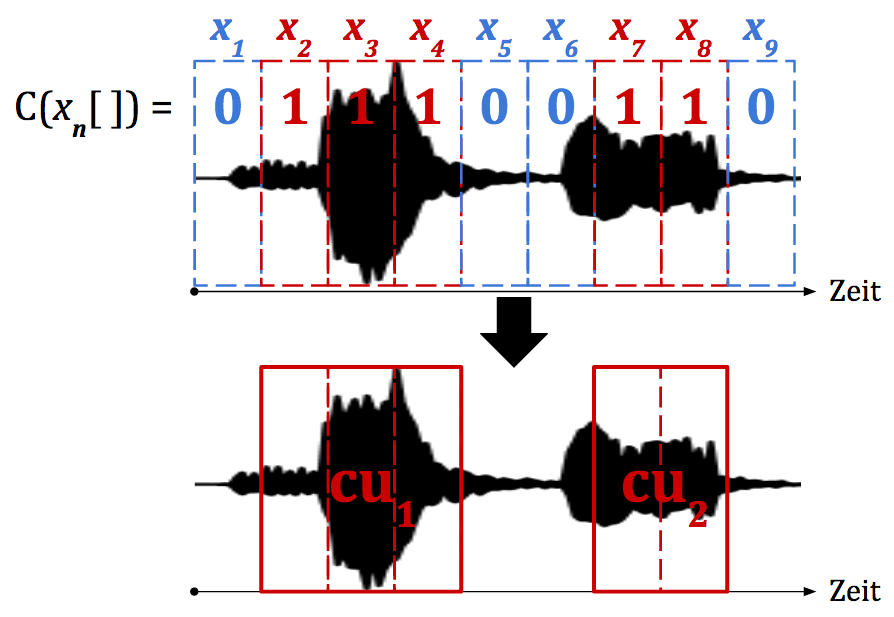
\includegraphics[width=0.6\textwidth]{bilder/cry-Unit02.png}
	\caption{Zusammenfassung der als stimmhaft klassifizierter Signalfenster zu Schreieinheiten}
	\label{img:cryUnit}
\end{figure}

\autoref{eq:cry-Unit} definiert den Datentyp \textbf{Schreieinheit} (engl. \emph{Cry-Unit}) [$CU$]. Eine Schreieinheit wird bestimmt durch einen Anfangszeitpunkt $start$, einen Endzeitpunkt $end$ und der Liste ihrer Signalfenster $windows = \big[x_0[\;], \ldots, x_n[\;]\big]$.

\begin{equation}
CU := \quad \Big(windows = \big[x_0[\;] \; ,\ldots, x_n[\;] \big] \;, start \in Zeit \;, end \in Zeit \Big)
\label{eq:cry-Unit}
\end{equation}

Die zeitliche Dauer eine Schreieinheit $cu \in CU$ wird nach \autoref{eq:cry-Lambda} berechnet und mit $\lambda$ bezeichnet. Die Dauer der Pause zwischen zwei Schreieinheiten d($cu_i, cu_j$), wird nach \autoref{eq:cry-distance} berechnet. Diese Zusammenhänge werden in \autoref{img:cryUnit-details} visualisiert.\cite[S. 2]{vad_entropy}

\begin{equation}
\lambda (cu) = cu.end - cu.start
\label{eq:cry-Lambda}
\end{equation}

\begin{equation}
\text{d}(cu_i, cu_j) = cu_j.start - cu_i.end
\label{eq:cry-distance}
\end{equation}

\begin{figure}[h]
	\centering
	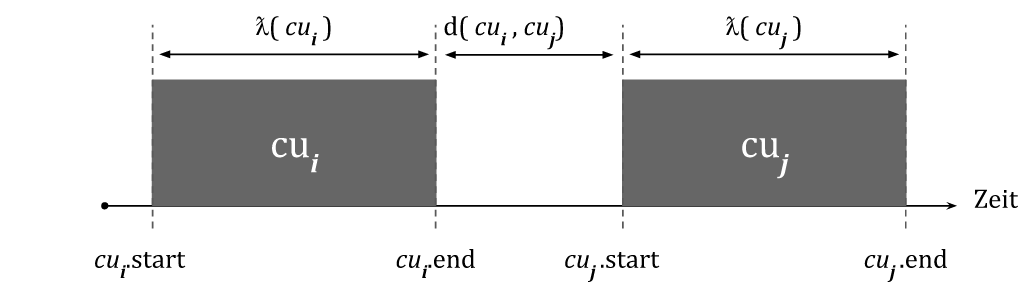
\includegraphics[width=0.95\textwidth]{bilder/newSmoothing05.png}
	\caption[Beziehungen zwischen benachbarten Schreieinheiten]{Beziehungen zwischen benachbarten Schreieinheiten (nach \cite[S. 2]{vad_entropy})}
	\label{img:cryUnit-details}
\end{figure}

Algorithmus \autoref{alg:cryUnit} zeigt in Pseudo-Code, wie in einem Eingangssignal $x[\;]$ die Schreieinheiten gekennzeichnet werden. Der Output des Algorithmus ist eine Liste aller im Signal detektierten Schreieinheiten $CU_{all} = [cu_0 , \ldots, cu_l]$. Die Funktion \textsc{turnSignalIntoOverlappingWindows} ($x[\;], length, hopsize$) zerlegt das Eingangssignal in einander überlappende Signalfenster. Wie in Unterabschnitt \ref{sec:windowing} beschrieben, wurde  $length = \SI{25}{\milli\second}$ und $hopsize = \SI{12.5}{\milli\second}$ festgelegt. Der Output dieser Funktion ist eine Liste aller Signalfenster $X_{all} = [x_0[\;] ,\ldots, x_m[\;]]$. Die Funktion $C(x_i[\;])$ ist diejenige, die im Zuge der Simulationsstudie der VAD festgelegt wurde und klassifiziert ein Signalfenster als \emph{Stimme} oder \emph{Sille} nach \autoref{eq:cepTree01}. Die Funktion \textsc{getTimeOf}$(x_i[\;])$ liefert den Anfangszeitpunkt des Signalfensters $x_i[\;]$. 

\begin{algorithm}[h]
	\caption{Detektion Schreieinheiten in einem Audiosignal}
	\label{alg:cryUnit}
	\begin{algorithmic}[1]
		\Function{DetectCryUnitsInSignal}{$x[\;], hopsize, overlap$}
		\State $X_{all} = $ \Call{turnSignalIntoOverlappingWindows}{$x[\;], hopsize, overlap$}
		\State $ CU_{all} \gets [\;]$
		\State $ cu\gets ([\;],0,0)$
		\For{\textbf{all} $x_i[\;] \in X_{all}$}
				\State $ c \gets C(x_i[\;])$
				\State \Comment Start of Cry-Unit
				\If {$c == 1 \wedge $ \Call{isEmpty}{cu.windows}}
						\State $cu\gets ([\;],0,0)$
						\State $cu.start \gets $ \Call{getTimeOf}{$x_i[\;]$}
						\State $cu.windows \gets [cu.windows, x_i[\;]]$
				\EndIf
				\State \Comment Inside Cry-Unit
				\If {$c == 1 \wedge $ \Call{isEmpty}{cu.windows}}
						\State $cu.windows \gets [cu.windows, x_i[\;]]$
				\EndIf
				\State \Comment End of Cry-Unit
				\If {$c == 0 \wedge $ ! \Call{isEmpty}{$cu.windows$}}
						\State $cu.end \gets $ \Call{getTimeOf}{$x_i[\;]$}
						\State $CU_{all} \gets [CU_{all}, cu]$
						\State $cu.windows \gets [\;]$
				\EndIf
		\EndFor
		
		%\State \Comment End last Cry-Unit by force if still open.
		%\If {$\text{ ! isEmpty}(cu.windows) == 0$}
		%\State $cu.end \gets  getTimeOf(X_{windows}[end])$
		%\State $CU_{all} \gets [CU_{all}, cu]$
		%\EndIf
		
		\Return $CU_{all}$
		
		\EndFunction
		
	\end{algorithmic}
\end{algorithm}


\section{Nachträgliche Korrektur von Schreieinheiten}
\label{sec:decision_smoothing_new}

\autoref{img:beforeSmoothing} zeigt ein Audiosignal mit einem Signal-Rausch-Abstand von \SI{5}{\decibel}, bei dem die Voice Activity Detection durchgeführt wurde. Die rote Linie zeigt die tatsächliche Klassifizierung und die grüne Linie die prognostizierte Klassifizierung. Es ist zu sehen, dass einige False-Negatives sowie False-Positives prognostiziert wurden. Es werden drei charakteristische Varianten falsch prognostizierter Klassifizierungen näher erläutert:

\begin{description}
	\item [False Negatives nach (a): ] Eine korrekt erkannte, längere Schreieinheit wird zu früh beendet. Oft werden kurz nach dem Ende einer längeren Schreieinheit sehr kurze Schreieinheiten prognostiziert, die eigentlich noch zu der längeren, vorhergehenden Schreieinheit gehören.
	\item [False Positives nach (b): ] Kurze Schreieinheiten werden in eigentlichen Stille-Bereichen erkannt.
	\item [False Negatives nach (c): ] Eine Schreieinheit zerfällt in zwei kürzere Schreieinheiten, da einige wenige Signalfenster in der Mitte als Stille erkannt wurden.
\end{description}

\begin{figure}[h]
	\centering
	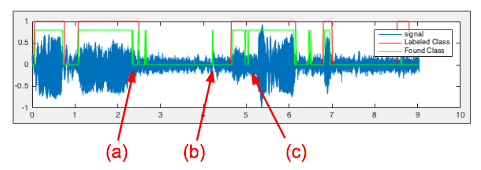
\includegraphics[width=0.8\textwidth]{bilder/smoothing02.png}
	\caption[Klassifizierung vor dem Decision-Smoothing]{Klassifizierung vor dem Decision-Smoothing}
	\label{img:beforeSmoothing}
\end{figure}

Im Process des \emph{Decision-Smoothing} werden kontextuelle Informationen genutzt, um nachträglich False-Positives und False-Negatives zu entfernen. Dazu werden die von Waheed et al. \cite{vad_entropy} präsentierten Ideen verwendet. Es werden zwei Parameter eingeführt: $\lambda_{min}$, die Mindestlänge einer akzeptierten Schreieinheit, und d$_{min}$, die Mindestlänge einer akzeptierten Pause zwischen Schreieinheiten. Das Decision-Smoothing wird nach den folgenden Entscheidungsregeln durchgeführt:

\textbf{Entscheidungsregeln: }\noindent\rule{0.7\linewidth}{0.3pt}
\begin{itemize}
	\item ist $\lambda (cu_{i}) \leq \lambda_{min}$ ?
	\begin{itemize}
		\item wenn $\lambda (cu_{i-1}) > \lambda_{min}$ und $d (cu_{i-1}, cu_{i}) \leq d_{min}$, dann vereinige $cu_{i}$ mit $cu_{i-1}$ $\Longrightarrow$ behebt False-Negatives des Types (a)
		\item ansonsten entferne $cu_i \Longrightarrow$ behebt False-Negatives des Types (b)
	\end{itemize}
	\item wenn $\lambda (cu_{i}) > \lambda_{min}$ und $d (cu_{i-1}, cu_{i}) \leq d_{min}$, dann vereinige $cu_{i}$ mit $cu_{i-1}$ . $\Longrightarrow$ behebt False-Negatives des Types (c)
\end{itemize}
\noindent\rule{\linewidth}{0.3pt}

Die Entscheidungsregeln greifen nur auf die letzten beiden erkannten Schreieinheiten zu, um eine kontinuierliche Analyse zu gewährleisten. Bei einer Offline-Analyse können die Entscheidungsregeln vereinfacht werden, da die False-Negatives nach Typ (a) und (c) mit der selben Regel abgefragt werden können. Algorithmus \autoref{alg:decisionSmoothing} zeigt in Pseudo-Code, wie das Decision-Smoothing durchgeführt wird. Input des Algorithmus ist eine Liste mit Schreieinheiten $CU_{all} = [cu_0 , \ldots , cu_l]$, die durch Algorithmus \ref{alg:cryUnit} entstanden ist, sowie die Grenzwerte $\lambda_{min}$ und $d_{min}$. Die Indexierung der Liste $CU_{all}$ beginnt bei 0. Der Output der Funktion ist eine Liste aller im Signal enthaltenenen Schreieinheiten $CU_{smoothed}$ mit korrigierten Anfangs- und Endzeitpunkten.
 
In verschiedenen Veröffentlichungen wurden unterschiedliche Mindestlängen von Schreieinheiten festgestellt. Várallyay \cite[S. 8]{cry_thesis} hat beispielsweise eine Mindestlänge von \SI{250}{\milli\second} gemessen. Der niedrigste Wert, der nach dem Wissen des Autors in einer Veröffentlichung genannt wurde, stammt von Zeskind et al. \cite[S. 325]{rythmic} und beträgt  \SI{60}{\milli\second}. Dieser Wert wurde für $\lambda_{min}$ in dieser Arbeit übernommen. Es konnten hingegen keine Veröffentlichungen gefunden werden, bei denen die geringste Pausenlänge gemessen wurde. Der Wert wurde ebenfalls mit $d_{min} = \SI{60}{\milli\second}$ bestimmt. \autoref{img:after-smoothing} zeigt das Beispielsignal vor und nach dem Decision-Smoothing. 

\begin{figure}[h]
	\centering
	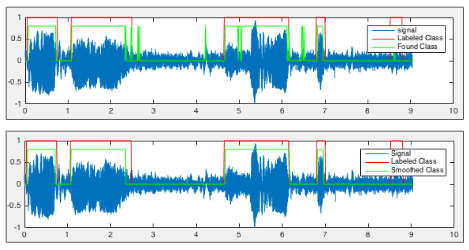
\includegraphics[width=0.8\textwidth]{bilder/smoothing04.png}
	\caption[Klassifizierung nach dem Decision-Smoothing]{Oben: Prognostizierte Klassifizierung vor dem Decision-Smoothing. Unten: Prognostizierte Klassifikation nach dem Decision-Smoothing.}
	\label{img:after-smoothing}
\end{figure}

\begin{algorithm}[h]
	\caption{Nachträgliche Korrektur von Schreieinheiten}
	\label{alg:decisionSmoothing}
	\begin{algorithmic}[1]
		\Function{decision-Smoothing}{$CU_{all}, \lambda_{min}, d_{min}$}
		\State $CU_{smoothed} \gets[CU_{all}[0]] $
		\State \Comment start for-loop at the \emph{second} cry-Unit!
		\For{ $i = 1 , \ldots ,$ \Call{length}{$CU_{all}$} - 1}
			\State $cu_i \gets CU_{all}[i]$
			\State $cu_{i-1} \gets CU_{smoothed}[end]$
			\If{$\lambda(cu_i) > \lambda_{min}$}
			\State \Comment Accept Cry-Unit
			\If{d$(cu_{i-1},cu_{i}) > d_{min}$}
					\State $CU_{smoothed} \gets [CU_{smoothed}, cu_i] $
			\Else
					\State \Comment Erase False-Negative of Type (c)
					\State $cu_i \gets $ \Call{vereinige}{$cu_i, cu_{i-1}$}
					\State $CU_{smoothed} \gets [CU_{smoothed}[1:end-1], cu_i] $
			\EndIf
			\Else
			\State \Comment Erase False-Negative of Type (a)
			\If{$d(cu_{i-1},cu_{i}) \leq d_{min}$ }
			\State $cu_i \gets $ \Call{vereinige}{$cu_i, cu_{i-1}$}
			\State $CU_{smoothed} \gets [CU_{smoothed}[0:end-1], cu_i] $
			\Else
			\State \Comment Don't accept $cu_i$. Erases False-Positives of Type (b)
			\EndIf
			\EndIf
		\EndFor
		
		\Return $CU_{smoothed}$
		\EndFunction
		
	\end{algorithmic}
\end{algorithm}





\chapter{Ableitung der Schmerz Score}
\label{sec:deduction}

In Kapitel \ref{sec:marking_cry-units_new} wurden Methoden vorgestellt, durch die einem Audiosignal die Cry-Units erkannt und markiert werden. Diese Cry-Units bilden den Ausgangspunkt, um eine Schmerz Score ableiten zu können. 

Wie in Kapitel \ref{sec:painScores} erläutert wurde, wird eine Schmerz Score typischerweise nicht aus den Informationen einer einzelnen Cry-Unit, sondern aus Gruppen mehrerer Cry-Units innerhalb eines längeren Beobachtungszeitraumes geschlossen. Dafür ist es zunächst notwendig, diejenigen Cry-Units zu identifizieren, die gemeinsam einem schmerzversuchanden Stimulus zugeordnet werden können. Diese Gruppierung von Cry-Units wird in dieser Arbeit als \emph{Segmentierung} bezeichnet und in Kapitel \ref{sec:segmenting} vorgestellt. Die so entstandenen Segmente bilden die Basis zur Ableitung von Schmerz Scores, welche in Kapitel \ref{sec:marking_cry-units_new} diskutiert wird.


\section{Segmentierung}
\label{sec:segmenting}

Wie in Kapitel \ref{sec:painScores} erläutert wurde, wird die Schmerzdiagnose für Post-Operativen Schmerz mit Pain Scales typischerweise umgesetzt, indem das Baby in bestimmten Intervallen besucht und für einen festgelegten Zeitraum beobachtet wird, worauf den Schmerzgrad für einen bestimmten Zeitpunkt diagnostiziert wird. So empfiehlt die Pain Scale PAT, das Baby alle 30 Minuten zu besuchen und für 15 bis 30 Sekunden zu beobachten. Für viele Pain Scales konnten diese  Beobachtungsintervalle und Zeiträume nicht in Erfahrung gebracht werden. 

Dieses Vorgehen der Schmerzdiagnose nur zu festgelegten Zeitintervallen macht keinen Sinn für ein kontinuierliches System, da es den Vorteil der Kontinuierlichkeit eliminieren würde. Die Frage ist also, wann eine medizinische Fachkraft den Anfangszeitpunkt einer Schmerzdiagnose festlegen würde, würde es das entsprechende Baby rund um die Uhr beobachten, und nicht nur eine Visite zu festgelegten Zeitpunkten durchführen. Die logisch nächstliegende Antwort ist, die Schmerzdiagnose genau dann zu starten, wenn das Baby anfängt, zu schreien. 

Die nächste Frage ist, wann man die Beobachtung wieder beendet und eine Schmerz Score für den beobachteten Zeitraum festlegt. Da einige Pain Scales aus Tabelle \ref{tab:painscores} Beobachtungszeiträume angeben, kann argumentiert werden, dass die Beobachtung direkt nach dem für die jeweilige Scale angegebenen Zeitraum beendet werden und eine Pain Score abgeleitet werden kann, auch, wenn das Baby weiterhin schreit. Dabei stellt sich die Frage, welche Zeiträume man für die Pain Scales festlegt, die keinen selber keinen vorschreiben. Die zweite Frage ist, ob eine Vorzeitige Beendigung der Beobachtung überhaupt sinnvoll ist, wenn ein automatisierte System zur Verfügung steht und der Beobachter somit \glqq unendlich viel Zeit hat\grqq . Daher wird an dieser Stelle zuerst die grundlegendere Frage gestellt: Was ist der längste sinnvolle Zeitraum, für den eine Pain Score abgeleitet werden kann? Die nächstliegende Antwort ist: Dann, wenn das Kind aufhört, zu schreien.

Auf Basis dieser Argumentation wurde das folgende Vorgehen zur kontinuierlichen Segmentierung entwickelt: Wenn das Baby keine Äußerungen von sich gibt, weil es beispielsweise schläft, wird keine Cry-Unit festgestellt, und somit existiert auch momentan kein offenes Segment. Fängt das Baby an, einen Laut von sich zu geben, also eine Cry-Unit zu produzieren, wird ein neues Segment eröffnet und die Cry-Unit diesem Segment hinzugefügt. Weitere Cry-Units werden so lange diesem Segment hinzugefügt, wie die Dauer der Stille nach einer Cry-Unit einen festgelegten Grenzwert $t_{s}$ nicht überschreitet. Ein Cry-Segment wird dann geschlossen, wenn das Baby für einen festgelegten Zeitraum keine Laute mehr von sich gibt, also \glqq aufhört, zu weinen\grqq{}. Das Endzeitpunkt des Segmentes wird als der Endzeitpunkt der letzten Cry-Unit des Segmentes festgelegt.

Formel \ref{eq:cry-segment}  definiert ein \emph{Cry-Segment} [$CS$] als Datentyp. Ein Cry-Segment ist eine Liste von Cry-Units. Alle Cry-Units erfüllen die Nebenbedingung \ref{eq:cry-segment-nb}, das heißt, dass die Distanzen aller benachbarter Cry-Units eines Cry-Segments unterhalb des Grenzwertes $t_{s}$ liegen.

\begin{equation}
CS = [cu_0 ,  \ldots,  cu_n]
\label{eq:cry-segment}
\end{equation}

\begin{equation}
\forall cs \in CS: \forall i = 0 \ldots length(cs)-2 : d(cs[i], cs[i+1]) < t_{s}
\label{eq:cry-segment-nb}
\end{equation}

Der Start-Zeitpunkt eines Cry-Segments wird nach Formel \ref{eq:cry-segment-start} als der Startzeitpunkt der ersten Cry-Unit des Segments definiert. Das Ende eines Segmentes wird definiert als der Endzeitpunkt der letzten Cry-Unit nach Gleichung \ref{eq:cry-segment-end}.

\begin{equation}
start(cs) = cs[0].start
\label{eq:cry-segment-start}
\end{equation}

\begin{equation}
end(cs) = cs[n].end
\label{eq:cry-segment-end}
\end{equation}

Algorithmus \ref{alg:crySegment} zeigt einen Pseudocode, wie die Segmentierung nach dem beschriebenen Prinzipien offline durchgeführt wird. Input des Algorithmus ist die Liste aller Cry-Units $CU_{all} = [cu_0 ,\ldots, cu_m]$, die durch das Decision-Smoothing nach Algorithmus \ref{alg:decisionSmoothing} entstanden ist. Das Ergebnis des Algorithmus ist die Liste $CS_{all}$, die alle gefundene Cry-Segmente  $[cs_0 , \ldots ,  cs_n]$ enthält. Der Algorithmus eignet sich nicht für eine Online-Segmentierung, da das Ende eines Segmentes erst bei Beginn eines neuen Segmentes festgestellt wird, wobei beliebig viel Zeit zwischen den Beiden Segmenten liegen kann. Wurde beispielsweise $t_{s} = \SI{1}{\minute}$ festgelegt, und die Pause zwischen zwei Segmenten beträgt eine Stunden, so wäre das Ende des ersten Segmentes 59 Minuten zu spät festgestellt worden. Bei einer online durchgeführten Segmentierung empfiehlt es sich, die Dauer der Stelle nach jeder neu erkannten Cry-Unit kontinuierlich zu Messen und ein Segment sofort zu beenden, wenn ein Stillezeitraum den Grenzwert $t_s$ überschreitet.

\begin{algorithm}[h]
	\caption{Gruppierung von Cry-Units zu Cry-Segments}
	\label{alg:crySegment}
	\begin{algorithmic}[1]
		\Function{segmentCryUnits}{$CU_{all}, t_{s}$}
		\State $ CS_{all} \gets [\;]$
		\State $ cs \gets [CU_{all}[0]]$
				\For{ $i = 1 , \ldots , length(CU_{all}) - 1$}
						\State $ cu_i \gets CU_{all}[i]$
						\State $cu_{i-1} \gets CU_{all}[i-1]$
						\If{d$(cu_{i-1},cu_i) < t_{seg-max}$}
								\State $cs \gets [cs_i , cu_i]$
						\Else
								\State $CS_{all} \gets [CS_{all}, cs]$
								\State $cs \gets [cu_i]$
						\EndIf
				\EndFor
		\Return $CS_{all}$
		
		\EndFunction
		
	\end{algorithmic}
\end{algorithm}

Abbildung \ref{img:segmenting06} zeigt die nach dieser Methode durchgeführte Segmentierung anhand eines Beispiels.

Das hier vorgestellte Vorgehen wurde absichtlich möglichst einfach gehalten, damit der Sinn des Parameters $t_{s}$ leicht ersichtlich ist und somit von der medizinischen Fachkraft selbständig festgelegt werden kann. Schlussendlich ist eines der Hauptziele dieser Segmentierung, unnötige Berechnungen von Schmerz-Scores in den nachfolgenden Schritten zu vermeiden, so lange keine Cry-Units vorliegen. Das Ende eines Segmentes ist außerdem ein günstiger Zeitpunkt, um die Parameter des Kompressors im Pre-Processing auf Basis des RMS-Wertes des Segmentes zu aktualisieren (siehe Kapitel \ref{sec:preprocessing}). Trotz der Trivialität dieser laufenden Segmentierung liegt hier ein wichtiger Unterschied im Gegensatz zu vergleichbaren Systemen, wie zum Beispiel das von Cohen et al. \cite{cohenCry}, bei dem die Entscheidung über Cry/not-Cry für Segmente mit einer festen Fenstergröße von 10 Sekunden vorgenommen wird. 

\begin{figure}[H]
	\centering
	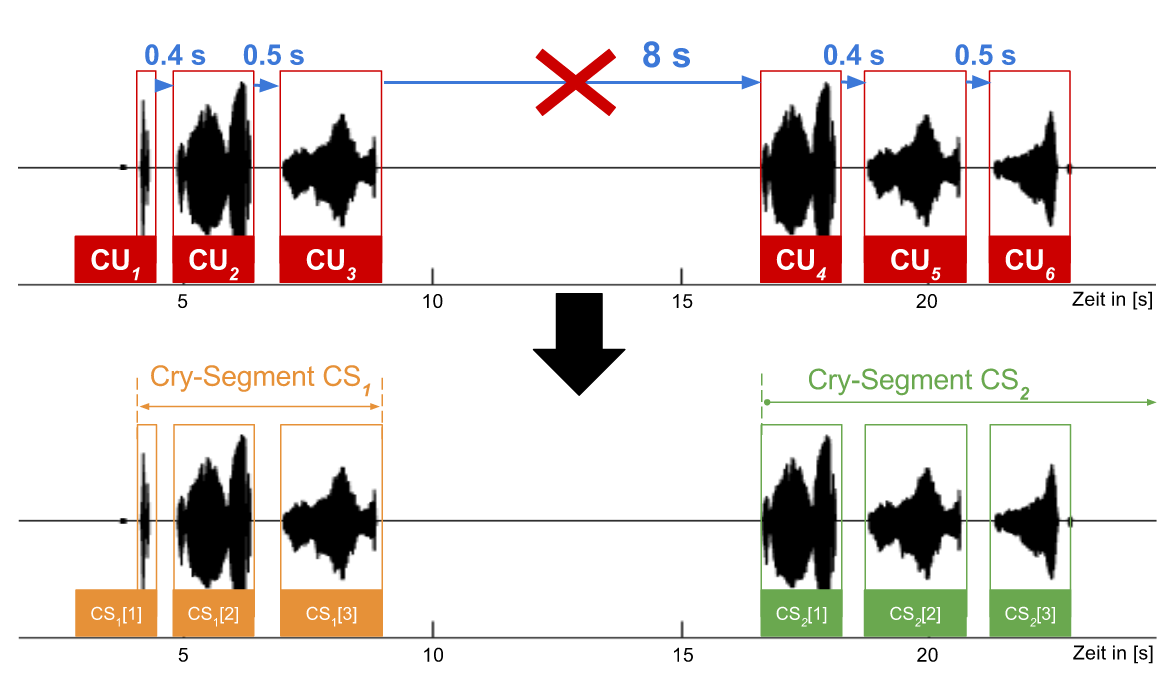
\includegraphics[width=1\textwidth]{bilder/segmentierung06.png}
	\caption{Beispiel für eine Segmentierung mit einem Grenzwert von $t_s = \SI{6}{\second}$}
	\label{img:segmenting06}
\end{figure}

\section{Extrahierung von Eigenschaften und Ableitung der Schmerzscore}
\label{sec:overviewPainRegression}

Das Ergebnis der Segmentierung ist eine Liste an Cry-Segmenten $cs_0,  \ldots , c_n$. Diese Cry-Segmente bilden nun die Basis für die Ableitung der Pain Score. Die medizinische Fachkraft, die das System verwendet, muss dabei zuerst die Wahl treffen, welche Pain Scale verwendet werden soll. Das einfachste denkbare Vorgehen ist die Ableitung genau einer Pain Score aus den globalen Eigenschaften eines Segmentes, wobei diese Ableitung erst vollzogen werden kann, sobald ein Segment abgeschlossen wurde und alle Informationen für dieses Segment vorliegen. Es wird also jedem Segment genau eine Pain Score zugewiesen. Das Vorgehen wird am Beispiel der NIPS aus Tabelle \ref{tab:nips} verdeutlicht: Dabei steht die Abwesenheit von Weinen für null Punkte, \glqq mumbling\grqq{} (murmeln) für einen Punkt und \glqq vigorous\grqq{} (energisch) für zwei Punkte. Bei Abwesenheit von Lautäußerungen, also der Zeitraum zwischen den Segmenten, werden also keine Punkte = null Punkte vergeben. Ein Segment, dessen Qualität insgesamt als \glqq murmelnd\grqq{} bewertet wird, erhält einen Punkt, und ein Segment, welches als insgesamt als \glqq energisch\grqq{} bewertet wird, zwei Punkte. Das Problem ist offensichtlich: \glqq murmelnd\grqq{} und \glqq energisch\grqq{} sind subjektiv behaftete Begriffe und lassen sich nicht ohne weiteres aus den Eigenschaften eines Segmentes feststellen. 

Es werden zwei verschiedene Lösungs-Strategien für dieses Problem vorgestellt. 

\vspace{5mm}

\textbf{Strategie 1} \noindent\rule{0.83\linewidth}{0.3pt}\\
... löst das Problem mit Hilfe von \emph{Regression} (Siehe Kapitel \ref{sec:regression}):
\begin{enumerate}
 \item Man erstellt eine Datenbank mit Aufnahmen von kindlichen Lautäußerungen, die man segmentiert.
 \item Man errechnet \glqq so viele \emph{objektiv} messabare Eigenschaften wie möglich\grqq{} für jedes Segment, wie zum Beispiel die insgesamte Länge, die durchschnittliche Länge der enthaltenen Cry-Units, durchschnittliche Tonhöhe usw.
 \item Man bittet medizinische Fachkräfte, für jedes Segment der Datenbank eine Score bezüglich einer Pain Scale zu vergeben. Dadurch erhält man eine gelabelte Test-Datenbank.
 \item Man verwendet einen \emph{Regressionsalgorithmus}, um den Zusammenhang zwischen den in Schritt 2 objektiv gemessenen Eigenschaften der Segmente und den in Schritt 3 vergebenen \emph{Scores} herzustellen. An dieser Stelle kann zum Beispiel die in Kapitel \ref{sec:multipleRegression} beschriebene multiple lineare Regression verwendet werden. Man erhält somit einen Regressor für jede Pain Scale.
 \item Möchte man für neue, unbekannte Segmente die Pain Score prognostizieren, nutzt man den entsprechenden Regressor.
\end{enumerate}
\noindent\rule{\linewidth}{0.3pt}

Das Vorteil dieses Vorgehens ist, dass das Problem der Übersetzung der objektiv messbaren Parameter in die subjektiv behafteten Begriffe überbrückt wird, indem die Regression direkt von den objektiv messbaren Parametern auf  die Pain Score durchgeführt wird. Der Nachteil ist, dass eine Testdatenbank für jede Pain Scale aufgebaut werden muss. Wird ein neue Pain Scale eingeführt, muss der Regressor für diese Scale durch erneutes Labeln festgestellt werden. Ein weiterer Effekt der Abbildung des Problems als Regression ist, dass ein Regressor in einen kontinuierlichen Zahlenraum abbildet. Es sind also Regressionsergebnisse wie zum Beispiel $2.8$ denkbar. Diese \glqq bessere Auflösung\grqq{} kann als Vorteil betrachtet werden. Ist jedoch eine direkte Übersetzung der Pain Scale inklusive der ganzzahligen Punktzahlen gewünscht, so stellt sich die Frage, ob eine $2.8$ auf- oder abzurunden ist.

\vspace{5mm}

\textbf{Strategie 2} \noindent\rule{0.83\linewidth}{0.3pt} \\
... löst das Problem mit Hilfe von Klassifizierung (Siehe Kapitel \ref{sec:classification}):
\begin{enumerate}
	\item und 2. entsprechen Strategie 1
	\stepcounter{enumi}
	\item Man sammelt alle subjektiven Begriffe, die in Pain Scales verwendet werden, wie zum Beispiel \glqq murmelnd\grqq , \glqq energisch\grqq , usw.
	\item Man bittet medizinische Fachkräfte, jedes Segment der Datenbank mit denjenigen Begriffen zu labeln, die die jeweilige Person für zutreffend hält. 
	\item  Man Verwendet einen \emph{Klassifizierungsgorithmus}, um einen Zusammenhang zwischen den in Schritt 2 festgestellten objektiv messbaren Eigenschaften der Segmente und den \emph{subjektiv behafteten Begriffen} zu finden. Man erhält somit einen Klassifikator für jeden Begriff, der binär in \emph{positive = zutreffend} und \emph{negative = nicht zutreffend} klassifiziert.
	\item Möchte man für neue, unbekannte Segmente die Pain Score prognostizieren, so wird für jede mögliche Score der Pain Scale überprüft, ob für alle subjektiv beschreibenden Begriffe der entsprechende Klassifikator ein positive prognostiziert. Die Ableitung der Score ist somit ein weiters Klassifizierungsproblem, wobei eine Score einer Klasse entspricht und genau dann abgeleitet werden kann, wenn alle Vorraussetzungen für die Klasse erfüllt sind.
\end{enumerate}
\noindent\rule{\linewidth}{0.3pt}

Der Vorteil dieser Methode ist, dass auch zum Zeitpunkt der Erstellung der Testdatenbank unbekannte Pain Scales zu einem späteren Zeitpunkt eingebunden werden können, insofern alle in dieser neuen Pain Scale verwendeten subjektiv behafteten Begriffe bereits gelabelt vorliegen, weil sie auch in anderen Pain Scales verwendet wurden. Das Vorgehen erlaubt somit eine gewissen Flexibilität bezüglich zukünftig entwickelter Pain Scales. Der Nachteil dieser Methode ist, dass durch die Umwandlung der eigentlich quantitativ geordenten Score einer Pain Scale in qualitative Klassen aus einem implizit als Regression zu betrachtenden Problem ein Klassifizierungsproblem macht. Dies wirft neue Fragen auf, wie zum Beispiel: Angenommen, bei einer fiktiven Pain Scale wird jede Score mit jeweils drei subjektiv behafteten Begriffen beschrieben, und bei der Klassifizierung eines Segmentes wird festgestellt, dass für jede Punktzahl genau zwei der drei Begriffe erfüllt werden. Welche Score wird dann prognostiziert? Ein anderes Beispiel wird am Beispiel der der NIPS-Score aus Tabelle \ref{tab:nips} verdeutlicht: Angenommen, ein Cry-Segment enthält hörbar \glqq starkes\grqq{} Schreien, es kann jedoch weder \glqq mumbling (murmelnd) \grqq{} noch \glqq vigorous (energisch)\grqq{} abgeleitet werden. Demzufolgen müsste dieses Segment eine Score von 0 Punkten erhalten, wobei ein Mensch in dieser Situation eventuell \glqq stark\grqq{} zu \glqq heftig\grqq{} uminterpretieren und 2 Punkte vergeben hätte. Strategie 1 ist weniger anfällig für dieses Problem.

In jedem Fall werden medizinische Fachkräfte benötigt, um das Labeling der Cry-Segmente durchzuführen, was aus Zeitgründen im Rahmen dieser Arbeit nicht möglich ist. Die Aquise von Audioaufnahmen von Babys sowie das Labeling der Aufanhmen erfodern nicht nur Zeit, sondern das Fachwissen über das Führen und die Auswerten von Interviews.

\subsection{Extrahierung von Eigenschaften}
\label{sec:segmentFeatures}

Im vergangenen Kapitel wurde erläutert, dass die Basis für die Ableitung einer Pain Score für ein Segment die Extraktion von \glqq so vielen Features wie möglich\grqq{} ist. In diesem Kapitel wird präzisiert, welche Features gemeint sind.  Varallyay \cite[S. 16 - 17]{cry_thesis} schlug vor, drei Kategorien an Features zu betrachten: 1.) Features des Zeitbereichs, 2.) Features der Frequenzbereichs, und 3.) Melodie-bezogene Attribute. Diese Kategorisierung wurde für diese Arbeit übernommen.

In Kapitel \ref{sec:acousticModel} wurde beschrieben, welche Features in der medizinischen Schreiforschung typischerweise extrahiert wurden. In Kapitel \ref{sec:cryDiscussion} wurde diskutiert, dass 1.) nicht bewiesen ist, welche Features die \glqq wichtigsten\grqq{} sind und 2.) keine Einigung darüber herrscht, wie genau bestimmte Features zu berechnen sind. Basierend auf den in diesem Kapitel vorgestellten Features werden in diesem Kapitel konkrete Berechnungsvorschriften definiert. Welche von diesen Features tatsächlich im Zusammenhang mit Schmerz stehen, lässt sich erst in der anschließenden Nutzung der Features zur Regression oder Klassifizierung der Pain Scales feststellen, welche jedoch im Rahmen dieser Arbeit nicht durchgeführt werden kann.

\subsubsection{Features des Zeitbereiches}

Mit Features des Zeitbereiches sind solche gemeint, die sich allein aus Kenntnis der der Start- und Endzeitpunkte der im Segment enthaltenen Cry Units sowie deren Zeitbereiche gewinnen lassen, wie beispielsweise die durchschnittliche Länge der Cry-Units oder die durchschnittliche Energie der Cry-Units. In diesem Kapitel gilt die Konvention, dass eine Cry-Segment $cs$ insgesamt $N$ Cry-Units enthält, die Indexierung wird mit $0 \ldots N-1$ definiert.

\begin{description}
\item[Segment-Length: ] Zeitliche Länge des Segmentes:
\begin{equation}
\text{Segment-Length}(cs) = cs[N-1].end - cs[0].start
\label{eq:segment_length}
\end{equation}

\item[Density: ] Relativer Anteil der Cry-Units an der Länge des Segmentes (\glqq Dichte\grqq{})
\begin{equation}
\text{Density}(cs) = \frac{\sum_{i = 0}^{N-1} \lambda(cs[i])}{\text{Segment-Length}(cs)}
\end{equation}

\item[Tempo:] Das Verhältnis zwischen der Dauer des Segmentes und der Anzahl der Cry-Units. Dieses Feature ähnelt dem von LaGasse et al. \cite[S. 85]{parentalPerception} als \emph{Utterances} bezeichneten Feature.

\begin{equation}
\text{Tempo}(cs) =  \frac{N}{\text{Segment-Length}(cs)}
\end{equation}

\item[Statistics of Cry-Units:] Statistische Auswertungen bezüglich der \emph{Länge der Cry-Units} $\text{stats}_{cu}(cs)$: Durchschnitt, Median, Minimum, Maximum und Standardabweichung der Cry-Units. Das $\text{mean}_{cu}(cs)$-Feature wird von LaGasse et al. \cite[S. 85]{parentalPerception} und vielen weiteren Schreiforschern als \emph{Mean Duration} bezeichnet.

\begin{equation}
\text{stats}_{cu}(cs) = 
\begin{dcases}
\text{mean}_{cu}(cs) = \meani_{i = 0 \ldots N-1}\{\lambda(cs[i])\} \\
\text{median}_{cu}(cs) = \mediani_{i = 0 \ldots N-1}\{\lambda(cs[i])\} \\
\text{min}_{cu}(cs) = \mini_{i = 0 \ldots N-1}\{\lambda(cs[i])\} \\
\text{max}_{cu}(cs) = \maxi_{i = 0 \ldots N-1}\{\lambda(cs[i])\} \\
\sigma_{cu}(cs) =  \sigma_{i = 0 \ldots N-1}\{\lambda(cs[i])\} 
\end{dcases}
\label{eq:featuresOfCryUnits}
\end{equation}

\item[Statistics of Bursts:]\footnote{Erläuterung zum Begriff \emph{Burst} in Kapitel \ref{sec:acousticModel}} Die in Gleichung \ref{eq:featuresOfCryUnits} definierten Features können ebenso in Bezug auf die \emph{Längen der Bursts} errechnet werden, in dem in jeder Gleichung $\lambda(cs[i])$ ersetzt wird durch $cs[i].start - cs[i-1].start$. Die Indexierung muss auf $i = 1 ,\ldots, N-1$ begrenzt werden.

\begin{equation}
\text{stats}_{burst}(cs) = 
\begin{dcases}
\text{mean}_{burst}(cs) = \meani_{i = 1 \ldots N-1}\{cs[i].start - cs[i-1].start\} \\
\text{median}_{burst}(cs) = \mediani_{i = 1 \ldots N-1}\{cs[i].start - cs[i-1].start\} \\
\ldots
\end{dcases}
\label{eq:featuresOfBursts}
\end{equation}

\item[Statistics of Pauses:] Nach dem selben Muster werden die statistischen Auswertungen bezüglich der  \emph{Längen der Pausen} ermittelt. Eine Pause entspricht in diesem Zusammenhang der Distanz zwischen zwei auf einander folgenden Cry-Units nach Gleichung \ref{eq:cry-distance}.

\begin{equation}
\text{stats}_{pause}(cs) = 
\begin{dcases}
\text{mean}_{pause}(cs) = \meani_{i = 1 \ldots N-1}\{d(cs[i-1],cs[i])\} \\
\text{median}_{pause}(cs)  = \ldots
\end{dcases}
\end{equation}

\item[Statistics of Energies:] Zunächst wird die Liste aller in den Cry-Units enthaltenen Signalfenster definiert nach Gleichung \ref{eq:windowsOfSegment}. Eine Cry-Unit hat die Signalfenster $cu.windows = x_0[\;],\ldots,x_m[\;]$

\begin{equation}
x_{seg}[\; ] = cs[0].windows[0] \;  , \; \ldots \; , \; cs[N-1].windows[m] 
\label{eq:windowsOfSegment}
\end{equation}

Die Liste $x_{seg}[\; ]$ hat $R$ Elemente, die Indexierung wird definiert mit $0, \ldots, R-1$. Gleichung \ref{eq:energyStats} definiert die Features bezüglich der MSV-Werte (\glqq Lautstärken\grqq ) des Segmentes. Der MSV-Wert als Maß des durchschnittlichen Energiegehaltes wurde in Gleichung \ref{eq:msv} definiert.

\begin{equation}
\text{stats}_{msv}(cs) = 
\begin{dcases}
\text{mean}_{msv}(cs) = \meani_{i = 0 \ldots R-1}\{MSV(x_{seg}[i])\} \\
\text{median}_{msv}(cs)  = \ldots
\end{dcases}
\label{eq:energyStats}
\end{equation}

\end{description}

Diese statistischen Auswertungen bezüglich der Länge der Cry-Units und Bursts wurden beispielsweise von Zeskind et al. \cite{rythmic} vorgenommen, wenn auch nicht Computer-gestützt. Es ist zu bemerken, dass in der klassischen Schreiforschung zeitliche Features im geringeren Maße in Betracht gezogen wurden als Features des Frequenz-Bereiches. Die einzigen zeitliche Features, die zum Beispiel von Wasz-Hockert et al. \cite{25years}, Fuller \cite{threeCryTypes} und LaGasse et al. \cite{parentalPerception} berechneten, sind \emph{die durchschnittliche Länge der Cry-Units} (hier $\text{mean}_{cu}(cs)$) und die \emph{Latenz zwischen Reiz und erster Cry-Unit}, welche nur auf Basis des Audiosignals nicht feststellbar ist. Es spricht jedoch nichts dagegen, die hier vorgestellten Features trotzdem zu erproben. Die anschließende Nutzung der Features zur Regression/Klassifizierung wird Auskunft darüber geben, welchen Beitrag diese Features zur Schmerzdiagnose leisten können.

\subsubsection*{Features des Frequenzbereiches und der Melodie}

Mit Features des Frequenz-Bereiches sind diejenigen Features gemeint, die sich aus der Short Time Fourier Transformation der Cry-Units gewinnen lassen. Um die Features durch mathematische Formeln definieren zu können, wird zuerst das \emph{Spectrum des Segmentes} $X_{seg}[\;]$ nach Formel \ref{eq:specOfSegment} als die Liste aller Frequenz-Bereiche der Signalfenster der Cry-Units des Segmentes definiert. Die Indexierung von $X_{seg}[\;]$ läuft, wie bei $x_{seg}[\;]$ von $0 , \ldots , R-1$. Nach dem selben Muster wird wird das \emph{Cepstrum des Segmentes} $c_{seg}[\;]$ definiert.

\begin{equation}
X_{seg}[\; ] := \mathop{\forall}_{x_i[\;] \; \in \; x_{seg}} :\ |DFT\{x_i[\;] \cdot w[\;]\}|
\label{eq:specOfSegment}
\end{equation}

Die folgenden Features des Frequenzbereiches lassen sich mit den in dieser Arbeit vorgestellten Methoden berechnen:

\begin{description}
\item[Tensness:] Das Feature, welches in Kapitel \ref{sec:acousticModel} als \glqq Ratio2\grqq{} beschrieben wurde. Es wurde von Fuller \cite{threeCryTypes} eingeführt und beschreibt die Spannung des Vokaltraktes als Verhältnis der Energien oberhalb von 2000 \SI{2000}{\hertz} zu unter \SI{2000}{\hertz}. Wie bei den statistischen Auswertungen der Features des Zeitbereiches kann für das gesamte Segment der Durchschnitt, Median, Maximum, Minimum und Standardabweichung berechnet werden.

\begin{equation}
\text{stats}(Tensness) = 
\begin{dcases}
\text{mean}_{Tens}(cs) = \meani_{i=0\ldots R-1} \Big\{ \frac{\sum_{k=0}^{\SI{2000}{\hertz}} X_{sec}[i][k]}{\sum_{j=\SI{2000}{\hertz}}^{f_{s}} X_{sec}[i][j]} \Big\} \\
\text{median}_{Tens}(cs) = \ldots
\end{dcases}
\end{equation}

\item[Clarity: ] Wie in Kapitel \ref{sec:vad_ceps_features} erläutert wurde, lässt eine stark ausgebildete Spitze im oberen Cepstrum-Bereich auf ein stimmhaftes Signal schließen. Ein hoher Anteil stärkerer Cepstrum-Peaks lässt also auf vermehrt phonierte Laute schließen, geringere Cepstrum-Peaks auf dysphoniertere Laute (Siehe Kapitel \ref{sec:acousticModel}). Dieses durchschnittliche Wert dieses Features trifft eine Aussagen über den Anteil dysphonierter Laute, die Standardabweichung ähnelt dem in Kapitel \ref{sec:acousticModel} vorgestellten \emph{Cry-Mode Changes}-Feature.

\begin{equation}
\text{stats}_{clarity}(cs) = 
\begin{dcases}
\text{mean}_{Clarity}(cs) = \meani_{i=0\ldots R-1} \Big\{ Ceps_{mag}(c_{seg}[i])  \Big\} \\
\text{median}_{Clarity}(cs) = \ldots
\end{dcases}
\end{equation}
	
	
\end{description}

Alle weiteren Features, die in Kapitel \ref{sec:acousticModel} vorgestellt wurden und sich auf den Frequenzbereich beziehen, lassen sich nicht mehr mit den in dieser Arbeit vorgestellten Methoden extrahieren. Entweder beziehen sie sich auf die Lage der Formanten, oder basieren auf der Feststellung der Grundtonhöhe. In dieser Arbeit konnten aus Platzgründen jedoch keine Methoden zur Extraktion dieser Informationen vorgestellt werden. Gleiches gilt für die Feststellung des Melodieverlaufs, welche ebenfalls auf der Feststellung der Grundtonhöhe basiert. Das Muster, nach dem diese Features berechnet werden können, sollte aus den bisher vorgestellten Features ersichtlich sein. So lassen sich beispielsweise die Features bezüglich der Grundtonhöhe nach Formel \ref{eq:pitchFeatures} ableiten. Dabei sei $f_0(X_i[\;])$ eine idealisierte Funktion, welche die Grundtonhöhe $f_0$ für das Frequenzfenster $X_i[\;]$ berechnet. Da für die Definition der weiteren Features idealisierte ebenfalls Funktionen angenommen werden müssten, wird die Festlegung weiterer Features an dieser Stelle nicht fortgeführt. 

\begin{equation}
\text{stats}_{pitch}(cs) = 
\begin{dcases}
\text{mean}_{Pitch}(cs) = \meani_{i=0\ldots R-1} \Big\{ f_0(X_{seg}[i]) \Big\} \\
\text{median}_{Pitch}(cs) = \ldots
\end{dcases}
\label{eq:pitchFeatures}
\end{equation}

\subsubsection*{Diskussion}

Bei allen vorgestellten Features handelt es sich, nach dem Vorbild der in Kapitel \ref{sec:acousticModel} vorgestellten Features der klassischen Schreiforschung, um solche, bei denen die Reihenfolge der Cry-Units nicht mit in Betracht gezogen wird. Angenommen, ein Segment besteht aus $n$ Cry-Units, wobei genau eine hälfte der  Cry-Units kurz und die andere hälfte der Cry-Units lang ist. Das $\text{stats}_{cu}(cs)$-Feature wird bezüglich des Durchschnittes, Minimum, Maximum etc. die selben Werte berechnen, unabhängig davon, ob sich die kurzen Cry-Units allesamt am Beginn des Segmentes, am Ende des Segmentes oder mit den langen Cry-Units durchmischt befinden. Bei der anschließenden Nutzung der Features zu Regression/Klassifizierung wird sich zeigen, wie sehr sich diese Features zur Ableitung von Pain-Scores eignen. Stellt sich heraus, dass sich die Features nicht eignen, ist es eventuell notwendig, neue Features zu definieren, die die Position der Cry-Units mit in Betracht ziehen.

\subsection{Ableitung der Pain-Score}
\label{sec:regressionPainScore}

Mathematisch wird die Ableitung einer Pain Score als Funktion $PS_{Scale}: CS \mapsto S_{Scale}$ definiert, welche eine Cry-Segment $cs \in CS$ unter Verwendung der Pain-\emph{Scale} auf einen Pain Score $s \in S_{Scale}$ abbildet. Die Menge der Pain Scores $S_{Scale}$ ist abhängig von der verwendeten Pain Scale. Es ist zu beachten, das selbst, wenn zwei Pain Scales einen Score von 2 enthalten, diese 2 \emph{nicht} zwingendermaßen auf den selben Schmerzgrad hinweist. Der konkrete Inhalt der Funktion ist für die entsprechende Pain Scale mit dem in diesem Kapitel beschriebenen Vorgehen zu ermitteln. Die Ableitung genau einer Pain Score für ein Cry-Segment stellt den einfachsten Fall dar. Dies ist für bestimmte Anwendungsfälle eventuell nicht ausreichend: 
\begin{enumerate}
\item Die Score kann erst nach der Beendigung eines Segmentes abgeleitet werden, was für einigen Kontexte möglicherweise zu spät ist. Besonders die Schmerzdiagnostik während Schmerzverursachenden Prozeduren kann das häufigere \glqq Aktualisieren\grqq der Schmerzscore notwendig machen.
\item Falls der Schmerz innerhalb eines Segmentes stark ab- oder zunimmt, ist dieser Verlauf nicht erkennbar. Es würde lediglich der \glqq durchschnittliche Schmerz\grqq{} des Segmentes abgeleitet werden.
\end{enumerate}

Das vorgestellte Prinzip wird daher erweitert, indem ein Aktualisierungsintervall $t_{act}$ und Beobachtungszeitraume $t_{obs}$ eingeführt wird.

\subsubsection{Aktualisierungsintervall}
\label{sec:actualization}

 Die Grundlegende Idee des Aktualisierungsintervalls ist, bei einem momentan offenen Segment in regelmäßigen Abständen die Features abzufragen und direkt die Pain Score abzuleiten, um Zwischenergebnisse zu erhalten. Der am häufigsten umsetzbare Fall ist, ein Aktualisierung nach jeder neu dem Segment hinzugefügten Cry-Unit vorzunehmen. Der am wenigsten häufige Fall ist der bereits genannte, die Aktualisierung erst bei Beendigung eines Segmentes durchzuführen. Eine offensichtliche Variante zur Festlegung von $t_{act}$ ist die Bestimmung eines zeitlichen Wertes. Ein $t_{act}$ von beispielsweise \SI{10}{\second} würden bedeuten, dass alle 10 Sekunden ein neuer Pain Score für ein Segment berechnet wird. Die Beendigung eines Segmentes würde in jedem Fall eine Ableitung der Pain Score auslösen und einen \glqq erzwungenen Aktualisierungszeitpunkt\grqq{} darstellen. Die folgenden Möglichkeiten zur Festlegung von $t_{act}$ sind denkbar:
 
 \begin{itemize}
 \item $t_{act}$ als globaler, nicht veränderbarer Wert. Da in der Literatur keine Vorschlag diesbezüglich gefunden werden konnte, müsste ein sinnvoller Wert in Absprache mit medizinischen Fachkräften eruiert werden. 
 \item Man überlässt der medizinischen Fachkraft, die das System überwacht, die Festlegung des Aktualisierungsintervalls. So kann die Person selber bestimmen, wie häufig sie eine Aktualisierung der Pain Score wünscht.
 \item Die feste Bindung des Aktualisierungsintervalls an die verwendete Pain Scale. Die CRIES-Scale ist beispielsweise für das post-operative Monitoring gedacht und benötigt somit möglicherweise weniger häufige Aktualisierungen als der DAN, welcher zur Schmerzdiagnostik während einer Operation eingesetzt werden kann (siehe Tabelle \ref{tab:painscores}). Da die Pain Scales nicht für die kontinuierliche Schmerzdiagnostik ausgelegt sind, lässt sich aus den für einige Pain Scales eventuell vorgeschriebenen Beobachtungsintervallen kein Aktualisierungsintevall für ein kontinuierliches System argumentieren.
 \end{itemize}
 
 Wenn $t_{act}$ als zeitlicher Wert definiert wird, kann es passieren, dass eine Aktualisierung in einem offenen Segment durchgeführt wird, während gerade eine neue Cry-Unit markiert wird und noch nicht abgeschlossen wurde. Da die Funktion $PS_{Scale}: cs \mapsto \mathbb{N}$ nur für Cry-Segmente definiert wurde, die vollständige Cry-Units enthalten, wird diese \glqq halbe Cry-Unit\grqq{} nicht mit zur Ableitung der Pain Score verwendet. Der Hintergrund für diese Entscheidung ist, dass bestimmte Funktionen zum Ableiten der Features für das Segment ansonsten fehlerhafte Ergebnisse liefern können. Die Funktion $PS$ wird folglich auf das \emph{Subsegment} $cs_{sub}$ angewandt, welches alle Cry-Units des möglicherweise noch offenen Segmentes $cs$ beinhaltet, die zum Aktualisierungszeitpunkt $t$ vollständig begonnen und beendet wurden. Der Endzeitpunkt des Subsegmentes wird, wie bei herkömmlichen Segmenten, auf den Endzeitpunkt der letzten vollständigen Cry-Unit im Subsegment gelegt.
  
 \subsubsection{Beobachtungszeitraum}

Es gibt Eigenschaften, die sich implizit auf den gesamten Zeitraum \emph{Beginn des Segmentes} $start(cs)$ bis \emph{Aktualisierungszeitpunkt} $t$ beziehen, wie beispielsweise die \emph{Zeitliche Länge des Segmentes} nach Formel \ref{eq:segment_length}. Dieser Zeitraum ist gleichzeitig der längst mögliche Zeitraum innerhalb eines Segmentes, der für die Ableitung der Pain Score mit einbezogen werden kann. Es ist jedoch auch möglich, einen kürzere Beobachtungszeitraum $t_{obs}$ zu wählen. Dies hat zur Folge, dass bei der Ableitung die ersten Cry-Units des Segmentes ausgelassen werden, die außerhalb des Beobachtungszeitraums liegen. So können zeitliche Veränderungen der Pain-Score innerhalb eines Segmentes detaillierter dargestellt werden. Es sind wiederum verschiedene Varianten zur Festlegung von $t_{obs}$ denkbar:
\begin{itemize}
\item Festlegung eines globalen oder eines von der medizinischen Fachkraft frei wählbaren Wertes, so wie bei dem Aktualisierungsintervall $t_{act}$.
\item Die feste Bindung des Aktualisierungsintervalls an die verwendete Pain Scale. Einige Pain Scale empfehlen bestimmte Beobachtungszeiträume. So wird beispielsweise bei der NIPS-Scale ein Beobachtungszeitraum von einer Minute empfohlen (Siehe Kapitel \ref{sec:foundations_cryingMeta}). Es müsst wiederum in Zusammenarbeit mit medizinischen Fachkräften eruiert werden, ob diese, für die manuelle Schmerzdiagnostik vorgesehenen Werte auch für ein automatisiertes System Sinn machen.
\item Eine weitere Variante ist, $t_{obs}$ an den Wert von $t_{act}$ zu binden. Fall $t_{obs}$ frei festlegbar sein soll, muss das Personal nicht zwei Werte festlegen. Ein Verhältnis von $t_{obs} = k \cdot t_{act}$ würde mit $k=1$ nicht-überlappende Beobachtungszeiträume und  mit $k=2$ überlappende Beobachtungszeiträume erzeugen.
\end{itemize}

Der Beobachtungszeitraum $t_{obs}$ schränkt somit die Länge des Subsegmentes $cs_{sub}$ weiter ein, und zwar in diesem Fall bezüglich der Startzeitpunktes. Der Zeitraum innerhalb des Segmentes $cs$, der zur Bildung von $cs_{sub}$ genutzt wird, ist der Zeitraum \emph{Aktualisierungszeitpunkt} $t - t_{obs}$ bis $t$. Es werden nur solche Cry-Units von $cs$ in $cs_{sub}$ übernommen, die innerhalb dieses Zeitraumes vollständig begonnen und beendet werden konnten. Der Anfangszeitpunkt des Subsegments ist somit der Anfangszeitpunkt der ersten vollständigen Cry-Unit innerhalb  Beobachtungszeitraumes, der Endzeitpunkt des Subsegmentes entspricht dem Ende der zum Aktualisierungszeitpunkt zuletzt vollständig beendeten Cry-Unit.

\vspace{5mm}

\textbf{Beispiel} \noindent\rule{0.83\linewidth}{0.3pt}\\

Die in diesem Kapitel vorgestellten Methoden zur Ableitung von Pain Scores werden anhand eines Beispiels verdeutlicht. Tabelle \ref{tab:fiction_scale} definiert eine fiktive Pain Scale. Es werden die für Pain Scales typischen, subjektiv behafteten Worte zum Scoring verwendet.

\begin{table}[h]
\centering
\caption{Fiktive Pain Scale}
\label{tab:fiction_scale}
\begin{tabular}{@{}llll@{}}
\toprule
              & 0 Punkte    & 1 Punkt         & 2 Punkte       \\ \midrule
Fiction Scale & kein oder sehr wenig Weinen & normales Weinen & starkes Weinen \\ \bottomrule
\end{tabular}
\end{table}

Mit Hilfe der in Kapitel \ref{sec:deduction} beschriebenen Strategien wurde die Funktion $PS_{Fiction}: CS \mapsto \{0,1,2\}$ ermittelt, definiert in Gleichung \ref{eq:ps_fiction}. Sie erlaubt die Ableitung des Schmerz Score für eine Cry-Segment mit Hilfe objektiv messbarer Features.

\begin{equation}
PS_{Fiction}(cs) = \begin{cases}
 0 \quad ,  \text{wenn } mean_{cu}(cs) < \SI{0.3}{\second} \\
 1 \quad ,  \text{wenn } mean_{cu}(cs) < \SI{1}{\second} \\
 2 \quad ,  \text{wenn } mean_{cu}(cs) \geq \SI{1}{\second}
 \end{cases}	
 \label{eq:ps_fiction}
\end{equation}

\begin{figure}[h]
	\centering
	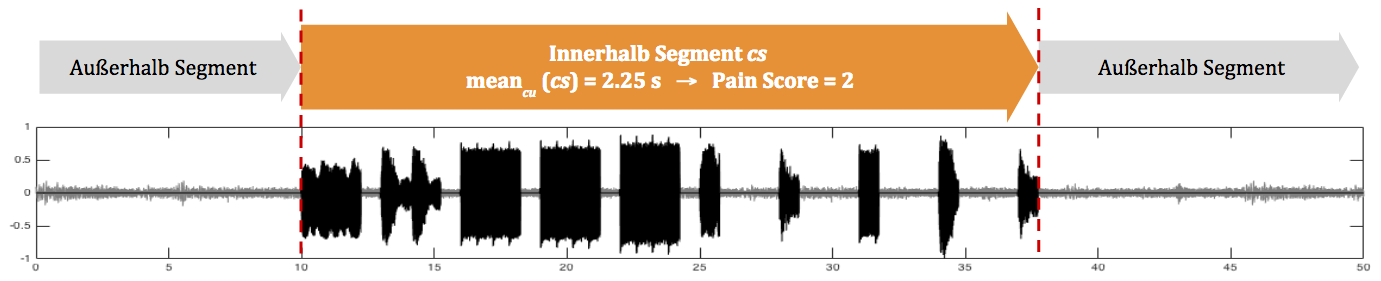
\includegraphics[width=1\textwidth]{bilder/regression_score_example04.png}
	\caption{Beispiel für die Ableitung von Pain Scores für ein Signal nach einer fiktiven Pain Scale ohne Beobachtungszeitraum oder Aktualisierungsintervall}
	\label{img:regression_score_example02}
\end{figure}


Abbildung \ref{img:regression_score_example01} zeigt ein Beispielsignal, für das Pain Scores nach dieser Pain Scale abgeleitet werden. In dem Signal werden die stimmhaften Signalbereiche schwarz und das Hintergrundrauschen grau dargestellt. Es sind insgesamt 10 Cry-Units zu erkennen. Die ersten fünf Cry-Units haben jeweils eine Länge von \SI{2.25}{\second}, die letzten fünf Cry-Units eine jeweilige Länge von \SI{0.75}{\second}. Das Signal wurde nach der in Kapitel \ref{sec:segmenting} beschriebenen Methode segmentiert mit $t_s = \SI{5}{\second}$ und so alle 10 Cry-Units zu einem Segment zusammengefasst. Das Segment erstreckt sich von Sekunde $10$ bis Sekunde $37.5$. Für das Segment wurde eine durchschnittliche Länge der Cry-Units von $mean_{cu}(cs) = \SI{1.5}{\second}$ gemessen und dem zufolge eine Pain Score von 2 abgeleitet. In diesem Fall wurde ohne Beobachtungs- und Aktualisierungsintervall gearbeitet. Wäre die Analyse also kontinuierlich vorgenommen worden, so wäre nach Feststellung der ersten Cry-Unit das Segment eröffnet, nach Überschreitung der maximal zulässigen Stille von $t_s = \SI{5}{\second}$ nach der 10. Cry-Unit das Segment geschlossen, und daraufhin $PS_{Fiction}(cs) = 2$ berechnet worden.

\begin{figure}[h]
	\centering
	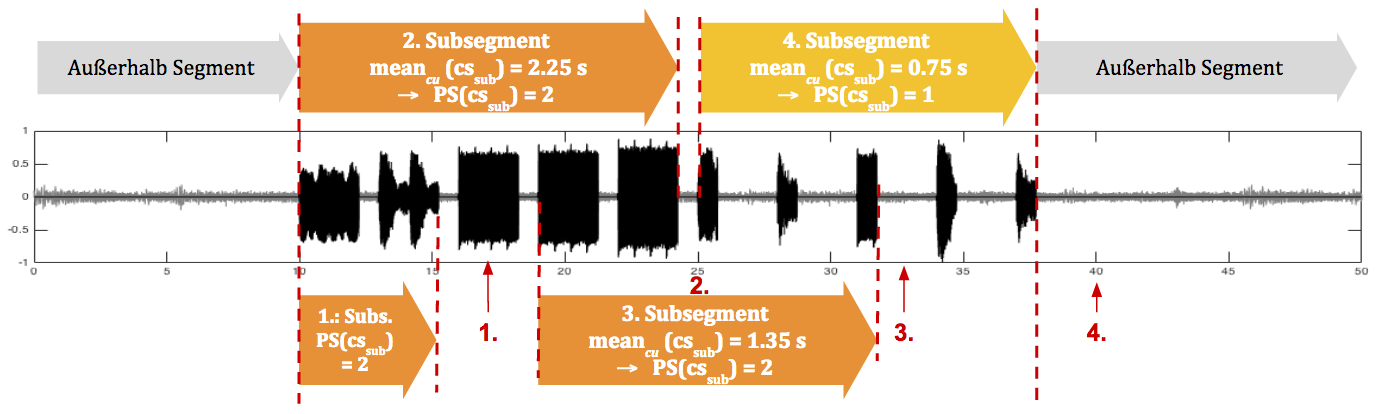
\includegraphics[width=1\textwidth]{bilder/regression_score_example05.png}
	\caption{Beispiel für die Ableitung von Pain Scores für ein Signal nach einer fiktiven Pain Scale mit $t_{act} = \SI{7.5}{\second}$ und $t_{obs} = \SI{15}{\second}$}
	\label{img:regression_score_example02}
\end{figure}

Abbildung \ref{img:regression_score_example03} zeigt die Ableitung der Schmerz Scores, wenn zusätzlich ein Aktualisierungsintervall von \SI{7.5}{\second} und ein Beobachtungszeitraum von \SI{15}{\second} gewählt wird. Nach dem das Segment durch die Cry-Unit an Sekunde 10 eröffnet wurde, werden Aktualisierungen zu den Zeitpunkten $t = \SI{17.5}{\second}, \SI{25}{\second}, \SI{32.5}{\second}$ und \SI{40}{\second} durchgeführt, verdeutlicht durch die kleinen, roten Pfeile in der Abbildung. Wie zu sehen ist, wird bei jeder Aktualisierung innerhalb des Beobachtungszeitraumes ein Subsegment gebildet, für das Subsegment die Features errechnet und die Pain Score abgeleitet. Der Anfangszeitpunkt jedes Subsegmentes ist der Anfang der erste Cry-Unit innerhalb des jeweiligen Beobachtungszeitraums, und das Ende des Subsegmentes das Ende letzten Cry-Unit im jeweiligen Beobachtungszeitraum. Beispielsweise erstreckt sich das bei der 3. Aktualisierung der Beobachtungszeitraum von $17.5 - \SI{32.5}{\second}$, das Subsegment jedoch von $19 - \SI{32}{\second}$ aufgrund der Lage der Cry-Units. Durch die Verwendung des Beobachtungs- und Aktualisierungsintervalls wird erkennbar, dass in diesem Beispiel der Schmerzgrad innerhalb des Segmentes nach hinten hin abnimmt.



\chapter{Visualisierung}
\label{sec:visualisation}

Ziel dieses Kapitels ist es, das erarbeitete Konzept zur Visualisierung der Pain Scores vorzustellen. Das Konzept wird anhand eines Beispielsignals erläutert, welches Aufnahmen des Weinenes eines Babys enthält. Das Signal wird in Abbildung \ref{img:visualisation_example_01} oben gezeigt. Der Signalausschnitt ist insgesamt 220 Sekunden lang. Die Abschnitte, die Stimme des Babys enthalten, werden Schwarz dargestellt, das Hintergrundrauschen grau. Das Signal wurde segmentiert mit $t_{s} = \SI{10}{\second}$ und so zwei Segmente gefunden. Die beiden Segmente sind $30.5$ Sekunden voneinander entfernt. 

Die Schmerzdiagnostik wird auf Basis zweier fiktiver Pain Scales durchgeführt, welche in Tabelle \ref{tab:fictional_painscales_viz} definiert werden. Die \glqq Length-Scale\grqq{} bewertet den Schmerzgrad nach der Länge des Weinens und vergibt einen maximalen Score on 2, die \glqq Min-Scale\grqq{} bewertet die Qualität des Weinens und vergibt einen maximalen Score von 3.

\begin{table}[h]
\centering
\caption{Fiktive Pain Scales zur Erläuterung der Visualisierung}
\label{tab:fictional_painscales_viz}
\begin{tabular}{@{}lll@{}}
\toprule
         & \glqq Length-Scale\grqq  & \glqq Min-Scale\grqq        \\ \midrule
0 Punkte & kein Weinen   & Lachen           \\
1 Punkt  & kurzes Weinen & leichtes Weinen  \\
2 Punkte & langes Weinen & mittleres Weinen \\
3 Punkte & -             & starkes weinen   \\ \bottomrule
\end{tabular}
\end{table}

Mit Hilfe einer der in Kapitel \ref{sec:deduction} vorgestellten Strategien wurden Vorschriften zur Ableitung des Schmerz Scores auf Basis der Segmentattribute definiert. Gleichung \ref{eq:ps_length} definiert die Funktion $PS_{Length}$, welche den Pain Score für Segmente nach der \glqq Length-Scale\grqq{} ableitet. Aus der Gleichung geht hervor, dass ein Score von 0 für ein Segment nicht abgeleitet werden kann, da die Anwesenheit eines Segmentes der Abwesenheit von Weinen implizit widerspricht. Gleichung \ref{eq:ps_length} definiert die Funktion $PS_{Max}$ zur Schmerzableitung nach der \glqq Min-Scale\grqq. 

\begin{equation}
PS_{Length}(cs) = \begin{cases}
 1 \quad ,  \text{wenn } \text{S-Length}(cs) \leq \SI{1}{\minute} \\
 2 \quad ,  \text{wenn } \text{S-Length}(cs) > \SI{1}{\minute}
 \end{cases}	
 \label{eq:ps_length}
\end{equation}

\begin{equation}
PS_{Min}(cs) = \begin{cases}
 0 \quad ,  \text{wenn } min_{cu}(cs) < \SI{0.3}{\second}\\
 1 \quad ,  \text{wenn } \SI{0.3}{\second} \leq min_{cu}(cs) \leq \SI{1}{\second}\\
 2 \quad ,  \text{wenn } \SI{1}{\second} < min_{cu}(cs) \leq \SI{2}{\second} \\
 3 \quad  \text{sonst }
 \end{cases}	
 \label{eq:ps_length}
\end{equation}

Mit Hilfe dieser Funktionen werden die Pain Scores für die beiden Segmente des Beispielsignals in Abbildung \ref{img:visualisation_example_01} abgeleitet. Es wurden dabei keine Aktualisierungsintervalle oder Beobachtungszeiträume genutzt. Das erste Segment nach der \emph{Length-Scale} einen Score von 1 und nach der \emph{Min-Scale} einen Score von 2. Das zweite Segment hat nach der \emph{Length-Scale} einen Score von 2 und nach der\emph{Min-Scale} einen Score von 1.

\begin{figure}[h]
	\centering
	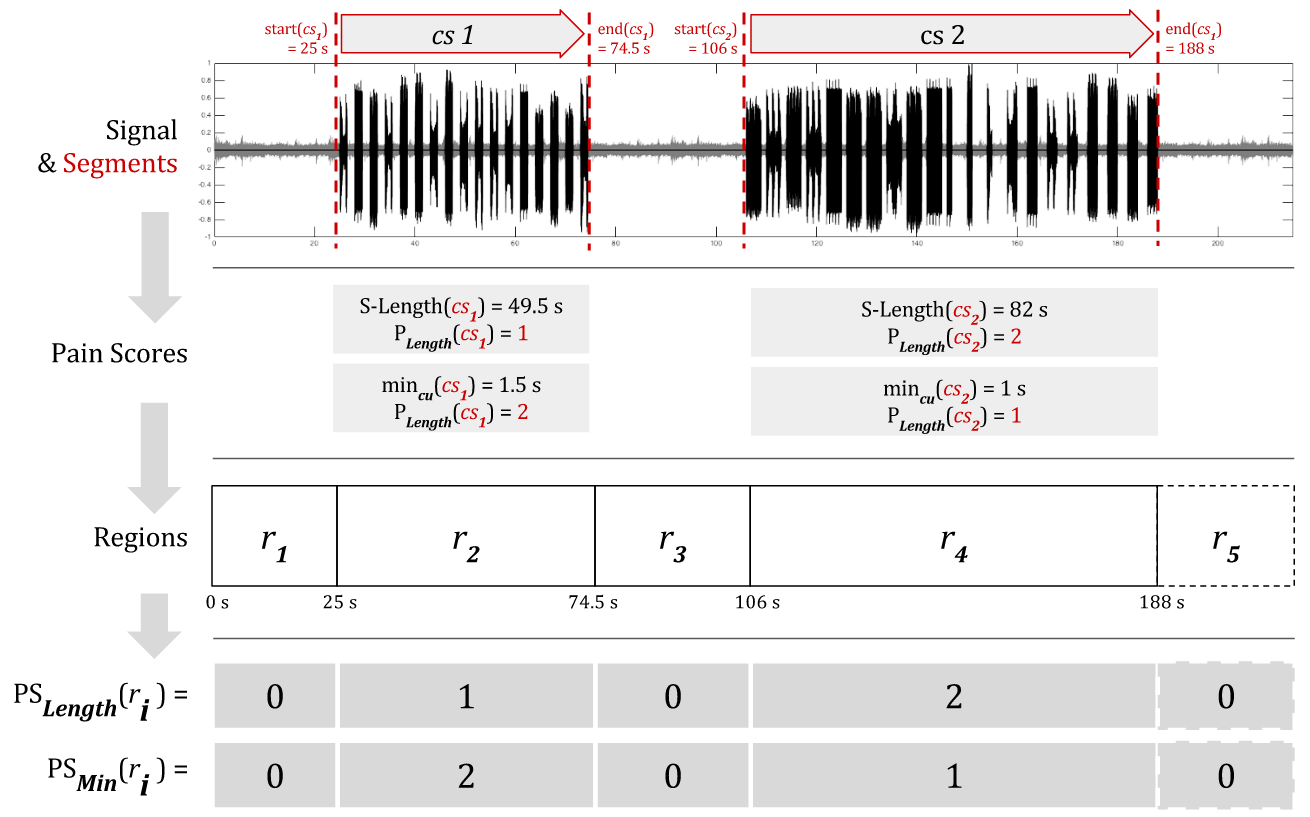
\includegraphics[width=1\textwidth]{bilder/visualisation_example_01.png}
	\caption{Oben: Ein Beispielsignal mit zwei Segmenten, die mit $t_s = \SI{10}{\second}$ gefunden wurden. Darunter: Pain Scores, die für die beiden Segmente berechnet wurden. Darunter: Schematische Darstellung des Signals als Regionen. Unten: Scores der Regionen.}
	\label{img:visualisation_example_01}
\end{figure}

Die grundlegende Idee der Visualisierung ist, den zeitlichen Verlauf des Signals schematisch als einen \emph{Balken} darzustellen. Dieser Balken wird in \emph{Regionen} eingeteilt. Eine Region $r$ beinhaltet entweder ein Cry-Segment oder den Stillebereich zwischen zwei Cry-Segmenten. Die Länge einer Region entspricht der zeitlichen Länge des jeweiligen Stille- oder Cry-Segments. In Abbildung \ref{img:visualisation_example_01} gibt es fünf Regionen $r_{1} , \ldots , r_5 $, wobei die Region $r_2$ und $r_4$ Cry-Segmente enthalten. Die letzte Region wurde noch nicht abgeschlossen, da angenommen wird, dass das Signal weiterhin kontinuierlich eingelesen wird.

Jeder Region wird ein Pain Score zugewiesen. Enthält die Region ein Segment, so wird der Score des Segmentes für die Region übernommen. Regionen ohne Segment bekommen, unabhängig von der verwendeten Pain Scale, einen Score von 0, wie Gleichung \ref{eq:region_score} definiert. Es wird somit angenommen, dass ein Score von 0 bei jeder Pain Scale den Zustand \glqq kein Schmerz\grqq{} codiert, was zumindest bei allen in Kapitel \ref{tab:painscores} vorgestellten Pain Scales der Fall ist. Abbildung \ref{img:visualisation_example_01} unten visualisiert diese Zuweisung von Scores zu den Regionen.

\begin{equation}
PS_{\text{Scale}}(r) = \begin{cases}
 0 \quad \quad \quad,  \text{wenn } r  \text{ kein Cry-Segment beinhaltet} \\
 PS_{\text{Scale}}(cs) \;, \text{wenn } r  \text{ ein Cry-Segment } cs \text{ beinhaltet}
 \end{cases}	
 \label{eq:region_score}
\end{equation}

Das Ziel ist es nun, jede Region mit einer Farbe einzufärben, die den entsprechenden Score anzeigt. Dazu wird für jede Pain Scale eine Funktion $F_{Scale}:S_{Scale} \mapsto P_{Scale}$ benötigt, welche einen Pain Score auf eine Farbe abbildet. Eine Abbildungsfunktion $F_{Scale}$ wird in diesem Zusammenhang als \emph{Farbschema} bezeichnet und der Funktionsbereich $P_{Scale}$ als \emph{Farbpalette}. Ein Farbschema soll die folgenden Kriterien erfüllen:

\begin{description}
\item[Injektivität] Jeder Score einer Scale soll anhand seiner Farbe eindeutig erkennbar sein. Dementsprechend soll gelten: $|S_{Scale}| \leq |P_{Scale}|$.
\item[Intuitive Farbsemantik durch Ampelschema] Ein Farbschema soll eine intuitive Zuordnung zwischen der Höhe des Score und der jeweiligen Farbe ermöglichen. In dieser Arbeit wurde sich für ein Ampelschema entschieden. Das heißt, dass für eine Pain Scale der jeweils niedrigste Score \glqq grün\grqq{}, der höchste Score \glqq rot\grqq{} und ein \glqq mittlerer\grqq{} Score als \glqq leicht rötliches gelb\grqq{} dargestellt wird. Definiert eine Pain Scale einen maximalen Score von 2, so wie beispielsweise das FLACC-System, so ergibt sich die Abbildung $F_{FLACC}(0) =  grün$, $F_{FLACC}(1) = gelb$, $F_{FLACC}(2) = rot$. Definiert die Pain Scale mehr Scores, wie beispielsweise das MBPS mit ingesamt fünf möglichen Scores, so müssen geeignete Zwischenfarben definiert werden. Daraus folgt, dass zwei Pain Scales, deren Menge an Scores gleich groß ist, das selbe Farbschema verwenden.
\item[Visuelle Gleichabständigkeit der Farben] Pain Scales definieren die Scores zwar in einer Reihenfolge, gewährleisten aber keine Vergleichbarkeit. Daher sollen die Farben eines Farbschemas eine \glqq visuelle Gleichabständigkeit\grqq{} gewährleisten. Damit ist gemeint, dass die Farben, auf die jeweils zwei aufeinander folgende Scores einer Scale abgebildet werden, visuelle den gleichen Abstand zueinander haben. So wird verhindert, dass ein Farbschema eine Nähe oder einen Abstand zwischen Scores suggeriert, der durch die jeweilige Pain Scale nicht codiert wird. 
\item[Visuelle Gleichwichtigkeit der Farben] Es kann nicht davon ausgegangen werden, dass ein bestimmter Score für die medizinische Fachkraft von größerem Interesse ist als ein anderer Score. Daher soll keine Farbe einer Farbpalette eine besondere Wichtigkeit suggerieren. Dies wird umgesetzt, in dem alle Farben einer Palette mit einer ähnliche Buntheit definiert werden.\cite{bigman}
\end{description}

Das Kriterium der Gleichabständigkeit legt die Verwendung des \emph{CIELAB}-Raum zur Farbdefinition für die Farbpaletten nahe. Der Farbraum ist in Bezug auf die menschliche Farbwahrnehmung \glqq gleichförmig\grqq. Das heißt, dass die euklidische Distanz zwischen zwei Farben im Farbraum ihrer wahrgenommenen Unterschiedlichkeit entsprechen. Da die Farbdefinition im CIELAB-Raum jedoch auf für den Menschen unintuitiven Parametern beruht, wird weiterhin der \emph{LCH}-Raum verwendet, der zylindrischen Transformation des CIELAB-Raumes. Dieser erlaubt die Farbdefinition auf Basis der für den Menschen intuitiveren Parameter \textbf{L}uminance (Luminanz), \textbf{C}hroma (Buntheit) und \textbf{H}ue (Farbton). Dies Erleichtert die Erfüllung der Farbsemantik, da sich die Farben Grün, Gelb und Rot in der H-Dimension des LCH-Raums in direkter Nachbarschaft befinden.\cite{palettes}\cite{johnstone}

Zur Zusammenstellung der konkreten Farbpaletten wird das Unterstützungwertkzeug \glqq Lch and Lab colour and gradient picker\grqq{} von David Johnstone verwendet.\footnote{Online unter: \url{http://davidjohnstone.net/pages/lch-lab-colour-gradient-picker}} Das Tool erlaubt die Wahl von $n$ Farben LCH-Raum, welche im folgenden als \glqq Fixpunkte\grqq bezeichnet werden. Diese werden ihrer Reihenfolge nach als Eckpunkte eines Pfades durch den Farbraum definiert. Auf Basis dieses Pfades generiert das Tool eine Farbpalette mit $m$ Farben. Ist $n = m$, so entspricht die Farbpalette den definierten Fixpunkten. Ist $m > n$, so findet das Tool die Zwischenfarben durch lineare Interpolation auf den Pfadkanten.

Ein \glqq reines Rot\grqq, codiert im RGB-Raum mit $[255,0,0]$, hat im LCH-Raum die Koordinaten $[53,105,40]$. \glqq Reines Grün\grqq{} hat die Koordinaten RGB $=[0,255,0]$, was LCH $= [88,120,136]$ entspricht. Das \glqq leicht rötliche Gelb\grqq wird definiert mit RGB $=[255,240,0] \hat{=}$LCH $= [93,93,99]$. Diese Farben haben im LCH Raum eine unterschiedliche Buntheit, weshalb sie in einer Farbpalette eine unterschiedliche Wichtigkeit suggerieren würden.\cite{bigman} Daher wurde die Buntheit aller drei Fixpunkte auf den niedrigsten der drei Werte, $93$, gesetzt. Die tatsächlichen Parameter der drei Fixpunkte \emph{Rot}, \emph{Gelb} und \emph{Grün} sind Tabelle \ref{tab:fixpoints} zu entnehmen. 

\begin{table}[h]
\centering
\caption{Fixpunkte als Basis der Farbpaletten}
\label{tab:fixpoints}
\begin{tabular}{@{}llll@{}}
\toprule
                                     & L      & C     & H      \\ \midrule
Rot   & 53     & 93    & 40     \\
Gelb  & 93     & 93    & 99     \\
Grün  & 88     & 93    & 136    \\ \bottomrule
\end{tabular}
\end{table}

Abbildung \ref{fig:color-swatches} zeigt die Farbpaletten, die mit Hilfe des Tools für zwei bis sieben Farben auf Basis dieser Fixpunkte erstellt wurden. Bei der Farbpalette mit ungerader Farbanzahl befinden sich die Fixpunkte an der ersten, letzten und mittleren Position, während die zusätzlichen Farben durch Interpolation erzeugt wurden. Bei den Farbpaletten mit gerader Farbanzahl wird der mittlere Fixpunkt, das Gelb, vom Tool entfernt.

\begin{figure}[h]
	\centering
	\includegraphics[width=0.75\textwidth]{bilder/colorpics.png}
	\caption{Erstellte Farbpaletten mit zwei bis sieben Farben inklusive der zugehörigen RGB-Koordinaten im Hex-Code.}
	\label{fig:color-swatches}
\end{figure}

Auf Basis die Farbpaletten wurden die Farbschemen $L_{n}: S_{Scale} \mapsto P_{Scale}$ definiert, abgebildet in Tabelle \ref{tab:color_shemes}. Es gilt $n = |S_{Scale}|$. Die Wahl des Farbschemas zur Visualisierung einer Pain Scale richtet sich also allein nach der jeweiligen Anzahl definierter Pain Scores, also $F_{Scale} = L_{|S_{Scale}|}$. Soll also beispielsweise die \glqq Length-Scale\grqq{} visualisiert werden, so wird das Farbschema $F_{\text{Length-Scale}} = L_3$ verwendet. Ein Pain Score von $s = 0$ wird durch das Grün mit den RGB-Kooridaten $\#6efa56$ codiert, 1 durch \#6efa56 und 2 durch \#6efa56.

Es wurden keine Farbschemen für $n<1$ definiert, da eine Pain Scale mit nur einer Score nicht sinnvoll ist, sowie keine Farbpaletten mit $n>7$, da keine der in Kapitel \ref{sec:painScores} gelisteten Pain Scales mehr als 7 Scores verwendet. Die Farbpaletten der Schemen $S_2, S_3, S_5$ und $S_7$ wurden direkt aus den Farbpaletten mit der jeweiligen Anzahl an Farben übernommen, die mit Hilfe des Tools von David Johnstone erzeugt wurden (Siehe Abbildung \ref{fig:color-swatches}). Die durch das Tool erzeugten Farbpalette mit vier und sechs Farben wurde nicht für die Schemen $S_3$ und $S_6$ übernommen, da in ihr der Gelbe Fixpunkt nicht enthalten war. Stattdessen wurden die jeweils nächst höheren Farbpaletten unter Auslassung des ersten Grüns verwendet. 

\begin{table}[h]
\centering
\caption{Definition der Farbschemen zur Visualisierung der Pain Scales. Die Farbwerte werden als Hexadezimal-Codes für den RGB-Farbraum angegeben. }
\label{tab:color_shemes}
\begin{tabular}{@{}clllllll@{}}
\toprule
              $s=$         & $0$                                                     & $1$                                                     & $2$                                                     & $3$                                                     & $4$                                                     & $5$                                                     & $6$                                                     \\ \midrule
\multicolumn{1}{l|}{$L_2(s) = $} & \multicolumn{1}{l|}{\cellcolor[HTML]{6EFA56}\#6efa56} & \multicolumn{1}{l|}{\cellcolor[HTML]{F32D16}\#f32d16} &                                                       &                                                       &                                                       &                                                       &                                                       \\ \cmidrule(lr){2-4}
\multicolumn{1}{l|}{$L_3(s) = $} & \multicolumn{1}{l|}{\cellcolor[HTML]{6EFA56}\#6efa56} & \multicolumn{1}{l|}{\cellcolor[HTML]{FFF000}\#fff000} & \multicolumn{1}{l|}{\cellcolor[HTML]{F32D16}\#f32d16} &                                                       &                                                       &                                                       &                                                       \\ \cmidrule(lr){2-5}
\multicolumn{1}{l|}{$L_4(s) = $} & \multicolumn{1}{l|}{\cellcolor[HTML]{B6F52B}\#bff729} & \multicolumn{1}{l|}{\cellcolor[HTML]{FFF000}\#fff000} & \multicolumn{1}{l|}{\cellcolor[HTML]{F98E0B}\#ff9900} & \multicolumn{1}{l|}{\cellcolor[HTML]{F32D16}\#f32d16} &       &                                                       &                                                       \\ \cmidrule(lr){2-6}
\multicolumn{1}{l|}{$L_5(s) = $} & \multicolumn{1}{l|}{\cellcolor[HTML]{6EFA56}\#6efa56} & \multicolumn{1}{l|}{\cellcolor[HTML]{BFF729}\#bff729} & \multicolumn{1}{l|}{\cellcolor[HTML]{FFF000}\#fff000} & \multicolumn{1}{l|}{\cellcolor[HTML]{F98E0B}\#ff9900} & \multicolumn{1}{l|}{\cellcolor[HTML]{F32D16}\#f32d16} &                                                       &                                                       \\ \cmidrule(lr){2-7}
\multicolumn{1}{l|}{$L_6(s) = $} & \multicolumn{1}{l|}{\cellcolor[HTML]{A7F938}\#a7f938} & \multicolumn{1}{l|}{\cellcolor[HTML]{D5F519}\#d5f519} & \multicolumn{1}{l|}{\cellcolor[HTML]{FFF000}\#fff000} & \multicolumn{1}{l|}{\cellcolor[HTML]{FFB700}\#ffb700} & \multicolumn{1}{l|}{\cellcolor[HTML]{FF7A00}\#ff7a00} & \multicolumn{1}{l|}{\cellcolor[HTML]{F32D16}\#f32d16} &                                                       \\ \cmidrule(l){2-8} 
\multicolumn{1}{l|}{$L_7(s) = $} & \multicolumn{1}{l|}{\cellcolor[HTML]{6EFA56}\#6efa56} & \multicolumn{1}{l|}{\cellcolor[HTML]{A7F938}\#a7f938} & \multicolumn{1}{l|}{\cellcolor[HTML]{D5F519}\#d5f519} & \multicolumn{1}{l|}{\cellcolor[HTML]{FFF000}\#fff000} & \multicolumn{1}{l|}{\cellcolor[HTML]{FFB700}\#ffb700} & \multicolumn{1}{l|}{\cellcolor[HTML]{FF7A00}\#ff7a00} & \multicolumn{1}{l|}{\cellcolor[HTML]{F32D16}\#f32d16} \\ \bottomrule
\end{tabular}
\end{table}

Abbildung \ref{fig:viz_without_t_01} zeigt die Visualisierung der Schmerzdiagnostik für das Beispielsignal mit der \glqq Length-Scale\grqq{} und der \glqq Min-Scale\grqq{}, die durch das Einfärben der in Abbildung \ref{img:visualisation_example_01} erläuterten Regionen entsteht. Wie bereits erläutert, verwendet die \glqq Length-Scale\grqq{} das Farbschema $L_3$. Die \glqq Min-Scale\grqq{} definiert insgesamt 4 Scores und verwendet somit das Farbschema $L_4$.

\begin{figure}[h]
	\centering
	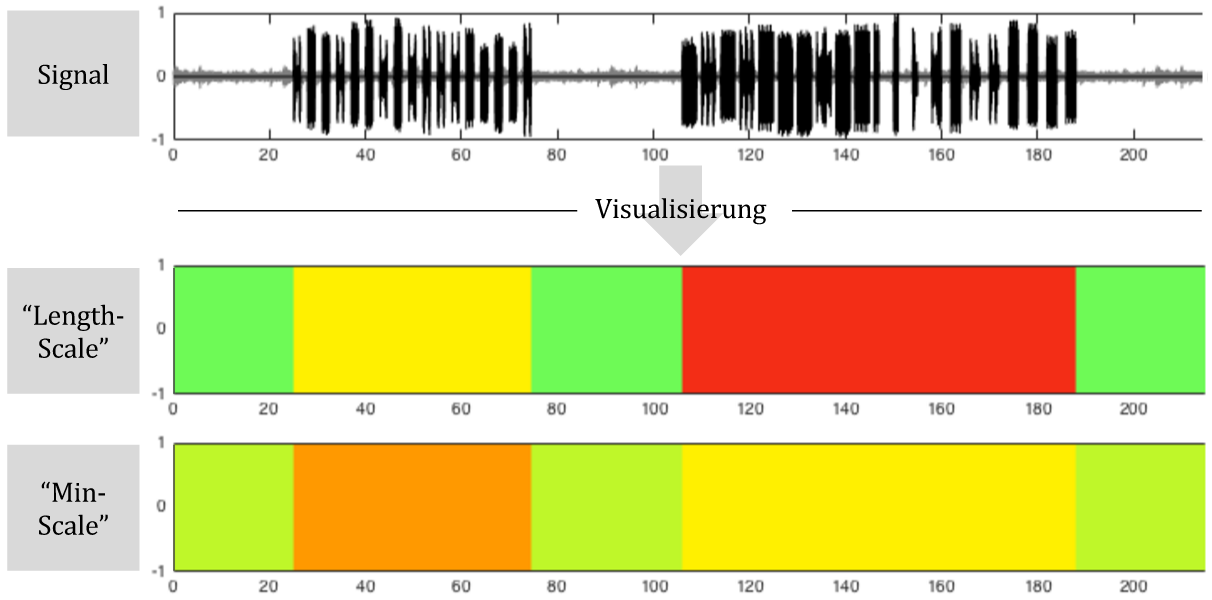
\includegraphics[width=1\textwidth]{bilder/viz_without_t_02.png}
	\caption{Visualisierung der \glqq Length-Scale\grqq{} und der \glqq Min-Scale\grqq{} für das Beispielsignal. }
	\label{fig:viz_without_t_01}
\end{figure}

Da in diesem Beispiel kein Aktualisierungsintervall eingesetzt wurde, gibt es keine überlappenden Regionen. Abbildung \ref{fig:viz_multiple_regions} veranschaulicht, wie durch die Verwendung eines Aktualisierungsintervalls überlappende Regionen entstehen. Oben in der Abbildung ist das Beispielsignal zu sehen, welches mit $t_s = \SI{10}{\second}$ segmentiert wurde. Es wurde ein Aktualisierungsintervall von  $t_{act} = \SI{20}{\second}$ und $t_{obs} = \infty$ verwendet. Die Aktualisierungszeitpunkte sind durch kleine Pfeilge angegeben. Unten sind die aus den Subsegmenten entstandenen, einander überlappenden Regionen abgebildet. Für jede Region wir der Score angegeben, der sich nach der Diagnostik der Min-Scale ergibt, sowie jede Region nach dem Schema $L_4$ eingefärbt.

\begin{figure}[h]
	\centering
	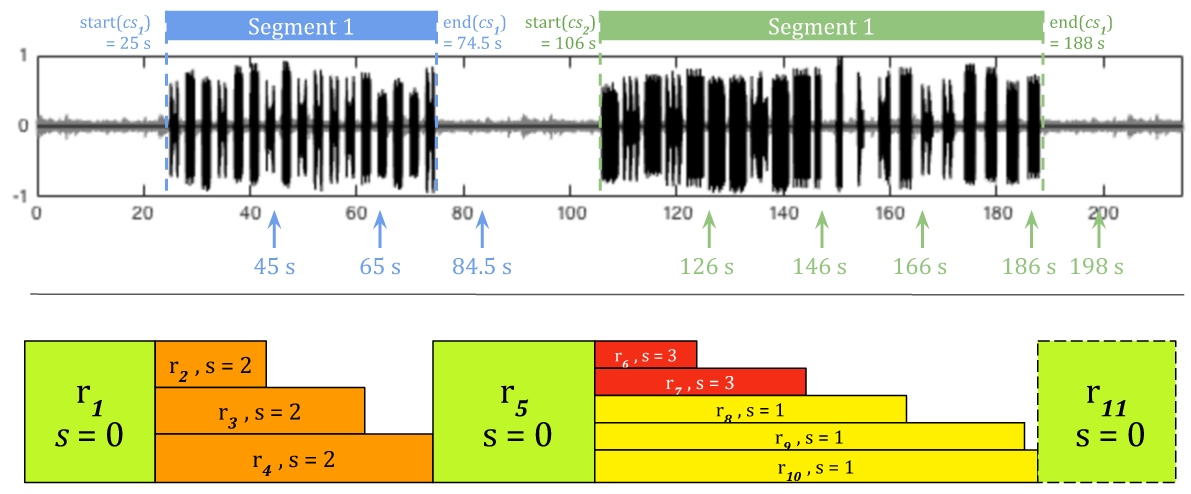
\includegraphics[width=1\textwidth]{bilder/viz-multiple-regions.png}
	\caption{Oben: Beispielsignal mit zwei Segmenten. Unten: Überlappende Regionen, eingefärbt nach dem Farbschema der Min-Scale.}
	\label{fig:viz_multiple_regions}
\end{figure}

Die Darstellung aus Abbildung \ref{fig:viz_multiple_regions} dient nur der Veranschaulichung des Prinzips der überlappenden Regionen, eignet sich aber nicht für eine tatsächliche Visualisierung. Es werden zwei Möglichkeiten zur Visualisierung einander überlappender Regionen vorgeschlagen:
\begin{itemize}
\item Die Region mit dem späteren Endzeitpunkt wird \glqq auf\grqq{} die Regionen mit einem früheren Endzeitpunkt gelegt. So wird der aktuell diagnostizierte Score wird in den Vordergrund gestellt, der zeitliche Verlauf der abgeleiteten Schmerz Scores geht jedoch verloren. Abbildung \ref{fig:viz_act_over} zeigt dieses Prinzip an einem Beispiel. In diesem Fall wurde das Beispielsignal erst bis zu Sekunde $146$ eingelesen, das zweite Segment ist noch geöffnet. Bei der Aktualisierung zum Zeitpunkt $t=\SI{146}{\second}$ wird nach der Min-Scale ein Score von 3 abgeleitet und die Region dementsprechend rot eingefärbt. Das Signal wird nun weiter eingelesen. Bei der nächsten Aktualisierung bei $t=\SI{166}{\second}$ wird ein Score von 1 abgeleitet und die so gelb gefärbte Region \glqq auf\grqq die rot gefärbte Region gelegt.

\begin{figure}[h]
	\centering
	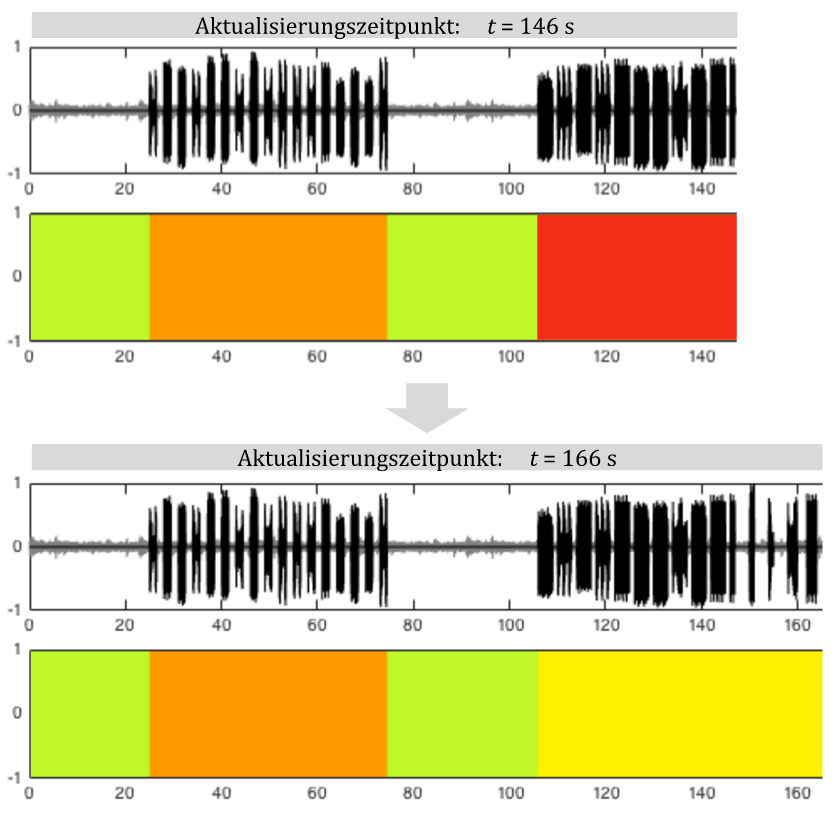
\includegraphics[width=0.7\textwidth]{bilder/viz_act_over.png}
	\caption{Visualisierung der Schmerzdiangostik mit der Min-Scale bei Aktualisierungen. Die aktuellere Region wird \emph{über} ältere Regionen gelegt.}
	\label{fig:viz_act_over}
\end{figure}

\item Die Region mit dem späteren Endzeitpunkt wird \glqq unter\grqq{} die Regionen mit einem früheren Endzeitpunkt gelegt. So wird der zeitliche Verlauf des diagnostizierten Schmerzes in den Vordergrund gestellt. Abbildung \ref{fig:viz_act_under} zeigt die Visualisierung der Schmerzdiagonstik mit der Min-Scale nach diesem Prinzip. Wie zu sehen ist, bleibt auch nach Aktualisierung der Schmerzscore des zweiten Segmentes auf 1 erkennbar, dass bei der früheren Aktualisierung ein Score von 3 abgeleitet wurde.

\begin{figure}[h]
	\centering
	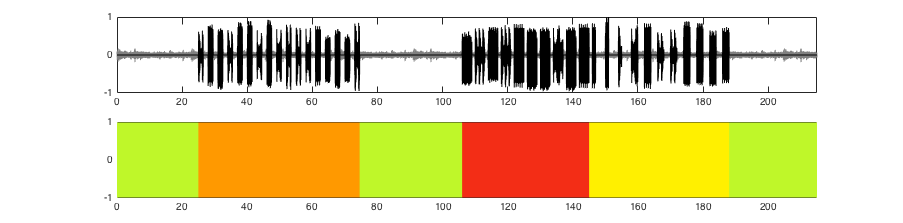
\includegraphics[width=1\textwidth]{bilder/viz_act_under.png}
	\caption{Visualisierung der Schmerzdiangostik mit der Min-Scale bei Aktualisierungen. Die aktuellere Region wird \emph{unter} ältere Regionen gelegt.}
	\label{fig:viz_act_under}
\end{figure}
 
\end{itemize}


\chapter{Zusammenfassung}

\bibliographystyle{plain}
\bibliography{references}


\begin{appendices}
\begin{landscape}
\begin{table}[h]
\centering
\caption{Accuracy-Werte der Grenzwertfindung mit REPTree}
\label{tab:reptree_results}
\begin{tabular}{@{}lllllllllllll@{}}
\toprule
$SNR_{Training}$ & \SI{3}{\decibel}     &         &         &                  & \SI{50}{\decibel}    &         &         &                  & 50+\SI{3}{\decibel} &        &         &                  \\ 
$SNR_{Test}$     & \SI{3}{\decibel}     & \SI{50}{\decibel}    & \SI{7}{\decibel}*    & Mean             & \SI{3}{\decibel}     & \SI{50}{\decibel}    & \SI{7}{\decibel}*    & Mean             & \SI{3}{\decibel}     & \SI{50}{\decibel}    & \SI{7}{\decibel}*    & Mean             \\ \midrule
Zeit           & 77.81\% & 79.02\% & 86.04\% & 80,96\%          & 49.33\% & 94.70\% & 48.66\% & 64,23\%          & 77.54\% & 92.47\% & 84.38\% & 84,80\%          \\
Freq           & 82.05\% & 89.28\% & 82.71\% & 84,68\%          & 70.52\% & 94.37\% & 55.06\% & 73,31\%          & 81.75\% & 91.22\% & 74.90\% & 82,62\%          \\
Ceps           & 88.98\% & 94.72\% & 92.96\% & \textbf{92,22\%} & 86.83\% & 94.68\% & 92.83\% & \textbf{91,45\%} & 88.98\% & 94.72\% & 92.96\% & \textbf{92,22\%} \\
Corr           & 80.45\% & 73.47\% & 84.89\% & 79,60\%          & 73.07\% & 87.14\% & 77.98\% & 79,39\%          & 77.90\% & 84.88\% & 82.84\% & 81,87\%          \\
Zeit+Freq      & 82.05\% & 89.28\% & 82.71\% & 84,68\%          & 70.52\% & 94.37\% & 55.06\% & 73,31\%          & 81.75\% & 91.22\% & 74.90\% & 82,62\%          \\
Zeit+Ceps      & 88.98\% & 94.72\% & 92.96\% & \textbf{92,22\%} & 86.83\% & 94.68\% & 92.83\% & \textbf{91,45\%} & 88.98\% & 94.72\% & 92.96\% & \textbf{92,22\%} \\
Zeit+Corr      & 80.45\% & 73.47\% & 84.89\% & 79,60\%          & 49.33\% & 94.70\% & 48.66\% & 64,23\%          & 80.32\% & 92.35\% & 88.22\% & 86,96\%          \\
Freq+Ceps      & 88.98\% & 94.72\% & 92.96\% & \textbf{92,22\%} & 70.65\% & 94.75\% & 55.06\% & 73,49\%          & 88.98\% & 94.72\% & 92.96\% & \textbf{92,22\%} \\
Freq+Corr      & 82.05\% & 89.28\% & 82.71\% & 84,68\%          & 70.52\% & 95.60\% & 95.60\% & 87,24\%          & 81.75\% & 94.42\% & 74.90\% & 83,69\%          \\ \bottomrule
\end{tabular}
\end{table}

 \begin{figure}[h]
	\centering
	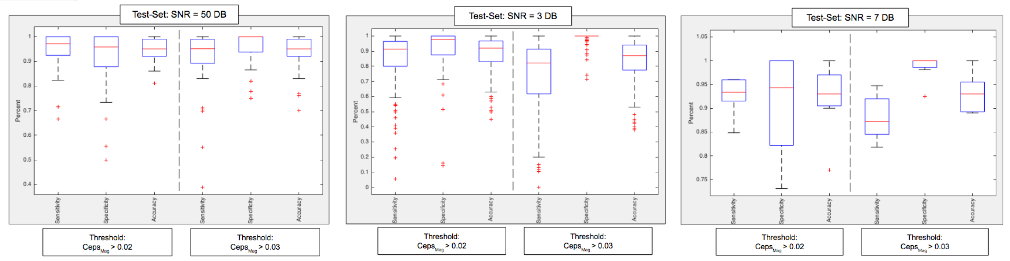
\includegraphics[width=1.2\textwidth]{bilder/all_boxplots.png}
	\caption{Boxplot-Auswertung über Sensitivity, Specificity und Accuracy der beiden VAD-Modelle}
	\label{img:boxplots}
\end{figure}

\end{landscape}

\end{appendices}



\end{document}
